\documentclass[a4paper,12pt]{scrartcl}
\usepackage[utf8]{inputenc}
\usepackage[ngerman]{babel}
\usepackage{graphicx} %Grafiken einbinden   [draft]
\usepackage{wrapfig} %Grafiken von Text umfliessen lassen
\usepackage{multicol} %zweispaltiger Text
\usepackage{multirow} %mehrere Tabellenzeilen zu einer zusammenfassen
% \usepackage{tabularx} %automatische Zeilenumbrüche in Tabellenzellen
% \usepackage{array} %für Tabularx benötigt
\usepackage{colortbl} %farbige Tabellen
\usepackage{color} %farbige Diagramme
\usepackage{textcomp} %Lexikon-Zeichen
\usepackage{rotating} %Rotation von Schrift
\usepackage{eurosym} %EURO-Symbol
\usepackage{wallpaper} %Bilder auch ans Hintergrundbilder einbinden
\usepackage[a4paper,left=15mm,right=15mm, top=12mm, bottom=26mm]{geometry} %Seitenränder
%\geometry{a4paper,left=40mm,right=40mm, top=20mm, bottom=28mm}
\usepackage{hyperref} %Um in der PDF-Version klickbare Hyperlinks zu haben
\usepackage{color} % für Farben im allgemeinen
\usepackage{colortbl} % für die Hintergrundfarbe einzelner Zellen in Tabellen
\usepackage{booktabs}
\usepackage{soul} % Zum durchstreichen
\usepackage[final]{pdfpages} % support for pdf inclusion

\usepackage{paralist}

%VERÄNDERBARE KOMMANDOS

\newcounter{mycounter}  
\newenvironment{noindEnumerate}
 {\begin{list}{\arabic{mycounter}.~~}{\usecounter{mycounter} \labelsep=0pt \labelwidth=0pt \leftmargin=0pt \itemindent=0pt \itemsep=-5pt}}
 {\end{list}}
\newenvironment{noindItemize}
 {\begin{list}{\labelitemi}{\usecounter{mycounter} \labelsep=5pt \labelwidth=0pt \leftmargin=5pt \itemindent=0pt \itemsep=-5pt}}
 {\end{list}}

\newenvironment{fancyblock}[1]
{	\vspace{3mm}
	\hspace{5mm}
	\begin{tabular}{p{15cm}}
	\textbf{#1}\\
	\midrule
}
{\end{tabular}\vspace{3mm}}

%Datei-Endung eps für latex > dvips > ps2pdf
%Datei-Endung png oder jpg für pdflatex, Programm sucht sich das richtige Format automatisch aus
\newcommand{\emailfachschaft}{\raisebox{-0.5mm}{
\includegraphics{bitmaps/email_fachschaft}}~}
\newcommand{\emailstugug}{\raisebox{-0.5mm}{\scalebox{0.23}{
\includegraphics{bitmaps/email_stugug}}}}
\newcommand{\emailwohnen}{\raisebox{-0.5mm}{\scalebox{0.23}{
\includegraphics{bitmaps/email_wohnen}}}}
\newcommand{\emailinfo}{\raisebox{-0.5mm}{\scalebox{0.23}{
\includegraphics{bitmaps/email_info}}}}

\newcommand{\spaltenanfang}{\begin{multicols}{2}}
\newcommand{\spaltenende}{\end{multicols}}
%\newcommand{\spaltenanfang}{ }
%\newcommand{\spaltenende}{ }

\setlength{\columnsep}{8mm}

% Remove indentation + add vertical space between paragraphs
\usepackage{parskip}

\newcommand{\profSchnBild}{
   \begin{wrapfigure}{l}{3cm}
   \begin{center}
   \includegraphics[scale=0.5]{comics/single/prof_schn}
   \end{center}
   \end{wrapfigure}
 }
 

\begin{document}

\begin{titlepage}

\thispagestyle{empty}
\title{\Huge{Don't Panic! 42}}
\author{Magazin für die OE WS 2015}
\date{Herausgegeben von der Fachschaft Informatik}


%\begin{document}

\ThisCenterWallPaper{1.0}{bilder/bender_titelseite4}
\maketitle
\newpage
\end{titlepage}


{
\small
\tableofcontents
}

\newpage
%%%%%%%%%%%%%%%%%%%%%%%%%%%%%%%%%%%%%%%%%%%%%%%%%%%%
\spaltenanfang
\noindent\textbf{Studentische Vertretung der Lehreinheit Informatik der Johann Wolfgang Goethe-Universität Frankfurt am Main}\\
Robert-Mayer-Straße 11 - 15\\
D-60325 Frankfurt am Main\\
\url{www.fsinf-frankfurt.de}\\
\url{www.fsinf-forum.de}\\
\emailfachschaft\\
%~\newline
Don‘t Panic! 42\\
OE SoSe 2016\\
Oft überarbeitete und erweiterte Auflage\\
Version der Ausgabe: 2.0\\
April 2016\\
Erscheinungsweise: jedes Semester\\
Auflage: 250\\
Druck und Bindung: HRZ Druckzentrum

\spaltenende

\newpage


%%%%%%%%%%%%%%%%%%%%%%%%%%%%%%%%%%%%%%%%%%%%%%%%%%%%
\section{Hallo erstmal …}

\spaltenanfang
\spaltenanfang
Herzlich willkommen bei uns am Fachbereich! Was du gerade in deinen Händen
hältst, ist die Zeitschrift der diessemestrigen Orientierungsveranstaltung, die
wir „Don’t Panic“ getauft haben. \textbf{Don’t Panic!} - das soll auch als
Motto über der ganzen Veranstaltung stehen. Diesmal nur leicht editiert,
da wir nachdem wir das letzte mal alles in einer Nacht geschrieben haben,
so viele Kommafehler eingebaut hatten, das die \textbf{Don't Panic!} eine Seite
l"anger wurde. 


Naja,jetzt ist erst mal wieder Semesteranfang, und es haben sich lauter Menschen entschlossen,
in Frankfurt einen Studiengang der Informatik aufzunehmen. Darunter sind
Einige, die schon vorher etwas anderes studiert haben oder von einer anderen
Hochschule kommen. Die kennen sich meist schon recht gut im Uni-Dschungel aus,
und auch die ganzen Begriffe, Abkürzungen und Redewendungen sind für sie keine
böhmischen Dörfer mehr. Aber für einen beachtlichen Teil der Erstsemester ist
erfahrungsgemäß so ziemlich alles neu. Und deswegen werden wir uns bemühen,
euch während dieser Orientierungsveranstaltung so ziemlich alles zu erklären.
Ihr werdet hoffentlich schnell merken, dass das alles halb so wild ist und kein
Grund zur Panik besteht, also \textbf{Don’t Panic!} Bei dieser
Orientierungsveranstaltung haben wir uns im Wesentlichen zwei Ziele gesetzt:


Wir wollen euch mit allen notwendigen Informationen versorgen, damit ihr an
eurem ersten Tag in der Uni wenigstens so ungefähr wisst, wo die wichtigsten
Einrichtungen sind, welche Veranstaltungen so laufen und welche davon für euch
Sinn machen. Wir wollen euch ein paar Ratschläge und Tipps mit auf den Weg
geben, und nicht zuletzt können wir euch von einer großen Sammlung von Fehlern
berichten, die wir gemacht haben und die \textsl{ihr} ja nicht unbedingt noch
mal machen müsst.


Das Uni-Leben und das Informatik-Studium bringen viele Begriffe mit sich, die
euch vielleicht unbekannt sind. Vielleicht möchtet ihr einige Stichworte auch
noch einmal in kompakter Form nachlesen. Aus diesem Grund haben wir euch ein
Glossar der wichtigsten Begriffe zusammengestellt.


Aber wir möchten auch, dass ihr euch heute gegenseitig ein
bisschen kennenlernt, damit euch am nächsten Montag wenigstens schon ein paar
Gesichter bekannt vorkommen, wenn der Stress losgeht. Ganz generell empfehlen
wir, sich in kleinen Gruppen zusammenzutun. In einer Gruppe weiß eigentlich
immer jemand, was wo aushängt, bis wann man sich irgendwo eingetragen haben
muss und Vieles mehr. Auch das eigentliche Studieren, das Lernen und das Lösen
von Aufgaben ist in einer Gruppe wesentlich erfolgversprechender und mit
Sicherheit angenehmer.\\
\spaltenende

\spaltenende

\vspace{10mm}
\begin{center}
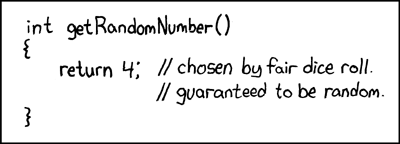
\includegraphics[scale=1.0]{comics/random_number}
\end{center}

%\includepdf[pages=1]{tabellen/zeitplan.pdf}
%% \newcommand{\verbreiterung}{\parbox{48mm}{~}}

% \begin{addmargin}[-2mm]{0cm}

% \begin{center}
% \begin{tabular}{|c|c|c|c|}
% \hline Zeit & Mittwoch & Donnerstag & Freitag \\ 
% \hline 8:00 & Frühstück & \multirow{2}{*}{Frühstück} & \multirow{2}{*}{Frühstück}  \\ 
            % & Begrüßung &  &  \\ 
% \cline{1-1}\cline{3-4} 9:00 & Gruppenaufteilung & \multirow{2}{*}{Erklärung zu Formalitäten} & Ergebnisse der Klausur \\ 
% \cline{2-2}                 & Vorstellung:      &                                            & Preisverleihung \\
% \cline{1-1}\cline{3-4} 10:00 & Bachelor  & \multirow{2}{*}{Klausur} &  \\ 
                  % & Anwendungsfach &  &  \\ 
% \cline{1-1}\cline{3-3} 11:00 & Lehramt, Master & \multirow{4}{*}{Vorträge der Profs} &  \\ 
% \cline{2-2}       & \multirow{3}{*}{Essen} &  & Vorstellung Gewerkschaft \\ 
% \cline{1-1} 12:00 &                        &  & /Unternehmensbesuch? \\ 
                  % &                        &  &  \\ 
% \cline{1-3} 13:00 & \multirow{3}{*}{Gruppenarbeit} &  &  \\ 
       % &  &  &  \\ 
% \cline{1-1}\cline{4-4} 14:00 &  & Rundgang & \multirow{6}{*}{Kneipenabend} \\ 
% \cline{2-2}       & \multirow{5}{*}{Vorträge} & Grill \& Bier  &  \\ 
% \cline{1-1} 15:00 &  &  &  \\ 
                  % &  &  &                \\ 
% \cline{1-1} 16:00 &  &  &  \\ 
 % & \verbreiterung & \verbreiterung & \verbreiterung \\
% \hline
% \end{tabular} 
% \end{center}


% \end{addmargin}
\section{Zeitplan der OE}
\includegraphics[width=\linewidth]{bitmaps/OE2011SS_Zeitplan_Bender}


%%%%%%%%%%%%%%%%%%%%%%%%%%%%%%%%%%%%%%%%%%%%%%%%%%%%

\newpage
\section{Euer Stundenplan zum Ausfüllen}
\newcommand{\x}{\parbox[0pt][2.7cm][c]{3.7cm}{\hspace{3.7cm}} }
\newcommand{\xT}{\parbox[0pt][1.6cm][c]{1.9cm}{\hspace{3.7cm}} }
% --- Farbdefinitionen ----------------------------------------
\definecolor{hellgrau}{rgb}{0.95,0.95,0.95}

%\begin{sidewaystable}
%\begin{addmargin}[-2mm]{0cm}

%\begin{center}
%\begin{tabular}{|c|c|c|c|c|c|}
%\hline Zeit & Montag & Dienstag & Mittwoch & Donnerstag & Freitag \\
%\hline 8-10  & \x & \x & \x & \x & \x \\
%\hline 10-12 & \x & \x & \x & \x & \x \\
%\hline 12-14 & \x & \x & \x & \x & \x \\
%\hline 14-16 & \x & \x & \x & \x & \x \\
%\hline 16-18 & \x & \x & \x & \footnotesize 16:00 : Fachschaftstreffen & \x \\
%\hline ab 18 & \x & \x & \x & \x & \x \\
%\hline
%\end{tabular}
%\end{center}

%\end{addmargin}
%\end{sidewaystable}

\vspace{23.6cm} % ein Korrekturabstand wg. Drehen
\begin{center}
\begin{rotate}{90}
\begin{tabular}{|c|c|c|c|c|c|}
\hline \cellcolor{black} \xT
	& \cellcolor{black} \textcolor{white}{\textbf{Montag}}
	& \cellcolor{black} \textcolor{white}{\textbf{Dienstag}}
	& \cellcolor{black} \textcolor{white}{\textbf{Mittwoch}}
	& \cellcolor{black} \textcolor{white}{\textbf{Donnerstag}}
	& \cellcolor{black} \textcolor{white}{\textbf{Freitag}} \\
\hline 8:00-10:00  & \x & \x & \x & \x & \x \\
\hline  \cellcolor{hellgrau}10:00-12:00 &  \cellcolor{hellgrau} \x &  \cellcolor{hellgrau} \x &  \cellcolor{hellgrau} \x &  \cellcolor{hellgrau} \x &  \cellcolor{hellgrau} \x \\
\hline 12:00-14:00 & \x & \x & \x & \x & \x \\
\hline  \cellcolor{hellgrau} 14:00-16:00 &  \cellcolor{hellgrau} \x &  \cellcolor{hellgrau} \x &  \cellcolor{hellgrau} \x &  \cellcolor{hellgrau} \x &  \cellcolor{hellgrau} \x \\
\hline 16:00-18:00 & \x & \x & \x & \footnotesize & \x \\
\hline  \cellcolor{hellgrau} 18:00-20:00 &  \cellcolor{hellgrau} \x &  \cellcolor{hellgrau} \x &  \cellcolor{hellgrau} \x &  \cellcolor{hellgrau} \x &  \cellcolor{hellgrau} \x \\
\hline
\end{tabular}
\end{rotate}
\end{center}



%%%%%%%%%%%%%%%%%%%%%%%%%%%%%%%%%%%%%%%%%%%%%%%%%%%%

\newpage
\section{So einfach ist das alles gar nicht \dots}
\spaltenanfang
Wenn man am ersten Montag in seine erste Vorlesung geht, ist es wohl für die
meisten ein ungewohntes Gefühl. Gerade von der Schule, aus einem freiwilligen
sozialen Jahr oder aus einer Ausbildung gekommen, kommt es einem sehr komisch
vor, in einem relativ großen Hörsaal zu sitzen und sich den Vortrag eines
Professors anzuhören. Vor allem macht man sich bei einigen Veranstaltungen sehr
schnell Gedanken, warum man sich so früh in die Uni begibt, wenn man sich den
Inhalt der Vorlesung auch im Internet herunterladen und selbst lesen könnte. 
Sicherlich mag ein gemütliches Bett sehr verlockend sein, aber die Erfahrung
zeigt, dass der Lerneffekt wesentlich höher ist, wenn man seinen inneren
Schweinehund überwindet und regelmäßig in die Veranstaltungen geht und auch
versucht, den Stoff richtig nachzubereiten.  Die Zwanglosigkeit, die das
universitäre Studium mit sich bringt, stellt wohl jeden von uns anfangs vor die
Aufgabe zu lernen, sich selbstverantwortlich durch sein Studium zu kämpfen. Man
wird vor viele Fragen gestellt. Welche Veranstaltungen soll ich besuchen, mache
ich lieber mehr davon, oder ist es vielleicht besser, am Anfang nicht das
Maximum an Veranstaltungen zu besuchen und sich stattdessen lieber ein wenig
ausführlicher mit dem Stoff der anderen Fächer zu beschäftigen? Welche der
Übungen soll ich besuchen, wie passt das alles zusammen und wie schaffe ich es,
alles so zu legen, dass es für mich optimal ist? Und was ist überhaupt optimal
für mich?


Nun, diese Frage könnt nur ihr selbst beantworten. Wir können euch Tipps und
Anregungen geben und bieten auch gerne als Fachschaft an, euch bei
Problemen und Fragen hilfreich zur Seite zu stehen. Ein Rat von mir, nehmt
dieses Angebot an, wenn es nötig ist, ansonsten kann ich fürs erste nur sagen:
„Don’t Panic!“ Ihr werdet sehr bald sehen, dass man sich sehr leicht daran
gewöhnt, all dies zu „händeln“.


Wahrscheinlich werden viele von euch auch dazu gezwungen sein, neben dem
Studium zu arbeiten, sei es, weil es unbedingt nötig ist, um auch noch morgen
ein Dach über dem Kopf zu haben oder weil einfach nur ein lukrativer
Nebenverdienst lockt. Dies ist auch überhaupt nicht verwerflich, sondern kann
sogar sehr förderlich sein. Mein Tipp ist nur, vernachlässigt euer Studium
nicht allzu sehr, sondern versucht, möglichst die aussichtsreichen Chancen, die
man in Zukunft als Informatiker haben kann, zu nutzen.


Einige von euch werden wohl auch relativ schnell enttäuscht sein, weil das
Studium überhaupt nicht ihren Vorstellungen davon gerecht werden will. Auch an
dieser Stelle kann ich nur sagen: \textbf{Versucht euch durchzubeißen}. In
Einzelfällen kann auch die Überlegung sinnvoll sein, dass man hier nicht ganz
richtig ist. Dies ist kein Beinbruch und ihr wärt auch nicht die Ersten, die
die Entscheidung zu einem Studienwechsel treffen. Aber bitte überlegt es euch
gut und werft nicht gleich in den ersten Wochen die Flinte ins Korn, ärgert
euch aber auch nicht euer restliches Leben, weil ihr beim Einschreiben die
falsche Entscheidung getroffen habt.


Was ihr natürlich auch nicht vergessen solltet, ist die Tatsache, dass alleine
zu studieren keinen Spaß macht. Für die wenigsten von euch wird es zutreffen,
dass einsames Lernen zu Hause im stillen Kämmerlein effizienter ist als das
Lernen in der Gruppe. Versucht, euch mit einigen Leuten zusammenzufinden und
mit ihnen die Untiefen des Studiums zu meistern. Das Lösen der Übungsaufgaben
fällt einem in einer Gruppe natürlich wesentlich einfacher, wenn man sich
gemeinsam hinsetzt (damit ist aber nicht das kollektive Suchen nach Vorlagen
zum Abschreiben gemeint!), aber auch organisatorische Probleme lassen sich
leichter lösen. Einer alleine übersieht gerne mal einen Aushang oder eine
Liste, in die man sich eintragen muss oder kann sich zu einem bestimmten
Zeitpunkt nicht selbst eintragen. Außerdem kann eine Gruppe sehr motivierend
sein, wenn man sich gegenseitig zur Sau macht, weil man vielleicht mal die
anderen im Stich gelassen und sich viel lieber um 8 Uhr noch mal gemütlich im
warmen Bett umgedreht hat.


Einen ersten Schritt in diese Richtung sollt ihr während der OE machen, die,
außer euch wichtige Fakten zum Studium zu vermitteln, vor allem dafür da ist,
die Leute aus eurem Semester kennen zu lernen.

\spaltenende

\vspace{8mm}

\begin{center}
\ThisCenterWallPaper{0.9}{bitmaps/math_DP_cool}
\end{center}


%%%%%%%%%%%%%%%%%%%%%%%%%%%%%%%%%%%%%%%%%%%%%%%%%%%%

\newpage
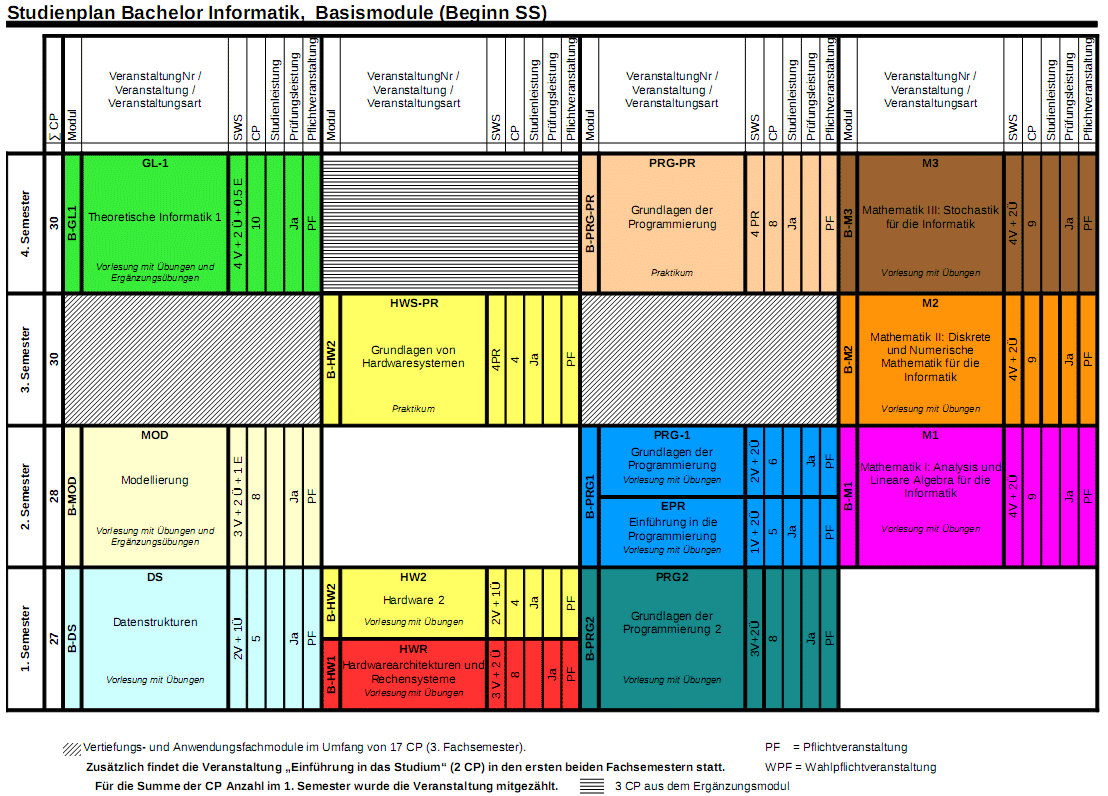
\includegraphics[width=18cm]{bitmaps/bachelor/basismodulebachelorSS}
\newline
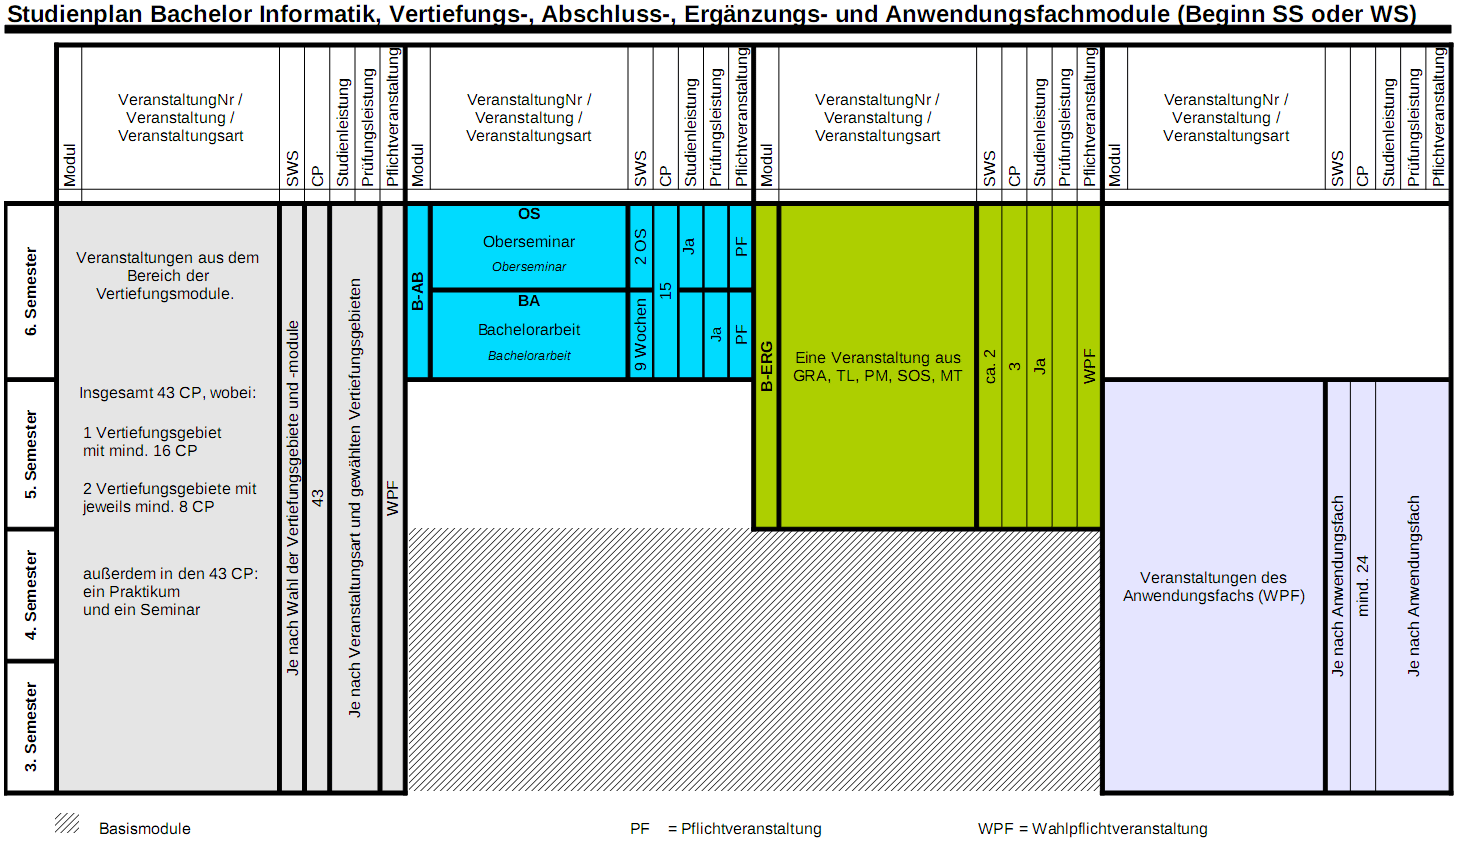
\includegraphics[width=18cm]{bitmaps/bachelor/sonstigemodulebachelor}
\newpage
\section{Der Bachelor Informatik - ein vollkommen verkorkstes Rollenspielsystem }
\spaltenanfang
Was ist eingendlich so ein Bachelor? Denn mein Englisch-Deutsch-W\"orterbuch
sagt, dass ich mich in einen Studiengang eingetragen habe, in dem ich zum
''Jungesellen der Rechner-Wissenschaft'' gemacht werden soll. Und der
Jungesellenstatus in der Wissenschaft kann nicht wirklich mein Ziel sein, oder?

Wie immer: Don't Panic! Bachelor ist nur ein Name, den die Politik \"ubernommen
hat, um internationaler zu klingen.  So ist das halt bei Hochschulreformen. Und
au{\ss}erdem ist was der Bachelor genau ist erst wichtig wenn ihr fertig seit.
Jetzt ist ersmal wichtig dass ihr sinnvoll studieren k\"onnt. Und dazu solltet
ihr ein paar Grundlagen wissen.

\textbf{Merke: Das Bachelorstudium ist im Prinzip ein verkorkstes Rollenspiel}

Als erstes gibt es f\"ur Rollenspielfanatiker und Munchkins das offizielle
Regelwerk zum Studium: Die \textsc{\textit{Bachelorordnung}}. Die besteht wie jedes
Regelwerk aus einem kleinen Teil mit Regeln
%TODO:*U NO SAY*
und dem Teil mit den riesigen
Tabellen, die Zeuch beschreiben. Aber anstatt coole R\"ustung und so gibt es
nur Skills. Nur hei{\ss}en die hier Module und man bekommt die erst, wenn man sie
verdient hat.

Ausserdem gibt es sowas wie XP. Die heissen hier aber CP, weil das alles
bitterer Ernst ist und sich deshalb nicht an g\"angige Rollenspiel
Designkonventionen gehalten wird. Und von denen bekommt man etwa einen pro 30
Stunden Studium.

Aber auch das funktioniert irgendwie anders als man das gewohnt ist. Statt dass
man XP bekommt, mit denen man sich bessere Skills holt um dann in Proben
bessere Chancen zu haben, muss man hier erst die Pr\"ufungen bestehen, bekommt
dann das Modul und damit die CP.
%TODO: *DAFU?*.

{\large
\begin{verbatim}
[XP] -> [skills] -> [pruefungen]
[CP] <- [module] <- [pruefungen]
\end{verbatim}}

\textbf{Bacheloraufbau:}
Schauen wir uns also das System mal genauer an.
Das Ziel ist es den Abschluss Bachelor zu bekommen. Dazu muss man 180CP
bekommen haben, die man mit dem Abschluss von Modulen bekommen hat. Und wie
jeder weiss, muss ein guter Munchkin Min-Maxen. Aber auch das kann der Bachelor
nicht gut.

Um Module abzuschlie\ss en muss man eine Klausur schreiben, eine m\"undliche
Pr\"ufung machen, einen Vortrag halten, gen\"ugend Abgaben gemacht haben, oder
sonst irgendwie gezeigt haben, dass man die CP auch wirklich verdient hat.


\textbf{Die Modulkategorien:}
Die Module sind wie f\"ur Skills \"ublich in verschiedene Kategorien
eingeteilt. Das kann euch sowohl einschr\"anken als auch Freiheiten geben.
Als erstes sind f\"ur euch die \emph{Basismodule} interessant, denn die m\"usst ihr als Informatiker alle machen.\\
Dann kommen die \emph{Vertiefungsmodule} ins Spiel. Hier kann man seinen Studenten in mindestens drei von f\"unf Kategorien spezialisieren.\\
Die \emph{Anwendungsfachmodule} sind Multiklassenskills, in denen ihr Fertigkeiten aus anderen F\"achern lernen sollt.\\
\emph{Erg\"anzungsmodule} sind durch die \texttt{Gute Idee\texttrademark} entstanden, dass Informatiker mindestens 150 Stunden Soft Skills oder soziales Zeuch gemacht haben sollten. Wir wollen doch keine verschrobenen antisozialen Studenten bauen.\\
Und zum Abschluss gibt es das \emph{Abschlussmodul}, das die Bachelorarbeit und das Oberseminar \"uber die Arbeiten enth\"alt.\\

\begin{center}
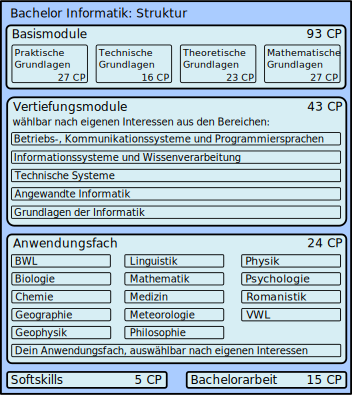
\includegraphics[width=85mm]{bilder/BacInfStruktur}
\end{center}


\textbf{Basismodule:}
Es gibt ein paar Skills die jeder Informatiker haben sollte. Und es gibt
Basismodule. In den Basismodulen lernt ihr offiziell vier Dinge: Mathe, Wie
Computer funktionieren (wird gerne auch ''Hardware'' genannt), Wie man Computer
programmiert und Theoretische Informatik. Das sind alles Vorlesungen, bis auf
das Programmier-Praktikum und das Hardware-Praktikum, die Praktika sind.
Insgesamt gibt es hier 93CP zu holen.

\textbf{Vertiefungsmodule:}
Die gibt es in f\"unf Spezialisierungen: BKSPP, ISWV, TS, ANI und GDI. \emph{''Betriebs-
und Kommunikationssysteme und Progammiersprachen und -paradigmen''} enth\"alt
genau was im Titel steht. \emph{''Informationssysteme und Wissensverarbeitung''}
besch\"aftigt sich mit Textverarbeitung , Datenbanken und k\"unstlicher
Intelligenz. In \emph{''Technische Systeme''} lernt man mehr \"uber Microcontroller,
Rechnerarchitektur und Chipdesign. \emph{''Angewandte Informatik''} ist alles was
sonst nicht untergebracht werden konnte. Da sind dann so Sachen wie
Computergrafik, Zeug und Krempel drin. Wer aber statt Zeug und Krempel lieber
was abgehobenes macht kann in \emph{''Grundlagen der Informatik''} fast schon ein
Mathestudium simulieren. Dort ist mehr Logik, mehr Algorithmentheorie und mehr
Beweise.

Und jetzt kommt der Haken: Du musst mindestens 43CP machen und davon in einem
mindestens 16CP und in zwei anderen mindestens 8CP und die anderen 11CP kannst
du machen wie du willst. Dabei musst du die drei Vertiefungsgebiete, in denen
du leveln willst, dem Pr\"ufungsamt vor der ersten Klausur mitteilen. Alles
Klar? OK!

\textbf{Anwendungsfachmodule:}
Die Muliklassenskills auch Anwendungsfachmodule genannt erlauben euch was anderes als Informatik zu lernen.
Die mei{\ss}ten dieser Nebenfachmodule sind geregelt. Das hei{\ss}t das
Basisregelwerk ''Die Bachelorordnung'' hat vorgefertigte L\"osungen wie ihr das
Nebenfach machen k\"onnt. Ist euer Nebenfach nicht drin, k\"onnt ihr das trotzdem studieren, aber dann halt ungeregelt.
Dazu muss unser Pr\"ufungsamt mit dem ''gegnerischen'' Pr\"ufungsamt ''kl\"aren'' wie das ganze abgewickelt werden soll.
Fakt ist aber, ihr braucht immer mindestens 24CP.

\textbf{Erg\"anzungsmodule:}
Irgendein schlauer Informatiker hat sich mal gedacht: \emph{Wir wollen, das
Frankfurter Informatiker nicht nur Fachidioten sind, sondern auch ''sozial''
sein k\"onnen. Die haben dann ''Soft Skills''. Wie ''Teamf\"ahigkeit'' und so. Und das
ist dann gut.} Aber da zu viel Soziales nicht in den Studienverlausplan passt, macht ihr 5CP.
Da ist dann auch die Studienorientierung STO drin. Die im ersten Semester 2CP gibt, und sp\"ater nur noch halb so viel.
Da wird euch nochmal wie man studiert auf dem Silbertablett gereicht.

\textbf{Die restlichen 15CP:}
Gibt es mit der Bachlorarbeit.

\textbf{Die Bachelorarbeit:}
Das ist sowas wie eine echte wissenschaftliche Arbeit. Wenn ihr die gamcht habt gibt das 15CP im Abschlussmodul.

\begin{center}
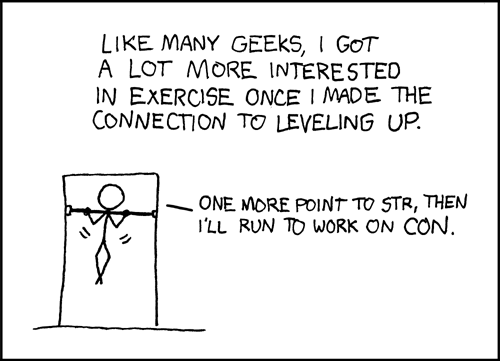
\includegraphics[width=\linewidth]{comics/exercise}\\
\end{center}

\textbf{Die Klausurregeln:}
Und nun steigt die Spannung. Die Klausurphase beginnt.
W\"ahrend im Semester Wochen vergehen k\"onnen, ohne das viel passiert, ist die Klausurphase eher wie Kampfrunden.
Eine Megasekunde, die im echten Leben vergehet, kommt einem wie eine Gigasekunde an der Uni vor.
    Aber keine Panik, es gibt einige Tricks und ein paar Regeln, die ihr
anwenden k\"onnt, um sinnvoll lebendig, und mit ein paar mehr CP durch die
Klausurphase zu kommen.

\textbf{Anmeldung:}
Zu Klausuren m\"usst ihr euch zwei Wochen vorher angemeldet haben. Und vor der ersten Klausur m\"usst ihr euch f\"ur den Bachlor anmelden.
Wenn ihr die Klausur schreibt und nicht angemeldet seit, gibt das keine XCP

\textbf{Timing:}
Zuerst ist wichtig zu planen wann ihr Klausuren schreibt.
Die Termine selbst k\"onnt ihr zwar nicht \"andern, aber ein guter Munchkin hat die Bachelorordnung gelesen
und hat festgestellt, dass viele Klausuren jedes Semester angeboten werden.

Aber wie soll es mir helfen die Klausur zu verschieben?
N\"achstes Semsester sind doch wieder Klausuren, oder?

Aber da ist es wichtig
zu wissen, wie die Professoren diese Regel mit jedem Semester auslegen.
Professoren waren alle mal Studenten und sind deshalb fast so faul wie wir.
Und fast immer m\"ussen Nachklausuren angeboten werden, f\"ur Studenten, die durchgefallen sind oder nicht teilnehmen konnten.
W\"ahrend die Vorlesungen meisstens in der dritten April- oder Oktoberwoche anfangen f\"angt das Semester p\"unklich am Ersten an.

Und deshalb sind die Nachklausuren mei{\ss}tens am Ende der Semesterferien, aber im neuen Semester. Der
ge\"ubte Munchkin braucht also seine Klausuren nicht alle auf einmal zu
schreiben, sondern lernt am Anfang \emph{und} am Ende der Semesterferien.
Ansonsten gilt: \textbf{Konzentrier dich auf wenige Klausuren, statt in allen zu versagen.}
\emph{Bla, bla, lernt rechtzeitig, bla\dots}\\

\textbf{Freiversuche - Rerolls f\"ur Klausuren:}
Und jetzt kommen die kleinen Feinheiten des Regelwerks die jeden Munchkin interessieren sollten.
Ger\"uchteweise haben manche Studenten Klausuren mitgeschrieben und kl\"aglich versagt. Daran ist noch nichts besonderes.
Aber die f\"ur diese Studenten war es so als h\"atten sie die Klausur nie
geschrieben und haben sich einfach beim n\"achsten mal wieder in die Klausur
gesetzt. Und noch viel besser. Andere die grad so bestanden hatten, sa{\ss}en
in der Klausur und konnnten nochmal mitschreiben und haben am Ende eine bessere
Note gehabt. Wie geht das?

Naja, eigendlich ist nichts besonderes daran. Wenn du innerhalb der
Freiversuchsfrist eine Klausur schreibst, kannst du beim ersten Mal
Durchfallen, ohne dass das als Fehlversuch gez\"ahlt wird.
Die Freiversuchsfrist ist in der Bachelorordnung festgelegt und ist an den Studienverlauf angepasst.
Das soll euch dazu motivieren die Klausur zu beim erstem Mal oder in der Nachklausur mitzuschreiben.
Das funktioniert aber nur in den Basismodulen so. In den Vertiefungs und Anwendungsfachmodulen funktioniert das leider nicht.
Aber die Basismodule machen \"uber die H\"alfte des Studiums aus, also ist das gar nicht so schlecht.

Und wer wider erwarten die Klausur besteht und mit seiner Note nicht zufrieden
ist, kann die Klausur nochmal schreiben. Dazu muss man sich nach der Klausur
f\"ur die n\"achste Klausur anmelden. Das kann man aber auch nur in den
Basismodulen und insgesamt nur f\"unf mal. Da es aber nur 9 Klausuren in den Basismodulen gibt,
ist das immer noch viel. Aber die genauen Regeln bekommt ihr noch rechtzeitig in der Studienorientierung erz\"ahlt.

\textbf{Studienorientierung:}
\textbf{
Die Studienorientierung ist soooo wichig dass wir einen extra Artikel geschrieben haben. Macht die im ersten Semester und alles wird gut. Ausserdem haben wir diesen Absatz extra fettgedruckt!}

\textbf{FAIL - Das Howto:}
Manchmal muss man einfach alle Br\"ucken hinter sich lassen. Und manchmal will man nicht gehen, sondern rausfliegen. Und so gehts:

\textbf{FAIL - Die Sparsame Methode:}
Bezahl deine Studiengeb\"uhren nicht. So einfach ist das. Die bezahlt man sonst immer im Januar oder im Juli. Aber wer wirklich raus will findet in der Sparsamkeit eine wirksame Methode.

\textbf{FAIL - Die Faule Methode:}
Mach in den ersten drei Semestern weniger als 15CP. Das sind so ungef\"ahr zwei Module von zehn. Dann musst du nur noch die Anfragen vom Pr\"ufungsamt ignorieren und keine Fristverl\"angerung beantragen. Dann bist du raus.

\textbf{ULTRAFAIL - Die Wahre Methode:}
Wenn du nicht nur rausfliegen willst, sondern gar nicht mehr Informatik
studieren k\"onnen willst, solltest du dreimal durch eine Pr\"ufung in einem
Basismodul durchfallen (viermal, wenn du schon in der Freiversuchsfrist
anf\"angst). Wer eine Pr\"ufung dreimal nicht besteht, hat ''endg\"ultig nicht
bestanden''. Und wenn das soetwas grundlegendes wie Programmierung ist, kannst
du nicht mehr Informatik studieren, auch nicht woanders in Deutschland. Auch
hier musst du darauf achten alle Beratungsgespr\"ache zur\"uckzuweisen.

\textbf{N\"utzliche Tips:}
\emph{bla, bla, \"Ubungsabgaben, yadda, yadda, Lernen, bla, blubber, Zeiteinteilung, bla, regelm\"a{\ss}ig da sein, trololo, Durchhalteverm\"ogen, bla, generische Motivationsrede\dots}\\

\textbf{Und nun?}
Naja, da sind noch mehr Seiten in der Don't Panic! 42. Die k\"onnt ihr auch
lesen. Wichtig ist vor allem sich an der Uni einzuleben, wenn man erfolgreich
studieren will. Und das sieht f\"ur jeden anders aus. Manche machen ihr Studium
schnell und andere lassen sich Zeit. Und wichtiger als die Skills, die ihr hier
bekommt, ist die Erfahrung. Wenn ihr hier fertig seit, m\"usst ihr eh wieder
neue Sachen lernen.






\spaltenende
\begin{center}
	\vspace{1cm}
	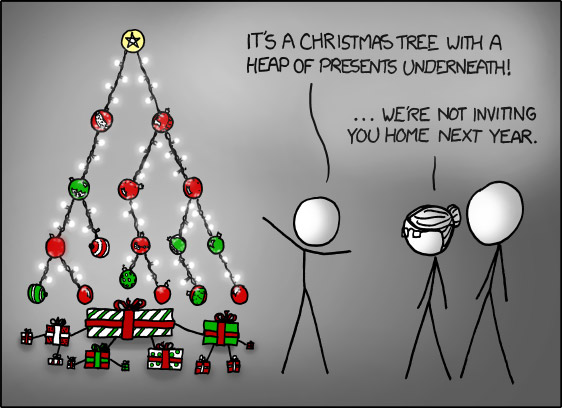
\includegraphics[scale=0.63]{comics/tree}
\end{center}
\newpage

%%%%%%%%%%%%%%%%%%%%%%%%%%%%%%%%%%%%%%%%%%%%%%%%%%%%%%%%%%%%%%%%%%%%%%%%%%%5

%\section{Prüfungsanmeldung Bachelor HOW-TO}
%\spaltenanfang
%Irgendwann im Verlauf des ersten Semesters werdet ihr euch für die ersten Prüfungen anmelden. Damit ihr nicht in Zeitnot bei der Anmeldung geratet, hier ein kleiner Überblick wie ihr euch für welche Prüfungen anmeldet.

Schriftliche Modulabschlussprüfungen: Im ersten Semester werden die Modulabschlussprüfungen, die ihr machen werdet, wohl B-M1 (Lineare Algebra und Analysis für Informatiker) und B-MOD sein (Diskrete Modellierung). Allerspätestens vier Wochen vor dem Klausurtermin müsst ihr im Prüfungsamt den entsprechenden Zettel ausgefüllt abgeben. Da im Prüfungsamt der Betrieb kurz vor den Klausuren ziemlich hoch ist, sollte man sich früh genug um die Anmeldung kümmern und nicht erst am letztmöglichen Tag. Damit ihr aber überhaupt an eurer ersten Modulabschlussprüfung teilnehmen könnt, müsst ihr zuvor die Zulassung zur Bachelorprüfung beantragen. Zulassung zur Bachelorprüfung: Folgendes müsst ihr hierfür im Prüfungsamt abgeben:
\begin{itemize}
\item Immatrikulationsbescheinigung
\item Schriftliche Erklärung zur evtl. Immatrikulation in verwandten Studiengängen.
%\item Nachweis über die Zahlung der Prüfungsgebühr ( 75 \euro{})
\item Nachweise zu Studien- und Prüfungsleistungen für die eine Anrechnung begehrt wird
\item ggf. Erklärung, falls man einen Nachteilsausgleich gemäß § 21 in Anspruch nehmen will
\end{itemize}
Anmeldung für Studienleistungen: Im ersten Semester werdet ihr aller Wahrscheinlichkeit nach mit den Klausuren in PRG-1 und EDGI Studienleistungen erwerben, wenn ihr eben diese besteht. Die Informationen für die Anmeldung zur jeweiligen Klausur werden in der jeweiligen Vorlesung bekannt gegeben. Anmeldung zu einer mündlichen Modulabschlussprüfung: Für die mündliche Modulabschlussprüfung meldet ihr euch genauso an, wie für die schriftliche Modulabschlussprüfung. Also vier Wochen vorher das entsprechende Formular ausgefüllt abgeben. Damit ihr euch aber für eine mündliche Modulabschlussprüfung anmelden könnt, müsst ihr euch zunächst einen Termin beim dem Professor, der euch prüfen soll, holen. Dieser Professor muss euch dann auch das Formular unterschreiben. In Modulen, in denen die Vorlesung von mehreren Professoren gehalten wurde, wie z.B. in B-PRG könnt ihr euch einen Prüfer aussuchen. Da auch Professoren manchmal Urlaub machen, solltet ihr euch die Prüfungstermine rechtzeitig besorgen. Wenn ihr all diese Hürden für die Anmeldung gemeistert habt, bleibt nur noch eins: Viel Erfolg und Don‘t Panic!

\begin{flushright}Tim und Claudia\end{flushright}

%\spaltenende

%%%%%%%%%%%%%%%%%%%%%%%%%%%%%%%%%%%%%%%%%%%%%%%%%%%%%%%%%%%%%%%%%%%%%%%%%%%5

\section{Master - was ist das?}
\spaltenanfang
Nachdem du es also gepackt hast, einen Bachelor mit einer Note von nicht schlechter als 3.0 zu erwerben, hast du dich für den Masterstudiengang an der Goethe-Universität Frankfurt entschieden.


Da die Ordnung für Studienanfänger im Masterstudiengang aber etwas verwirrend sein kann, gibt es dazu hier einige Erläuterungen.


Zunächst sollte bemerkt werden, das du dich entscheiden musst, was für einen Master du letztendlich machen willst, denn der Master in Informatik ist unterteilt in vier Schwerpunkte:
\begin{noindEnumerate}
\item Master mit Anwendungsfach
\item Master mit vertieftem Anwendungsfach
\item Master in allgemeiner Informatik
\item Master mit Spezialisierung
\end{noindEnumerate}

Hierzu sei gesagt, dass wenn du im Bachelor kein Anwendungsfach studiert hattest, du keine andere Möglichkeit hast, als den Master mit Anwendungsfach zu machen.


Hattest du hingegen im Bachelorstudium schon ein Anwendungsfach belegt, so kannst du nun ein neues Anwendungsfach belegen, das alte Anwendungsfach vertiefen oder dich zwischen dem Master in allgemeiner Informatik und dem Master mit Spezialisierung entscheiden, falls du dich gegen ein Anwendungsfach entscheidest.


Kommst du von einer anderen Universität und hast deinen Bachelor nicht an der Universität Frankfurt abgelegt, so kann es sein, das du Auflagen erteilt bekommst oder die Wahl des Schwerpunktes eingeschränkt wird. Die Vorlesungen, die du als Auflagen erteilt bekommst und die nicht mehr als 30 CP umfassen, musst du dann innerhalb von 14 Monaten erfolgreich abschließen.


Insgesamt geht das Masterstudium über vier Semester und besteht aus 120 CP. Egal für welche dieser vier Formen des Masterstudiums du dich entscheidest, am Ende musst du bei allen im Abschlussmodul eine Masterarbeit schreiben, die 30 CP bringt und gewöhnlich über ein Semester geht (6 Monate).


Die Informatikmodule sind in drei Gebiete aufgeteilt: „Informatik der Systeme“, „Grundlagen der Informatik“ und „Angewandte Informatik“. Je nach gewähltem Schwerpunkt musst du aus jedem der Gebiete eine bestimmte Anzahl an CP erbringen. Unter den Informatikmodulen muss jedoch mindestens ein Seminar und ein Praktikum sein.


Zusätzlich sind in jedem Schwerpunkt Ergänzungsmodule zu belegen, die 3 bis 6~CP bringen. Bei diesem Ergänzungsmodul handelt es sich um Veranstaltungen wie „Tutoriumsleitung“, die Vorlesungen „IT-Projektmanagement“ und „Neue Medien und Gesellschaft“. Desweiteren gehört das Modul „Soft Skills“ noch zu den Ergänzungsmodulen. In diesem Modul können im entsprechenden Umfang Veranstaltungen gewählt werden, die wissenschaftliches Arbeiten, Präsentationstechniken, Themen aus dem Bereich „Informatik und Gesellschaft“ und Wissensethik und weitere Soft Skills vermitteln. Diese Veranstaltungen werden nicht unbedingt vom Institut für Informatik angeboten, sondern auch z.B. vom Didaktischen Zentrum der Uni. 


\spaltenende

\begin{figure}[bt]
\begin{center}
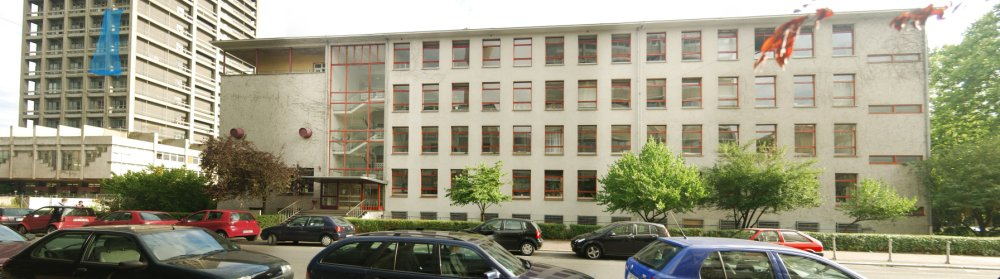
\includegraphics[scale=1.0]{fotos/rm_pano}
\end{center}
\end{figure}

%%%%%%%%%%%%%%%%%%%%%%%%%%%%%%%%%%%%%%%%%%%%%%%%%%%%%%%%%%%%%%%%%%%%%%%%%%%5
% HINWEIS: vspace braucht man als Workaround beim geometry-Package, da LaTeX den Grafiken sonst nicht genug Platz in der Vertikalen einräumt.
%%%%%%%%%%%%%%%%%%%%%%%%%%%%%%%%%%%%%%%%%%%%%%%%%%%%%%%%%%%%%%%%%%%%%%%%%%%5

\subsection{Schwerpunkt: Allgemeine Informatik (120 CP)}

\vspace{-2mm}
\begin{addmargin}[0.8cm]{0cm}

\setlength{\unitlength}{1cm}
\setlength{\fboxrule}{1.25pt}
%\setlength{\fboxsep}{0pt}

\begin{picture}(16,7.4)


\definecolor{topinnerboxcolor}{rgb}{0.68, 0.84, 0.47}
\definecolor{leftinnerboxcolor}{rgb}{0.8, 0.97, 0.97}
\definecolor{middleinnerboxcolor}{rgb}{1.0, 1.0, 0.7}
\definecolor{rightinnerboxcolor}{rgb}{0.8, 0.8, 0.97}
\definecolor{topboxcolor}{rgb}{0.6, 0.70, 0.4}
\definecolor{sideboxgray}{gray}{0.9}

%linke Seitenbox
\put(0.5,1.2){\fcolorbox{black}{white}{\makebox(2.7,6)[l]{ } }  }
\put(0.85,2.2){\fcolorbox{black}{sideboxgray}{\makebox(2,4)[l]{ } }  }

%mittlere Box
\put(4.4,1.2){\fcolorbox{black}{white}{\makebox(8.0,6)[l]{ } }  }
\put(4.6,2.2){ \fcolorbox{black}{leftinnerboxcolor}{ \makebox(2,3.15)[l]{ } }  }
\put(7.2,2.2){ \fcolorbox{black}{middleinnerboxcolor}{ \makebox(2,3.15)[l]{ } }  }
\put(9.8,2.2){ \fcolorbox{black}{rightinnerboxcolor}{ \makebox(2,3.15)[l]{ } }  }
\put(4.6,5.6){ \fcolorbox{black}{topinnerboxcolor}{ \makebox(7.2, 0.6)[l]{ } }  }

%rechte Seitenbox
\put(13.5,1.2){\fcolorbox{black}{white}{\makebox(2.7,6)[l]{ } }  }
\put(13.85,2.2){\fcolorbox{black}{sideboxgray}{\makebox(2,4)[l]{ } }  }


%%%%%%%%%%%%%%%%%%%%%%%%%%%%%%%%%%%%%%%%%%%%%%%%%%%%%%%%%%%%%%%%%%%%%%%%%%%%%


%Nebenbeschriftung
\put(0.97,6.7){\textsf{Masterarbeit}}
\put(14.0,6.9){\textsf{Ergänzungs-}}
\put(14.4,6.5){\textsf{module}}
\put(1.5,4.2){\textsf{30 CP}}
\put(14.5,4.2){\textsf{3-6 CP}}

%Hauptbeschriftung
\put(7.55,6.7){\textsf{Informatik$^{1,2}$}}
\put(5.23,5.75){ \textsf{\textbf{24-27 CP} frei aus allen drei Gebieten}}

\put(5.5,4.2){\textsf{20 CP}}
\put(5.15,3.1){\scriptsize \textsf{Informatik der}}
\put(5.48,2.7){\scriptsize \textsf{Systeme}}

\put(8.05,4.2){\textsf{20 CP}}
\put(7.65,3.1){\scriptsize \textsf{Grundlagen der}}
\put(7.95,2.7){\scriptsize \textsf{Informatik}}

\put(10.65,4.2){\textsf{20 CP}}
\put(10.45,3.1){\scriptsize \textsf{Angewandte}}
\put(10.55,2.7){\scriptsize \textsf{Informatik}}

\put(7.1,1.45){\textsf{Summe: 84-87 CP}}

%Fussnoten
\put(1.0,0.4){\scriptsize \textsf{1) Maximal 27 CP aus den einführenden Modulen}}
\put(1.0,0.1){\scriptsize \textsf{2) Muss mindestens ein Praktikum und ein Seminar aus der Informatik enthalten}}

\end{picture}

\end{addmargin}

\spaltenanfang
Bei diesem Schwerpunkt wirst du, wie der Name schon sagt, fast nur Informatikveranstaltungen besuchen. An Informatikmodulen musst du insgesamt mindestens 84 CP erwerben. Davon aus jedem der drei Gebiete mindestens 20 CP. Dabei kannst du maximal 27 CP aus den einführenden Modulen belegen. Die restlichen CP kannst du frei wählen.
\spaltenende

\subsection{Schwerpunkt: Informatik mit Anwendungsfach (120 CP)}

\vspace{6mm}
\begin{addmargin}[-3mm]{5cm}

\setlength{\unitlength}{1cm}
\setlength{\fboxrule}{1.25pt}

\begin{picture}(18,8)


\definecolor{topinnerboxcolor}{rgb}{0.68, 0.84, 0.47}
\definecolor{leftinnerboxcolor}{rgb}{0.8, 0.97, 0.97}
\definecolor{middleinnerboxcolor}{rgb}{1.0, 1.0, 0.7}
\definecolor{rightinnerboxcolor}{rgb}{0.8, 0.8, 0.97}
\definecolor{topboxcolor}{rgb}{0.6, 0.70, 0.4}
\definecolor{sideboxgray}{gray}{0.9}

%linke Seitenbox
\put(0.5,2.4){\fcolorbox{black}{white}{\makebox(2.7,6)[l]{ } }  }
\put(0.85,3.4){\fcolorbox{black}{sideboxgray}{\makebox(2,4)[l]{ } }  }

%Aussenrahmen
\put(4.1,1.4){\fcolorbox{black}{white}{\makebox(10.6,7.3)[l]{ } }  }

%mittlere Box
\put(4.4,2.4){\fcolorbox{black}{white}{\makebox(6.5,6)[l]{ } }  }
\put(4.6,3.4){ \fcolorbox{black}{leftinnerboxcolor}{ \makebox(1.5,3.15)[l]{ } }  }
\put(6.7,3.4){ \fcolorbox{black}{middleinnerboxcolor}{ \makebox(1.5,3.15)[l]{ } }  }
\put(8.8,3.4){ \fcolorbox{black}{rightinnerboxcolor}{ \makebox(1.5,3.15)[l]{ } }  }
\put(4.6,6.8){ \fcolorbox{black}{topinnerboxcolor}{ \makebox(5.7, 0.6)[l]{ } }  }

%Sonderbox
\put(11.7,2.4){\fcolorbox{black}{white}{\makebox(2.7,6)[l]{ } }  }
\put(12.05,3.4){\fcolorbox{black}{sideboxgray}{\makebox(2,4)[l]{ } }  }

%rechte Seitenbox
\put(15.5,2.4){\fcolorbox{black}{white}{\makebox(2.7,6)[l]{ } }  }
\put(15.85,3.4){\fcolorbox{black}{sideboxgray}{\makebox(2,4)[l]{ } }  }


%%%%%%%%%%%%%%%%%%%%%%%%%%%%%%%%%%%%%%%%%%%%%%%%%%%%%%%%%%%%%%%%%%%%%%%%%%%%%


%Nebenbeschriftung
\put(0.97,7.9){\textsf{Masterarbeit}}
\put(1.5,5.4){\textsf{30 CP}}

\put(15.97,8.1){\textsf{Ergänzungs-}}
\put(16.39,7.7){\textsf{module}}
\put(16.48,5.4){\textsf{3-6 CP}}

%Sonderboxbeschriftung
\put(11.85,7.9){\small \textsf{Anwendungsfach$^3$}}
\put(12.5,5.4){\textsf{24-27 CP}}

%Hauptbeschriftung
\put(6.83,7.9){\textsf{Informatik$^{1,2}$}}
\put(5.1,7.0){\footnotesize \textsf{\textbf{12-15 CP} frei aus allen drei Gebieten}}

\put(5.21,5.4){\textsf{16 CP}}
\put(4.9,4.3){\scriptsize \textsf{Informatik der}}
\put(5.23,3.9){\scriptsize \textsf{Systeme}}

\put(7.31,5.4){\textsf{16 CP}}
\put(6.91,4.3){\scriptsize \textsf{Grundlagen der}}
\put(7.23,3.9){\scriptsize \textsf{Informatik}}

\put(9.41,5.4){\textsf{16 CP}}
\put(9.21,4.3){\scriptsize \textsf{Angewandte}}
\put(9.31,3.9){\scriptsize \textsf{Informatik}}

\put(6.55,2.7){\textsf{Summe: 60 CP}}
\put(8.1,1.7){\textsf{Summe: 84-87 CP}}

%Fussnoten
\put(1.0,0.7){\scriptsize \textsf{1) Maximal 27 CP aus den einführenden Modulen}}
\put(1.0,0.4){\scriptsize \textsf{2) Muss mindestens ein Praktikum und ein Seminar aus der Informatik enthalten}}
\put(1.0,0.1){\scriptsize \textsf{3) Muss verschieden von einem bereits im vorangegangenen Bachelorstudiengang studierten Anwendungsfach sein}}

\end{picture}

\end{addmargin}

\spaltenanfang
Belegst du den Schwerpunkt „Informatik mit Anwendungsfach“, so brauchst du nur mindestens 60~CP aus den Informatikmodulen. Dabei müssen jeweils mindestens 16 CP in den drei Gebieten belegt werden. Maximal 27 CP kannst du aus den einführenden Modulen wählen. Die restlichen CP sind auch auch hier wieder frei wählbar. Aus dem Anwendungsfach müssen mindestens 24 CP eingebracht werden. Du kannst dein Anwendungsfach aus folgenden Fächern wählen: Linguistik, Physik, Philosophie, Biologie, Geographie, Meteorologie, Mathematik, Geophysik, Chemie, Medizin, VWL, BWL und Romanistik. Dabei musst du beachten, dass du dieses Anwendungsfach noch nicht im Bachelor mit eingebracht haben darfst. Andere Fächer sind auf Antrag auch möglich.

\spaltenende

\subsection{Schwerpunkt: Informatik mit vertieftem Anwendungsfach (120 CP)}

\vspace{10mm}
\begin{addmargin}[-3mm]{0cm}

\setlength{\unitlength}{1cm}
\setlength{\fboxrule}{1.25pt}

\begin{picture}(18,8)


\definecolor{topinnerboxcolor}{rgb}{0.68, 0.84, 0.47}
\definecolor{leftinnerboxcolor}{rgb}{0.8, 0.97, 0.97}
\definecolor{middleinnerboxcolor}{rgb}{1.0, 1.0, 0.7}
\definecolor{rightinnerboxcolor}{rgb}{0.8, 0.8, 0.97}
\definecolor{topboxcolor}{rgb}{0.6, 0.70, 0.4}
\definecolor{sideboxgray}{gray}{0.9}

%linke Seitenbox
\put(0.5,2.4){\fcolorbox{black}{white}{\makebox(2.7,6)[l]{ } }  }
\put(0.85,3.4){\fcolorbox{black}{sideboxgray}{\makebox(2,4)[l]{ } }  }

%Aussenrahmen
\put(4.1,1.4){\fcolorbox{black}{white}{\makebox(10.6,7.3)[l]{ } }  }

%mittlere Box
\put(4.4,2.4){\fcolorbox{black}{white}{\makebox(6.5,6)[l]{ } }  }
\put(4.6,3.4){ \fcolorbox{black}{leftinnerboxcolor}{ \makebox(1.5,3.15)[l]{ } }  }
\put(6.7,3.4){ \fcolorbox{black}{middleinnerboxcolor}{ \makebox(1.5,3.15)[l]{ } }  }
\put(8.8,3.4){ \fcolorbox{black}{rightinnerboxcolor}{ \makebox(1.5,3.15)[l]{ } }  }
\put(4.6,6.8){ \fcolorbox{black}{topinnerboxcolor}{ \makebox(5.7, 0.6)[l]{ } }  }

%Sonderbox
\put(11.7,2.4){\fcolorbox{black}{white}{\makebox(2.7,6)[l]{ } }  }
\put(12.05,3.4){\fcolorbox{black}{sideboxgray}{\makebox(2,4)[l]{ } }  }

%rechte Seitenbox
\put(15.5,2.4){\fcolorbox{black}{white}{\makebox(2.7,6)[l]{ } }  }
\put(15.85,3.4){\fcolorbox{black}{sideboxgray}{\makebox(2,4)[l]{ } }  }


%%%%%%%%%%%%%%%%%%%%%%%%%%%%%%%%%%%%%%%%%%%%%%%%%%%%%%%%%%%%%%%%%%%%%%%%%%%%%


%Nebenbeschriftung
\put(0.97,7.9){\textsf{Masterarbeit}}
\put(1.5,5.4){\textsf{30 CP}}

\put(15.97,8.1){\textsf{Ergänzungs-}}
\put(16.39,7.7){\textsf{module}}
\put(16.48,5.4){\textsf{3-6 CP}}

%Sonderboxbeschriftung
\put(12.47,8.1){\textsf{vertieftes$^3$}}
\put(11.83,7.7){\textsf{Anwendungsfach}}
\put(12.5,5.4){\textsf{24-27 CP}}

%Hauptbeschriftung
\put(6.83,7.9){\textsf{Informatik$^{1,2}$}}
\put(5.1,7.0){\footnotesize \textsf{\textbf{12-15 CP} frei aus allen drei Gebieten}}

\put(5.21,5.4){\textsf{16 CP}}
\put(4.9,4.3){\scriptsize \textsf{Informatik der}}
\put(5.23,3.9){\scriptsize \textsf{Systeme}}

\put(7.31,5.4){\textsf{16 CP}}
\put(6.91,4.3){\scriptsize \textsf{Grundlagen der}}
\put(7.23,3.9){\scriptsize \textsf{Informatik}}

\put(9.41,5.4){\textsf{16 CP}}
\put(9.21,4.3){\scriptsize \textsf{Angewandte}}
\put(9.31,3.9){\scriptsize \textsf{Informatik}}

\put(6.55,2.7){\textsf{Summe: 60 CP}}
\put(8.1,1.7){\textsf{Summe: 84-87 CP}}

%Fussnoten
\put(1.0,0.7){\scriptsize \textsf{1) Maximal 27 CP aus den einführenden Modulen}}
\put(1.0,0.4){\scriptsize \textsf{2) Muss mindestens ein Praktikum und ein Seminar aus der Informatik enthalten}}
\put(1.0,0.1){\scriptsize \textsf{3) Das gleiche Anwendungsfach muss bereits als Anwendungsfach im vorangegangenen Bachelorstudiengang studiert worden sein}}

\end{picture}

\end{addmargin}

\spaltenanfang
Bei dem Schwerpunkt „Informatik mit vertieftem Anwendungsfach“ kannst du ein Anwendungsfach vertiefen, das du bereits im Bachelorstudium belegt hast. Bisher sind Mathematik, Geographie, Geophysik, Linguistik, Philosophie und Medizin geregelt. Aus diesem vertieften Anwendungsfach musst du mindestens 24~CP belegen. In den Informatikmodulen musst du insgesamt mindestens 60 CP belegen, wobei aus jedem der drei Gebiete mindestens 16~CP eingebracht werden müssen. Dabei kannst du maximal 27 CP aus den einführenden Modulen belegen. Der Rest ist auch hier wieder frei wählbar.

\spaltenende

\subsection{Schwerpunkt: Informatik mit Spezialisierung (120 CP)}

\vspace{10mm}
\begin{addmargin}[-3mm]{0cm}

\setlength{\unitlength}{1cm}
\setlength{\fboxrule}{1.25pt}

\begin{picture}(18,8.5)


\definecolor{topinnerboxcolor}{rgb}{0.68, 0.84, 0.47}
\definecolor{leftinnerboxcolor}{rgb}{0.8, 0.97, 0.97}
\definecolor{middleinnerboxcolor}{rgb}{1.0, 1.0, 0.7}
\definecolor{rightinnerboxcolor}{rgb}{0.8, 0.8, 0.97}
\definecolor{topboxcolor}{rgb}{0.6, 0.70, 0.4}
\definecolor{sideboxgray}{gray}{0.9}

%linke Seitenbox
\put(0.5,2.7){\fcolorbox{black}{white}{\makebox(2.7,6)[l]{ } }  }
\put(0.85,3.7){\fcolorbox{black}{sideboxgray}{\makebox(2,4)[l]{ } }  }

%Aussenrahmen
\put(4.1,1.7){\fcolorbox{black}{white}{\makebox(10.6,7.3)[l]{ } }  }

%mittlere Box
\put(4.4,2.7){\fcolorbox{black}{white}{\makebox(6.5,6)[l]{ } }  }
\put(4.6,3.7){ \fcolorbox{black}{leftinnerboxcolor}{ \makebox(1.5,3.15)[l]{ } }  }
\put(6.7,3.7){ \fcolorbox{black}{middleinnerboxcolor}{ \makebox(1.5,3.15)[l]{ } }  }
\put(8.8,3.7){ \fcolorbox{black}{rightinnerboxcolor}{ \makebox(1.5,3.15)[l]{ } }  }
\put(4.6,7.1){ \fcolorbox{black}{topinnerboxcolor}{ \makebox(5.7, 0.6)[l]{ } }  }

%Sonderbox
\put(11.7,2.7){\fcolorbox{black}{white}{\makebox(2.7,6)[l]{ } }  }
\put(12.05,3.7){\fcolorbox{black}{sideboxgray}{\makebox(2,4)[l]{ } }  }

%rechte Seitenbox
\put(15.5,2.7){\fcolorbox{black}{white}{\makebox(2.7,6)[l]{ } }  }
\put(15.85,3.7){\fcolorbox{black}{sideboxgray}{\makebox(2,4)[l]{ } }  }


%%%%%%%%%%%%%%%%%%%%%%%%%%%%%%%%%%%%%%%%%%%%%%%%%%%%%%%%%%%%%%%%%%%%%%%%%%%%%


%Nebenbeschriftung
\put(0.97,8.2){\textsf{Masterarbeit}}
\put(1.5,5.7){\textsf{30 CP}}

\put(15.97,8.4){\textsf{Ergänzungs-}}
\put(16.39,8.0){\textsf{module}}
\put(16.48,5.7){\textsf{3-6 CP}}

%Sonderboxbeschriftung
\put(11.95,8.2){\textsf{Spezialisierung$^3$}}
\put(12.75,5.7){\textsf{24 CP}}

%Hauptbeschriftung
\put(6.88,8.2){\textsf{Informatik$^1$}}
\put(5.1,7.3){\footnotesize \textsf{\textbf{12-15 CP} frei aus allen drei Gebieten}}

\put(5.21,5.7){\textsf{16 CP}}
\put(4.9,4.6){\scriptsize \textsf{Informatik der}}
\put(5.23,4.2){\scriptsize \textsf{Systeme}}

\put(7.31,5.7){\textsf{16 CP}}
\put(6.91,4.6){\scriptsize \textsf{Grundlagen der}}
\put(7.23,4.2){\scriptsize \textsf{Informatik}}

\put(9.41,5.7){\textsf{16 CP}}
\put(9.21,4.6){\scriptsize \textsf{Angewandte}}
\put(9.31,4.2){\scriptsize \textsf{Informatik}}

\put(6.55,3.0){\textsf{Summe: 60 CP}}
\put(8.1,2.0){\textsf{Summe: 84-87 CP$^2$}}

%Fussnoten
\put(1.0,1.0){\scriptsize \textsf{1) Maximal 27 CP aus den einführenden Modulen}}
\put(1.0,0.7){\scriptsize \textsf{2) Muss mindestens ein Praktikum und ein Seminar aus der Informatik enthalten}}
\put(1.0,0.4){\scriptsize \textsf{3) Mögliche Spezialisierungen sind:}}
\put(1.0,0.1){\tiny \textsf{Visual Computing, Complex Software Systems, Internet Computing, Design and Analysis of Algorithms, System Engineering, Knowledge Processing, Systems Science, Computational Science}}

\end{picture}

\end{addmargin}

\spaltenanfang
Bei dem Schwerpunkt „Informatik mit Spezialisierung“ könnt ihr unter den folgenden Spezialisierungen wählen:
\begin{noindItemize}
\item Visual Computing
\item Complex Software Systems
\item Internet Computing
\item Design and Analysis of Algorithms
\item Systems Engineering
\item  Knowledge Processing und Systems Science
\end{noindItemize}

Zunächst musst du hier auch Informatikmodule im Umfang von 60 CP belegen, wobei auch hier wieder aus jedem der drei Bereiche mindestens 16 CP eingebracht werden müssen. Die restlichen CP sind frei wählbar.

Zusätzlich müssen noch 24 CP zur gewählten Spezialisierung belegt werden. Welche Veranstaltungen zu einem Spezialisierungsgebiet gehören, kann der Übersicht der Informatikmodule in der Masterordnung entnommen werden.
\spaltenende

\subsection{Prüfungsanmeldung und Prüfungsauflagen}
\spaltenanfang
Irgendwann im Verlauf des ersten Semesters werdet ihr euch für die ersten Prüfungen anmelden. Damit ihr nicht in Zeitnot bei der Anmeldung geratet, hier ein kleiner Überblick wie ihr euch für welche Prüfungen anmeldet.

Schriftliche Modulabschlussprüfungen: Im ersten Semester werden die Modulabschlussprüfungen, die ihr machen werdet, wohl B-M1 (Lineare Algebra und Analysis für Informatiker) und B-MOD sein (Diskrete Modellierung). Allerspätestens vier Wochen vor dem Klausurtermin müsst ihr im Prüfungsamt den entsprechenden Zettel ausgefüllt abgeben. Da im Prüfungsamt der Betrieb kurz vor den Klausuren ziemlich hoch ist, sollte man sich früh genug um die Anmeldung kümmern und nicht erst am letztmöglichen Tag. Damit ihr aber überhaupt an eurer ersten Modulabschlussprüfung teilnehmen könnt, müsst ihr zuvor die Zulassung zur Bachelorprüfung beantragen. Zulassung zur Bachelorprüfung: Folgendes müsst ihr hierfür im Prüfungsamt abgeben:
\begin{itemize}
\item Immatrikulationsbescheinigung
\item Schriftliche Erklärung zur evtl. Immatrikulation in verwandten Studiengängen.
%\item Nachweis über die Zahlung der Prüfungsgebühr ( 75 \euro{})
\item Nachweise zu Studien- und Prüfungsleistungen für die eine Anrechnung begehrt wird
\item ggf. Erklärung, falls man einen Nachteilsausgleich gemäß § 21 in Anspruch nehmen will
\end{itemize}
Anmeldung für Studienleistungen: Im ersten Semester werdet ihr aller Wahrscheinlichkeit nach mit den Klausuren in PRG-1 und EDGI Studienleistungen erwerben, wenn ihr eben diese besteht. Die Informationen für die Anmeldung zur jeweiligen Klausur werden in der jeweiligen Vorlesung bekannt gegeben. Anmeldung zu einer mündlichen Modulabschlussprüfung: Für die mündliche Modulabschlussprüfung meldet ihr euch genauso an, wie für die schriftliche Modulabschlussprüfung. Also vier Wochen vorher das entsprechende Formular ausgefüllt abgeben. Damit ihr euch aber für eine mündliche Modulabschlussprüfung anmelden könnt, müsst ihr euch zunächst einen Termin beim dem Professor, der euch prüfen soll, holen. Dieser Professor muss euch dann auch das Formular unterschreiben. In Modulen, in denen die Vorlesung von mehreren Professoren gehalten wurde, wie z.B. in B-PRG könnt ihr euch einen Prüfer aussuchen. Da auch Professoren manchmal Urlaub machen, solltet ihr euch die Prüfungstermine rechtzeitig besorgen. Wenn ihr all diese Hürden für die Anmeldung gemeistert habt, bleibt nur noch eins: Viel Erfolg und Don‘t Panic!

\begin{flushright}Tim und Claudia\end{flushright}

\spaltenende

\vspace{15mm}
\begin{center}
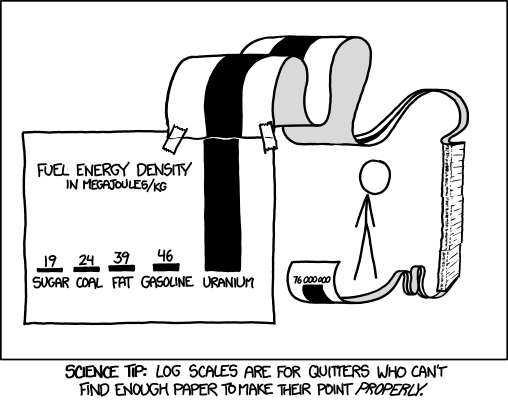
\includegraphics[scale=0.8]{comics/log_scale}
\end{center}

%%%%%%%%%%%%%%%%%%%%%%%%%%%%%%%%%%%%%%%%%%%%%%%%%%%%%%%%%%%%%%%%%%%%%%%%%%%5

\newpage
\section{Der Bachelor Bioinformatik – oder: Wo bin ich hier gelandet?}
\spaltenanfang
Nun seid ihr den ersten Schritt gegangen, und habt euch für den Bachelor Bioinformatik Studiengang an der Johann Wolfgang Goethe Universität eingeschrieben. Damit ihr euch nach den ersten zaghaften Blicken in der Bachelor Ordnung nicht wieder ausschreibt, werde ich versuchen, euch diesen Ordnungswulst zusammengefasst und verständlich wiederzugeben. Es sei allerdings angemerkt, dass Änderungen in der Ordnung noch gemacht werden könnten, die euch betreffen können. Zunächst einmal gilt für euren Bachelor Studiengang, wie für alle Anderen auch, dass er modular aufgebaut ist, und in 6 Semestern mit der Bachelorarbeit zum Ziel führt. Ein Modul umfasst im Allgemeinen eine oder mehrere Lehrveranstaltungen. Es kann außerdem sein, dass zur Anmeldung einer Modulabschlussprüfung bestimmte Auflagen (z.B. der Abschluss eines anderen Moduls, oder der Nachweis einer Studienleistung) erfüllt werden müssen. Weil all dieses noch viel zu trivial ist, kommt noch hinzu, dass Prüfungen von Informatikveranstaltungen nach der Informatik-Prüfungsordnung, und Prüfungen von Bioveranstaltungen von der Biologie-Prüfungsordnung geregelt sind.

Zu der Prüfungsordnung der Informatik zählen: Programmierung 1 (Studienleistung), Programmierung 2 (Studienleistung), Modulabschlussprüfung Programmierung (Thematisch: Programmierung 1 \& 2), Grundlagen der Programmierung für Bioinformatiker Praktikum, Algorithmentheorie, Datenstrukturen, Algorithmen und Modelle der Bioinformatik, Diskrete Modellierung, Analysis und lineare Algebra, Mathe 2 - alternativ Stochastik und Numerik.

Für diese aufgezählten Module gilt: Ihr habt 3 Versuche, wobei der letzte Versuch mündlich sein sollte. Solltet ihr hiernach durchfallen, seit ihr durch den Bachelor Bioinformatik final durchgefallen und dürft in ganz Deutschland keinen Bioinformatik oder Bioinformatik-nahen Studiengang an einer deutschen Hochschule mehr studieren. Es empfiehlt sich also, sich nur dann anzumelden, wenn man auch der Meinung ist, man könne die Prüfung auch bestehen. Eine Ausnahme bilden jedoch Numerik, Mathe 2 und Stochastik. Solltet ihr z.B. in Numerik final durchfallen, und in Stochastik noch nicht eure finale Prüfung hinter euch haben, so seit ihr nicht durch den Bachelor in Bioinformatik durchgefallen, ihr habt jedoch keine Möglichkeit mehr euch in Numerik prüfen zu lassen, und müsst nun Stochastik oder Mathe 2 bestehen. Das Gleiche gilt natürlich auch umgekehrt. Wenn ihr jedoch durch alle 3 durchfallt, seid ihr durch den Bachelor final durchgefallen. Wenn Ihr durch eine Modulabschlussprüfung durchfallen solltet, habt ihr 14 Monate Zeit diese zu wiederholen. Bei den Modulen: Modulabschlussprüfung in Programmierung, Algorithmentheorie, Datenstrukturen, Modellierung, Analysis und lineare Algebra, Stochastik und Numerik handelt es sich um so genannte „Basismodule“. Die Informatik Prüfungsordnung schreibt vor, dass diese Module jedes Semester angeboten werden müssen. Es heißt jedoch nicht, dass hierfür extra nochmal eine Vorlesung stattfinden muss. Der durchgenommene „Stoff“ kann sich also durchaus auch auf das Semester davor beziehen. Für Studienleistungen gilt: Ihr habt soviel Versuche wie ihr wollt. Es gibt keine Limitierungen.

%\includegraphics[width=\linewidth]{comics/FuturamaComics/Comicsfinal/Bioinfocpbafg1}

Zu der Biologie Prüfungsordnung zählen: Struktur und Funktion der Organismen, Struktur und Funktion der Organismen Praktikum, Organische Chemie, Biochemie, Mikrobiologie und Pflanzenphysiologie, Organische Chemie Praktikum, Zellbiologie, Neurobiologie, Molekularbiologie und Genetik, Spezialisierung I, Strukturelle Bioinformatik, Grundlagen der Bioinformatik, Spezialisierung II.

%\includegraphics[width=\linewidth]{comics/FuturamaComics/Comicsfinal/Bioinfocpbafg2}
%\hspace *{1cm}

Für diese aufgezählten Module gilt: Ihr habt auch 3 Versuche. Der letzte Versuch muss jedoch nicht mündlich sein. Wenn er schriftlich ist, wird die Klausur im Falle einer finalen Prüfung von 2 Prüfenden bewertet. Wenn ihr durch eine Modulabschlussprüfung durchfallt müsst ihr diese Prüfung zum nächsten Prüfungstermin wiederholen.

%\includegraphics[width=\linewidth]{comics/FuturamaComics/Comicsfinal/Bioinfocpbafg3}
%\hspace *{1cm}

 Sollte die Prüfung Zulassung für ein Modul im folgenden Semester sein, wird vom Fachbereich Biowissenschaften eine Wiederholungsmöglichkeit vor Beginn des jeweiligen Semesters angeboten.
%\hspace *{1cm}

Solltet ihr bei einer kumulativen Modulprüfung (z.B. in Mikrobiologie und Pflanzenphysiologie) in einer Teilprüfung durchfallen (z.B. Mikrobiologie), so müsst ihr nur die Teilprüfung wiederholen, durch die ihr durchgefallen seid (in unserem Fall Mikrobiologie). Die Gesamtmodulabschlussnote ergibt sich aus dem addierten Mittelwert beider Teilprüfungen.

Eine Ausnahme bilden: Präsentationstechniken, Teammanagement und Führungskompetenz, Wahlpflichtmodul und Abschlussmodul (die Bachelorarbeit). Präsentationstechniken, Teammanagement und Führungskompetenz und das Abschlussmodul können entweder im Bereich der Informatik oder im Bereich der Biologie absolviert werden. Bei dem Wahlpflichtmodul habt ihr sogar noch eine größere Auswahl. Hier könnt ihr frei aus den Veranstaltungen von Biowissenschaften, Informatik und Mathematik, Biochemie, Pharmazie und Chemie oder Physik wählen. Solltet ihr nur ein Fach wählen, müsst ihr 9 CP erbringen. Ihr könnt auch 2 Fächer wählen, jedoch müsst ihr dann jeweils mindestens 6 CP erbringen. Wenn ihr in eurem Wahlpflichtmodul eine Prüfung ablegt, und darauf eine Note bekommt, fließt diese nicht in die Notenberechnung eures Bachelor Zeugnisses ein, ihr könnt jedoch auf Antrag beim Prüfungsausschuss Bioinformatik die Note mit in die Bachelor Urkunde aufnehmen lassen.
%\hspace *{1cm}

Für Teammanagement und Führungskompetenz gibt es folgendende Möglichkeiten, wie ihr die 4CP bekommen könnt: Tutoriumsleitung (PRG 1 oder 2) oder Strufo (Praktikumsbetreuung), IT-Projektmanagement, Ringvorlesung Informatik + Gesellschaft. 

%\begin{center}
%\includegraphics[width=6.5cm]{comics/FuturamaComics/Comicsfinal/Bioinfocpbafg4}
%\end{center}

Solltet ihr nach 6 Semestern alle Prüfungen erfolgreich absolviert haben , wird euer Abschlussmodul für die Berechnung der Gesamtnote CP mäßig doppelt so hoch gewichtet, wie es angegeben ist. Die anderen Module werden anhand ihrer CP anteilig angerechnet (also CP * Note + CP * Note usw. / Alle Module (in CP), auf die Ihr eine Note gekriegt habt, und die in diese Berechnung mit eingerechnet wurden).

%\includegraphics[width=\linewidth]{comics/FuturamaComics/Comicsfinal/Bioinfocpbafg5}

\begin{flushright} Tim, modified by Stefan \end{flushright}
\spaltenende

\vspace{25mm}
\begin{center}
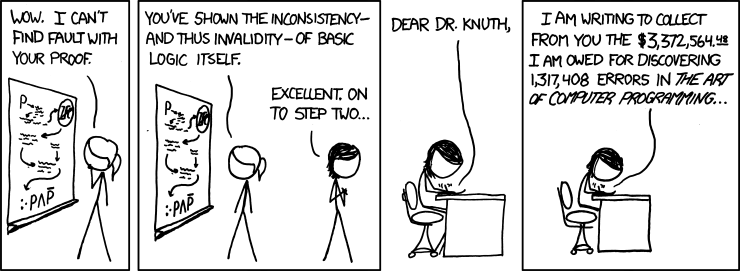
\includegraphics[scale=0.75]{comics/applied_math}
\end{center}

%\newpage

\begin{addmargin}[-5mm]{0cm}

\subsection{Studienverlaufsplan Bioinformatik, falls Stochastik oder Mathe 2 (empfohlen) gewählt wird}

\begin{center}

\begin{tabular}{|c|cc|c|c|c|}
\hline Fach- & Titel der Veranstaltung & Veranst. & Dauer & Dauer & Modul-Nr. \\ 
 semester &  & Form & (SWS) & (CP) &  \\ 
\hline 1. & Struktur + Funktion der Organismen & S,V,Ü,T & 10 & 12 & 1 \\ 
\hline  & Programmierung 1 & V,T & 6 & 9 & 2 \\ 
\hline  & Analysis und lineare Algebra & V,T & 6 & 9 & 3 \\ 
\hline  & \textbf{Summe SWS bzw. CP} &  & \textbf{22} & \textbf{30} &  \\ 
\hline 2. & Programmierung 2 & V,Ü & 5 & 8 & 2 \\ 
\hline  & Grundlagen der Bioinformatik & V,Ü & 4 & 6 & 4 \\ 
\hline  & Angewandte Mathematik & V,Ü & 8V + 4Ü & 9 & 5A oder 5B \\ 
\hline  & Bioorganische Chemie & V,Ü & 5 & 7,5 & 6 \\ 
\hline  & \textbf{Summe SWS}&  & \textbf{20} & \textbf{30,5} &  \\ 
\hline 3. & Grundl. d. Programmierung f. Bioninformatiker & Ü & 4 & 8 & 7 \\ 
\hline  & Biochemie & V & 2 & 3 & 8 \\
        & Tierphysiologie & V & 2 & 3 & 9 \\ 
\hline  & Modellierung & V,Ü & 5 & 7 & 12 \\ 
\hline  & Bioorganische Chemie & Pr, S & 10 & 9,5 & 6 \\ 
\hline  & \textbf{Summe SWS}&  & \textbf{23} & \textbf{30,5} &  \\ 
\hline 4. & Zellbiologie & V & 2 & 3 & 8 \\ 
\hline  & Neurobiologie & V & 2 & 3 & 9 \\ 
\hline  & Molekularbiologie und Genetik & V & 4 & 6 & 11 \\ 
\hline  & Algorithmen und Modelle der Bioinformatik & V,S & 6 & 9 & 13 \\ 
\hline  & Datenstrukturen & V,Ü & 3 & 5 & 14 \\ 
\hline  & Präsentationstechniken & V,S & 3 & 3 & 20 \\
\hline  & \textbf{Summe SWS}&  & \textbf{20} & \textbf{29} &  \\
\hline 5. & Strukturelle Bioninformatik & V,Ü & 4 & 6 & 15 \\ 
          & Spezialisierung 2 & Ü,S & 4 & 6 & 17 \\ 
\hline  & Algorithmentheorie & V,S & 5 & 8 & 18 \\ 
\hline  & Teammanagement und Führungskompetenz & S,TL & 3 & 4 & 19 \\
\hline  & Mikrobiologie und Pflanzenphysiologie & V & 4 & 6 & 10 \\
\hline  & \textbf{Summe SWS}&  & \textbf{20} & \textbf{30} &  \\
\hline 6. & Wahlpflichtmodul &  &  & 9 & 21 \\ 
\hline  & Abschlussmodul & S/T,B &  & 15 & 22 \\ 
\hline  & Spezialisierung 1 & Ü,S & 4 & 6 & 16 \\
\hline  & \textbf{Summe SWS} &  & \textbf{24} & \textbf{30} &  \\ 
\hline  & \textbf{Summe 1. - 6. Sem.} &  &  & \textbf{180} &  \\ 
\hline 
\end{tabular} 

\end{center}

\end{addmargin}

%\newpage

%\newpage

\begin{addmargin}[-5mm]{0cm}

\subsection{Studienverlaufsplan Bioinformatik, falls Numerik gewählt wird}

\begin{center}

\begin{tabular}{|c|cc|c|c|c|}
\hline Fach- & Titel der Veranstaltung & Veranst. & Dauer & Dauer & Modul-Nr. \\ 
 semester &  & Form & (SWS) & (CP) &  \\ 
\hline 1. & Struktur + Funktion der Organismen & S,V,Ü,T & 10 & 12 & 1 \\ 
\hline  & Programmierung 1 & V,T & 6 & 9 & 2 \\ 
\hline  & Analysis und lineare Algebra & V,T & 6 & 9 & 3 \\ 
\hline  & \textbf{Summe SWS bzw. CP} &  & \textbf{22} & \textbf{30} &  \\ 
\hline 2. & Programmierung 2 & V,Ü & 5 & 8 & 2 \\ 
\hline  & Grundlagen der Bioinformatik & V,Ü & 4 & 6 & 4 \\ 
\hline  & Bioorganische Chemie & V,Ü & 5 & 7,5 & 6 \\ 
\hline  & Zellbiologie & V & 2 & 3 & 8 \\ 
\hline  & \textbf{Summe SWS}&  & \textbf{18} & \textbf{26} &  \\ 
\hline 3. & Grundl. d. Programmierung f. Bioninformatiker & Ü & 4 & 8 & 7 \\ 
\hline  & Biochemie & V & 2 & 3 & 8 \\
        & Tierphysiologie & V & 2 & 3 & 9 \\ 
\hline  & Angewandte Mathematik & V,Ü & 8V + 4Ü & 9 & 5A oder 5B \\
\hline  & Modellierung & V,Ü & 5 & 7 & 12 \\ 
\hline  & \textbf{Summe SWS}&  & \textbf{25} & \textbf{30} &  \\
\hline 4. & Neurobiologie & V & 2 & 3 & 9 \\
\hline  & Molekularbiologie und Genetik & V & 4 & 6 & 11 \\ 
\hline  & Algorithmen und Modelle der Bioinformatik & V,S & 6 & 9 & 13 \\ 
\hline  & Datenstrukturen & V,Ü & 3 & 5 & 14 \\ 
        & Bioorganische Chemie & Pr, S & 10 & 8 & 6 \\
\hline  & \textbf{Summe SWS}&  & \textbf{24} & \textbf{31} &  \\
\hline 5. & Strukturelle Bioninformatik & V,Ü & 4 & 6 & 15 \\ 
          & Spezialisierung 2 & Ü,S & 4 & 6 & 17 \\ 
\hline  & Algorithmentheorie & V,S & 5 & 8 & 18 \\ 
\hline  & Teammanagement und Führungskompetenz & S,TL & 3 & 4 & 19 \\
\hline  & Präsentationstechniken & V,S & 3 & 3 & 20 \\
\hline  & Mikrobiologie und Pflanzenphysiologie & V & 4 & 6 & 10 \\
\hline  & \textbf{Summe SWS}&  & \textbf{23} & \textbf{33} &  \\
\hline 6. & Wahlpflichtmodul &  &  & 9 & 21 \\ 
\hline  & Abschlussmodul & S/T,B &  & 15 & 22 \\ 
\hline  & Spezialisierung 1 & Ü,S & 4 & 6 & 16 \\
\hline  & \textbf{Summe SWS} &  & \textbf{24} & \textbf{30} &  \\ 
\hline  & \textbf{Summe 1. - 6. Sem.} &  &  & \textbf{180} &  \\ 
\hline 
\end{tabular} 

\end{center}

\end{addmargin}

%\newpage


%%%%%%%%%%%%%%%%%%%%%%%%%%%%%%%%%%%%%%%%%%%%%%%%%%%%%%%%%%%%%%%%%%%%%%%%%%%5

\section{Apropos Pädagogik: Informatik L3}

\spaltenanfang
\spaltenanfang
Seit dem Wintersemester 1997/98 kann man in Frankfurt Informatik auf Lehramt im L3-Studiengang (Gymnasiales Lehramt) studieren, seit dem Wintersemester 2010/11 zudem auch im L2-Studiengang (Haupt- und Realschullehramt) und im L5-Studiengang (Förderschule)  – mit sehr guten Berufsaussichten, denn viele entschließen sich nicht dazu und viele hören schon bald wieder auf.
Warum eigentlich? So ein Info-Lehramtsstudium ist doch ganz einfach.

Zunächst einmal stellen wir die für das Lehramtsstudium relevanten Ämter vor:

LA - \textit{Die hessische Lehrkräfteakademie}

Die hessische Lehrkräfteakademie (LA) (ehemals: LSA /Landesschulamt, und davor AfL / Amt für Lehrerbildung).
Die LA ist dem Hessischen Kultusministerium direkt untergeordnet und ist verantwortlich für die Ausbildung von Lehrkräften aller Fachrichtungen und Schulformen in ganz Hessen.
Du wirst im Regelfall mit der LA direkt nur max. dreimal zu tun haben: Bei deinem „Orientierungspraktikum“ und bei deinem „Betriebspraktikum“ und deinem 1. Staatsexamen.
Kontakt mit der LA kannst du am besten aufnehmen, indem du an den zuständigen Sachbearbeiter eine E-Mail schickst oder anrufst.


SPS-Büro \textit{Büro für Schulpraktische Studien}

Das SPS-Büro der ABL (Akademie für Bildungsforschung und Lehrerbildung) übernimmt innerhalb der Goethe-Universität die Koordination der Schulpraktischen Studien (SPS), auch hierzu später mehr. Du findest das SPS-Büro momentan im Juridicum auf dem Campus Bockenheim im 10. OG.
Du meldest dich beim SPS-Büro für die Schulpraktischen Studien an und im Gegensatz zu allen anderen Ämtern an der Universität muss dem SPS-Büro eine Änderung deines Studiums explizit (schriftlich) mitgeteilt werden (z.B.: bei einem Fachwechsel). Die Anmeldefristen für die SPS findest du auf der Homepage des SPS-Büros (www.abl.uni-frankfurt.de/40729270/Schulpraktische-Studien ). Diese Fristen sind absolut verbindlich und es gibt keinen Spielraum – also hier besonders genau sein!


ZPL – \textit{Zentrales Prüfungsamt für Lehramtsstudiengänge}
Das ZPL befindet sich momentan am Campus Bockenheim im 10 Stock Juridicum. Es ist dafür verantwortlich, die von dir abgelegten Prüfungen (abgeschlossene Module) zu registrieren und die Zwischenprüfung, sowie die Meldung zur ersten Staatsprüfung zu verwalten.
Zu Beginn deines Studiums meldest du dich zur Zwischenprüfung beim ZPL an (Informationen bekommst du entweder auf der Homepage des ZPL, oder bei einer Einführungsveranstaltung). Du legst die Zwischenprüfung automatisch ab, wenn du in vollständig abgeschlossenen Modulen insgesamt 90 CP beim ZPL in Form von kopierten (!) Modulscheinen eingereicht hast - bei L2 brauchst du sogar nur 60 CP.
Die Zwischenprüfung kannst du ablegen, sobald du die benötigten CP gesammelt hast (hierbei gibt es genauere Auflagen, die du der Studienordnung entnehmen kannst), sie sollte allerdings spätestens zwei Semester vor der Meldung zur Ersten Staatsprüfung eingereicht werden, damit eventuelle formale Probleme behoben werden können.
Die Bescheinigung über ein ordnungsgemäßes Studium am Ende bekommst du übrigends genauso. Du reichst alle deine kopierten (!) Modulscheinen ein. Auch das solltest du mindestens ein Semester vor der Meldung zur Ersten Staatsprüfung machen.\\

Neben diesen Ämtern möchten wir dir einige Informationen zu einigen wichtigen Begriffen und Punkten im Lehramtsstudium geben.

\paragraph{Die Schulpraktischen Studien (SPS)}
Die SPS sind der praktische Teil der universitären Lehramtsbildung. Du wirst im Studiengang L2 bzw. L5 in deinem Studium zwei SPS-Veranstaltungen absolvieren, eine bildungswissenschaftliche und eine fachwissenschaftliche. Die SPS setzen sich in dem Fall aus einem Vorbereitungsseminar in einem Semester, einem 5- wöchigen Schulpraktikum in den Semesterferien und einer Nachbereitungsveranstaltung im folgenden Semester zusammen.
L3 Studierende fallen in die Praxissemesterregelung. Ihr habt nur ein Praktikum das über ein Semester geht. Mehr erfahrt ihr unter:http://www.abl.uni-frankfurt.de/51930903/Praxissemester-L3

\paragraph{Modulscheine}
Im Gegensatz zu den meisten anderen Studiengängen ist das Lehramtsstudium noch nicht vollständig digitalisiert. Du kannst dir auf der Seite des ZPL sog. „Modulscheine“ ausdrucken, in welche die Dozenten die Prüfungsnoten eintragen müssen.
In der Regel ist es so, dass zu einem Modul mehrere Veranstaltungen gehören, in diesem Fall ist es empfehlenswert in der zweiten Veranstaltung nur eine Kopie des bereits zum Teil ausgefüllten Scheins abzugeben, denn ein Verlust ist für dich mit erheblicher Arbeit verbunden.

\paragraph{Die fachspezifischen Anhänge und die Studienordnung}
Die Studienordnung für Lehramtsstudiengänge setzt sich aus der
"Studienordnung" und den "fachspezifischen Anhängen" zusammen. Die Studienordnung regelt generelle Formalia, wie zum Beispiel den Umfang des Studiums, die benötigten CP und die Abläufe der Ersten Staatsprüfung und der Zwischenprüfung.
Die fachspezifischen Anhänge hingegen beschränken sich auf ein Fach (z.B.: L3 Informatik) und beinhalten eine Übersicht über die zu belegenden Module.
Sowohl die Studienordnung, als auch die fachspezifischen Anhänge finden sich auf der Homepage der ABL und sind leicht über eine Suchmaschine unter dem Stichwort "fachspezifische Anhänge Uni Frankfurt" zu finden.
\textbf{Zu Beginn des Studiums empfiehlt sich auf jeden Fall eine Lektüre der Studienordnung sowie der fachspezifischen Anhänge.}
Innerhalb der fachspezifischen Anhänge findest du einen Studienverlaufsplan, also einen exemplarischen Plan, in welcher Reihenfolge und in welchem Semester du welche Veranstaltungen belegen kannst. Die Vorgaben sind allerdings nicht verpflichtend, manchmal muss aber auf die Reihenfolge geachtet werden.

\paragraph{Orientierungspraktikum (OP) (betrifft nicht L3-Erstis)}
Das OP muss durch das LA bestätigt worden sein, bevor du dich für die ersten SPS anmelden kannst. Es muss in einer pädagogischen Institution stattfinden und 4 Wochen (120 Stunden) dauern. Auf der Homepage des LA befindet sich ein Vordruck für einen Praktikumsbericht, der ausgefüllt werden muss. Auf der letzten Seite des Berichts ist ein Formular das von dir und vom Betrieb auszufüllen ist, zudem muss vom Betrieb eine (informelle) Bestätigung ausgestellt werden.
Für das OP können Tätigkeiten aus FSJ oder ähnlichem anerkannt werden, in diesem Fall muss nur eine Bescheinigung des Betriebs beiliegen sowie die letzte Seite ausgefüllt werden. Der Bericht entfällt in diesem Fall.
Zu beachten: Ihr könnt euch nichts anrechnen lassen was ihr in eurer Schulzeit gemacht habt.

\paragraph{Betriebspraktikum (BP) (betrifft nicht L3-Erstis)}
Das Betriebspraktikum umfasst 8 Wochen bei "branchenüblicher Arbeitszeit" (in Ordnung sind auch zwei mal 4 Wochen, auch in unterschiedlichen Betrieben). Es muss in einem Betrieb stattfinden, der nichts mit (pädagogisch-) sozialen Tätigkeiten zu tun hat. Auch hierzu findest du auf der Homepage des LA einen Vordruck für einen Praktikumsbericht. Es wird eine Bestätigung des Betriebs benötigt.
Als Betriebspraktikum können Nebenjobs in nicht-pädagogischen Betrieben anerkannt werden, die über einen längeren Zeitpunkt gemacht wurden. In diesem Fall benötigst du eine Bestätigung des Betriebs und musst den Bericht dennoch schreiben!
Das Betriebspraktikum muss vor der Meldung zur Ersten Staatsprüfung eingereicht werden.
\spaltenende

\spaltenende

\definecolor{hellgrau}{gray}{0.8}



\begin{center}
\begin{tabular}{lllcc}

       \textbf{Sem.} & \textbf{Lehrform} & \textbf{Lehrveranst./Modul} & \textbf{CP} & \textbf{SWS} \\ 
\hline 1 &  V+Ü  & PRG-1 aus L3-CS-PRG &  9  &  6  \\
       1 &  V+Ü  & EDI-1 aus L3-CS-EDI &  3  &  2  \\
\hline 2 &  V+Ü  & PRG-2 aus L3-CS-PRG &  8  &  5  \\
       2 &  V+Ü  & EDI-2 aus L3-CS-EDI &  3  &  2  \\
\hline 3 &  V+Ü  & L3-CS-MOD           &  7  &  5  \\
       3 &  S/PR & Didaktik            &  3  &  2  \\
\hline 4 &  V+Ü  & L3-CS-HWR           &  8  &  5  \\
       4 &  S/PR & Didaktik            &  3  &  2  \\

\rowcolor{hellgrau}

\hline   &       & \textbf{Zwischenprüfung}     &     &    \\
\hline 5 &  V+Ü  & L3-CS-M             &  9  &  6  \\
       5 &  S/PR & Didaktik            &  3  &  2  \\
\hline 6 &  S    & L3-CS-S             &  4  &  2  \\
       6 &  V+Ü  & L3-CS-DS            &  5  &  3  \\
       6 &  S/PR & Didaktik            &  3  &  2  \\
\hline 7 &  PR   &  PRG-P R            &  6  &  3  \\
       7 & S/PR  & Didaktik            &  3  &  2  \\
\hline 7/8 & V+Ü/S &  L3-CS-GL         &  8  &  5  \\
       8 & S/PR  & Didaktik            &  3  &  2  \\

\rowcolor{hellgrau}

\hline   &       & \textbf{Staatsexamen}        &     &     \\
\hline   &       &                     & \textbf{88}  &  \textbf{56} \\
         &       & davon Didaktik:     & 24  &  16 \\

\end{tabular}
\end{center}

%%%%%%%%%%%%%%%%%%%%%%%%%%%%%%%%%%%%%%%%%%%%%%%%%%%%%%%%%%%%%%%%%%%%%%%%%%%

\newpage
\section{Veranstaltungs- und Prüfungsformen}

\spaltenanfang
Im folgenden werden wir verschiedene Veranstaltungs- und Prüfungsformen, die dir während deines Studiums über den Weg laufen können, kurz vorstellen, damit du dich darauf einstellen kannst, was alles auf dich zukommen kann. Die unten aufgezählten weiteren Kriterien können euch bei den Modulprüfungen begegnen. In jedem Fall müssen die genauen Kriterien für die zu erbringenden Leistungen spätestens in der ersten Veranstaltungswoche von dem Professor bekanntgeben werden, der die Veranstaltung hält.


\paragraph{Protokolle} In den Praktika musst du meistens wöchentlich eine oder ein paar Aufgaben lösen und diese sehr ordentlich und ausführlich protokollieren. Nur wer alle (oder fast alle – je nachdem) Versuchsprotokolle mit einem „ok“ gekennzeichnet bekommen hat, bekommt einen Praktikumsschein. Es kann aber auch möglich sein, dass zusätzlich noch mehr verlangt wird: Das Bestehen einer Klausur, das Teilnehmen an einem Seminar. Der Phantasie sind da kaum Grenzen gesetzt.


\paragraph{Hausarbeit} Hausarbeiten sind in der Informatik unüblich, in anderen Fächern wie zum Beispiel Pädagogik oder Politologie in Seminaren aber aufgrund der hohen Teilnehmerzahlen durchaus gebräuchlich. Eine Hausarbeit kannst du dir als einen mittelgroßen Aufsatz vorstellen, der nicht mit einem mündlichen Vortrag oder Referat verbunden ist. Und was „mittelgroß“ bedeutet, hängt unter anderem davon ab, wie lang oder wie kurz du ein bestimmtes Thema bearbeiten kannst. Im Zweifelsfall wird dir aber dein Veranstalter einen Tipp geben.


\paragraph{Referat} Referate sind in der Informatik ebenfalls unüblich, hier musst du in der Regel einen kurzen Vortrag über ein bestimmtes Thema halten, manchmal ist zusätzlich eine schriftliche Zusammenfassung zu leisten.


\paragraph{Seminar} Hier ist in der Regel eine schriftliche Ausarbeitung und ein Vortrag (mit anschließender Diskussion) zu einem bestimmten Thema zu leisten. Der Aufwand sollte nicht unterschätzt werden, da je nach Thema einiges an Literatur recherchiert und durchgearbeitet werden muss.

\paragraph{Vorlesung} Hier trägt der Veranstalter zu einem bestimmten Thema vor, dass dann auch in Übungen, falls angeboten, vertieft wird. Du kannst dir Vorlesungen als Frontalunterricht vorstellen, bei dem du zuhören darfst und solltest. Wenn du Glück hast, darfst du sogar ab und zu eine Frage stellen. Ganz engagierte Dozenten stellen sogar ab und zu eine Frage an die Hörer, um sicherzustellen, dass sie ihm auch gedanklich folgen. Vorlesungen an der Universität verlaufen aber oft sehr viel schneller als die Kurse in der Schule. Das heißt: \textbf{Passt du heute nicht auf, weißt du morgen schon nicht mehr, worum es überhaupt geht,} und aufzupassen fällt dir immer schwerer, und übermorgen gehst du vor lauter Frust schon gar nicht mehr hin. Die Übungszettel sind eine Möglichkeit für dich, sich mit dem Stoff der Vorlesung nochmal auseinanderzusetzen. Immerhin bist du nicht gezwungen, die Aufgaben allein zu lösen, sondern du darfst dich mit deiner Lerngruppe an die Zettel setzen, und mit mehreren Leuten hat man ja oft auch mehr Ideen. 


\paragraph{Mündliche Prüfung, „Fachgespräch“} Mündliche Fachgespräche werden oft in Vorlesungen Angeboten, wenn zu erwarten ist, dass sich nicht allzu viele Studis prüfen lassen werden. Ein 
solches Gespräch soll 20 bis 40 Minuten dauern. Am besten, du schaust dir vorher mal Prüfungsprotokolle an (beispielsweise auf der Homepage der Fachschaft angeboten), damit du einen Eindruck vom Prüfungsstil und den Lieblingsfragen des Prüfers bekommst.


\paragraph{Klausur} Eine Klausur ist in vielen Basismodulen vorgesehen. Sie dauert zwei bis vier Stunden, zum Bestehen musst du einen bestimmten Anteil der möglichen Punkte auch wirklich erreichen. Meistens liegt dieser Anteil so grob bei 50 \%, es kann je nach Fach und Schwierigkeit des Stoffs aber auch weniger sein!


\paragraph{Übungen} Jede Woche bekommst du einen Zettel mit Aufgaben, die du bis zur folgenden Woche lösen sollst. In den  „Tutorien“ oder „Übungen“ werden sie dann besprochen (dazu weiter unten noch mehr). Übungen sind etwas anders als Hausaufgaben. Einerseits solltest du sie zu Hause lösen. Andererseits bekommst du aber auch keine 6 eingetragen, wenn du sie nicht machst. Du musst dir noch nicht einmal eine gute Ausrede einfallen lassen.

Oft werden die letzten beiden Kriterien, Klausur und Übungen, kombiniert: Es gibt Übungsaufgaben, und die Punkte, die du damit erreichst, werden schon für die Klausur angerechnet; oder sie dienen dir nur zu deiner Vorbereitung auf die Klausur.


\paragraph{Tutoriumsleitung} Im Bachelor-Studiengang ist es möglich, durch das Leiten eines Tutoriums das Ergänzungsmodul zu komplettieren. Dadurch hast du nicht nur die Möglichkeit, das Institut für Informatik direkt zu unterstützen, sondern kannst außerdem noch wertvolle Erfahrungen im Bereich der Soft Skills sammeln.


\paragraph{Tutorien} Und wie ist das mit den Tutorien? Einmal in der Woche findet eine Veranstaltung bei eurem Tutor statt. Das ist auch ein Studi, der mit seinem Studium schon weiter ist und sich jetzt bereit erklärt hat, euch ein wenig beim Studieren zu helfen. Während eines solchen Tutoriums werdet ihr die Übungsaufgaben besprechen; meistens wird einer von euch eine Aufgabe vorrechnen. Das hat nichts damit zu tun, euch „vorführen“ zu wollen. Es sind aber zwei verschiedene Dinge, eine Lösung auf einen Zettel zu malen und eine Lösung anderen laut und mündlich, mit Hilfe einer Tafel, zu erklären. Die Möglichkeit, das zu üben, solltet ihr euch nicht entgehen lassen; ihr profitiert davon nicht nur für Seminarvorträge! Auch wenn ihr von eurem Tutor Punkte auf eure Lösungsversuche bekommt (oder viel zu oft nicht bekommt), ist es für euch keine Schande zuzugeben, dass ihr etwas nicht verstanden habt und euren Tutor danach zu fragen. Dafür sind Tutorien da!

Es ist wohl möglich, existierende Lösungen abzuschreiben und sich in den Tutorien wie eine Maus zu verkriechen und bloß nicht aufzufallen. Es haben auch schon Leute auf diese Weise einen Übungsschein (ohne Klausur) erhalten. Ihr wisst schon, gelernt will der Stoff trotzdem werden, denn in der mündlichen Prüfung gibt es kein Abschreiben und Verstecken.


Oft aber verlaufen Tutorien ganz anders. Der Tutor schreibt an und wirbelt herum, reißt sich ein Bein aus und redet sich ’nen Wolf, und alle Teilnehmer sitzen gelangweilt im Seminarraum, gucken an die Decke und bohren in der Nase. Was glaubt ihr, könnt ihr in einem solchen Tutorium lernen? Na? Wie sinnvoll und interessant und hilfreich ein Tutorium ist, ist zu einem großen Teil davon abhängig, wie die Teilnehmer es gestalten. Macht was draus!

\begin{flushright}Oliver und Sebastian\end{flushright}
\spaltenende

\vspace{1cm}

\begin{center}
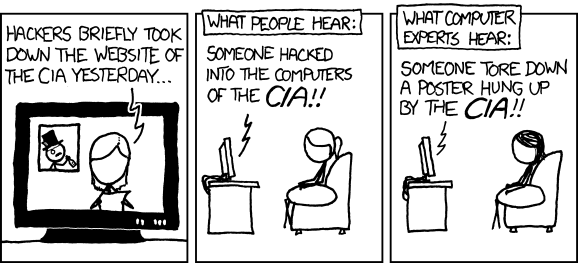
\includegraphics[scale=0.8]{comics/cia}
\end{center}

%%%%%%%%%%%%%%%%%%%%%%%%%%%%%%%%%%%%%%%%%%%%%%%%%%%%%%%%%%%%%%%%%%%%%%%%%%%

\newpage
\section{Goethe-Card}

%\spaltenanfang
\begin{wrapfigure}[8]{r}{0.48\textwidth}
     \vspace{-5mm}
  \begin{center}
     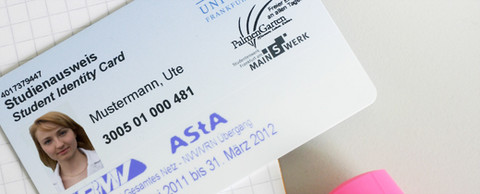
\includegraphics[scale=0.5]{bilder/goethecard}
  \end{center}
\end{wrapfigure}

Nach der erfolgreichen Immatrikulation an unserer Universität bekommst du im Studien-Service-Center eine schicke Chipkarte mit deinem Foto und einigen bildhaften Logos und Beschriftungen drauf. Möglicherweise erfährst du auch gleich, dass sie \emph{Goethe-Card} heißt und als Studienausweis dient. Warum braucht man überhaupt so etwas, wenn man bereits einen ordinären Ausweis hat?

Der wichtigste Grund ist die Tatsache, dass man damit sofort feststellen kann, ob du zum aktuellen Zeitpunkt an der Goethe-Universität studierst: In diesem Fall wurde das blau aufgetragene Gültigkeitsdatum unten zu diesem Zeitpunkt noch nicht überschritten. 

Falls du jetzt ein Blick auf deinen Studienausweis wirfst, wirst du bemerken, dass dort als Enddatum der letzte Tag des laufenden Semesters steht. Daher wirst du, solange du bei uns bleibst, einmal alle 6 Monate diesen Eintrag updaten müssen. Das geht über einen der mehreren extra dafür erstellten und überall auf dem Uni-Gebiet platzierten Automaten, die oft auch \emph{Validierer} genannt werden. Sollte man sein Studium absolviert oder abgebrochen haben, wird der Validierer das Enddatum der Gültigkeit nicht ändern.

Auf der Goethe-Card sind außerdem dein Foto, dein Name und auch deine persönliche Identifikationsnummer (\emph{Matrikelnummer}) in der Universität aufgeschrieben\footnote{Deine Matrikelnummer ist 7-stellig und entspricht den letzten 7 Ziffern der 12\hbox{-}stelligen Zahl auf dem Goethe-Card.}. Diese Angaben helfen nicht nur den Profs, dich eindeutig zu identifizieren, sondern auch dir, deine während der Prüfung vergessene Matrikelnummer schnell zu finden.

Aber das ist noch nicht alles, was du mit der Goethe-Card machen kannst:

\begin{itemize}
	\item Du kannst darauf mittels spezieller Geldautomaten-ähnlichen Geräten darauf \textbf{Geld aufladen}, um damit in der Mensa für das Essen oder auch in der Uni-Bibliothek für die Verwendung des Kopierers zu bezahlen
	\item Du kannst sie als einen \textbf{digitalen Schlüssel} für die super modernen Schließfächer am Campus Westend verwenden
	\item Du kannst damit \textbf{kostenlos} den \textbf{Palmengarten} besuchen
	\item Du kannst damit\textbf{ Bücher in der Uni-Bibliothek ausleihen}
\end{itemize}

Und - last but not least - du kannst damit \textbf{kostenlos} in allen öffentlichen Verkehrsmitteln außer ICE, IC und EC in Hessen fahren! Vor dem 01.03.2013 war das NVV-Gebiet leider nicht mit dabei, daher solltest du deine Goethe-Card unbedingt updaten, wenn du diese vor diesem Tag erhalten hast und kein Logo von NVV neben dem Logo von RMV siehst.

Allerdings pass auf: Außerhalb von Hessen funktioniert das nicht mehr! Auf der nächsten Seite findest du eine Karte mit dem skizzierten Geltungsbereich des Semestertickets.

Ausserdem: Der Verlust der Goethe-Card kann recht schmerzlich sein - z.Z. liegt die Gebühr bei Verlust und darauf folgende Neubeantragung (Campus Westend) bei 50 Euro.

Weitere Informationen zur Goethe-Card kannst du bei Interesse hier finden:\\
\url{http://www.rz.uni-frankfurt.de/44160530/Goethe-Card}
\begin{flushright}Pavel, korrigiert von Sabrina \end{flushright}
%\spaltenende

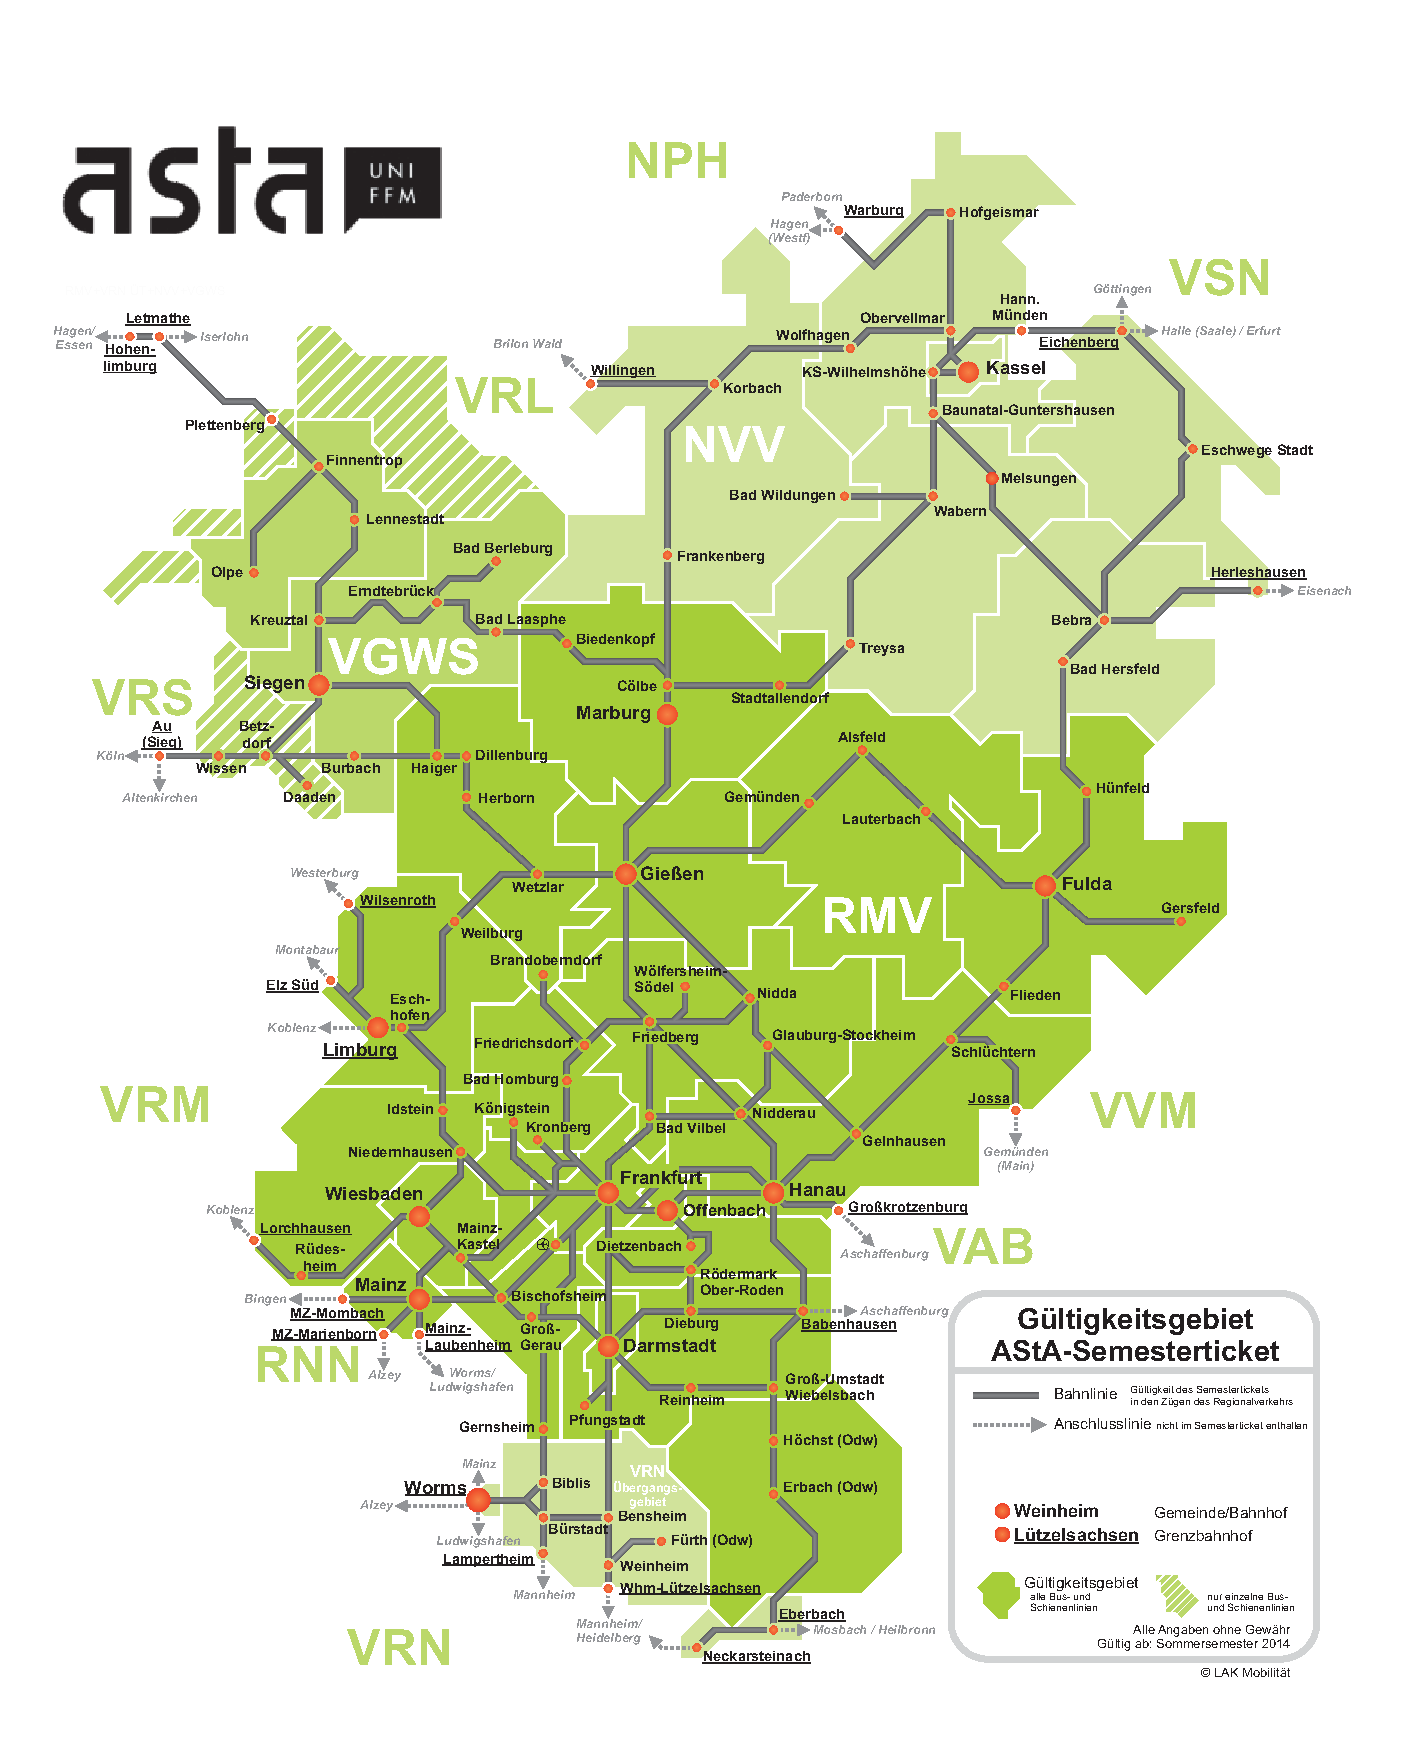
\includepdf{bitmaps/semesterticketgueltigkeitsbereich2014}
%\begin{center}
%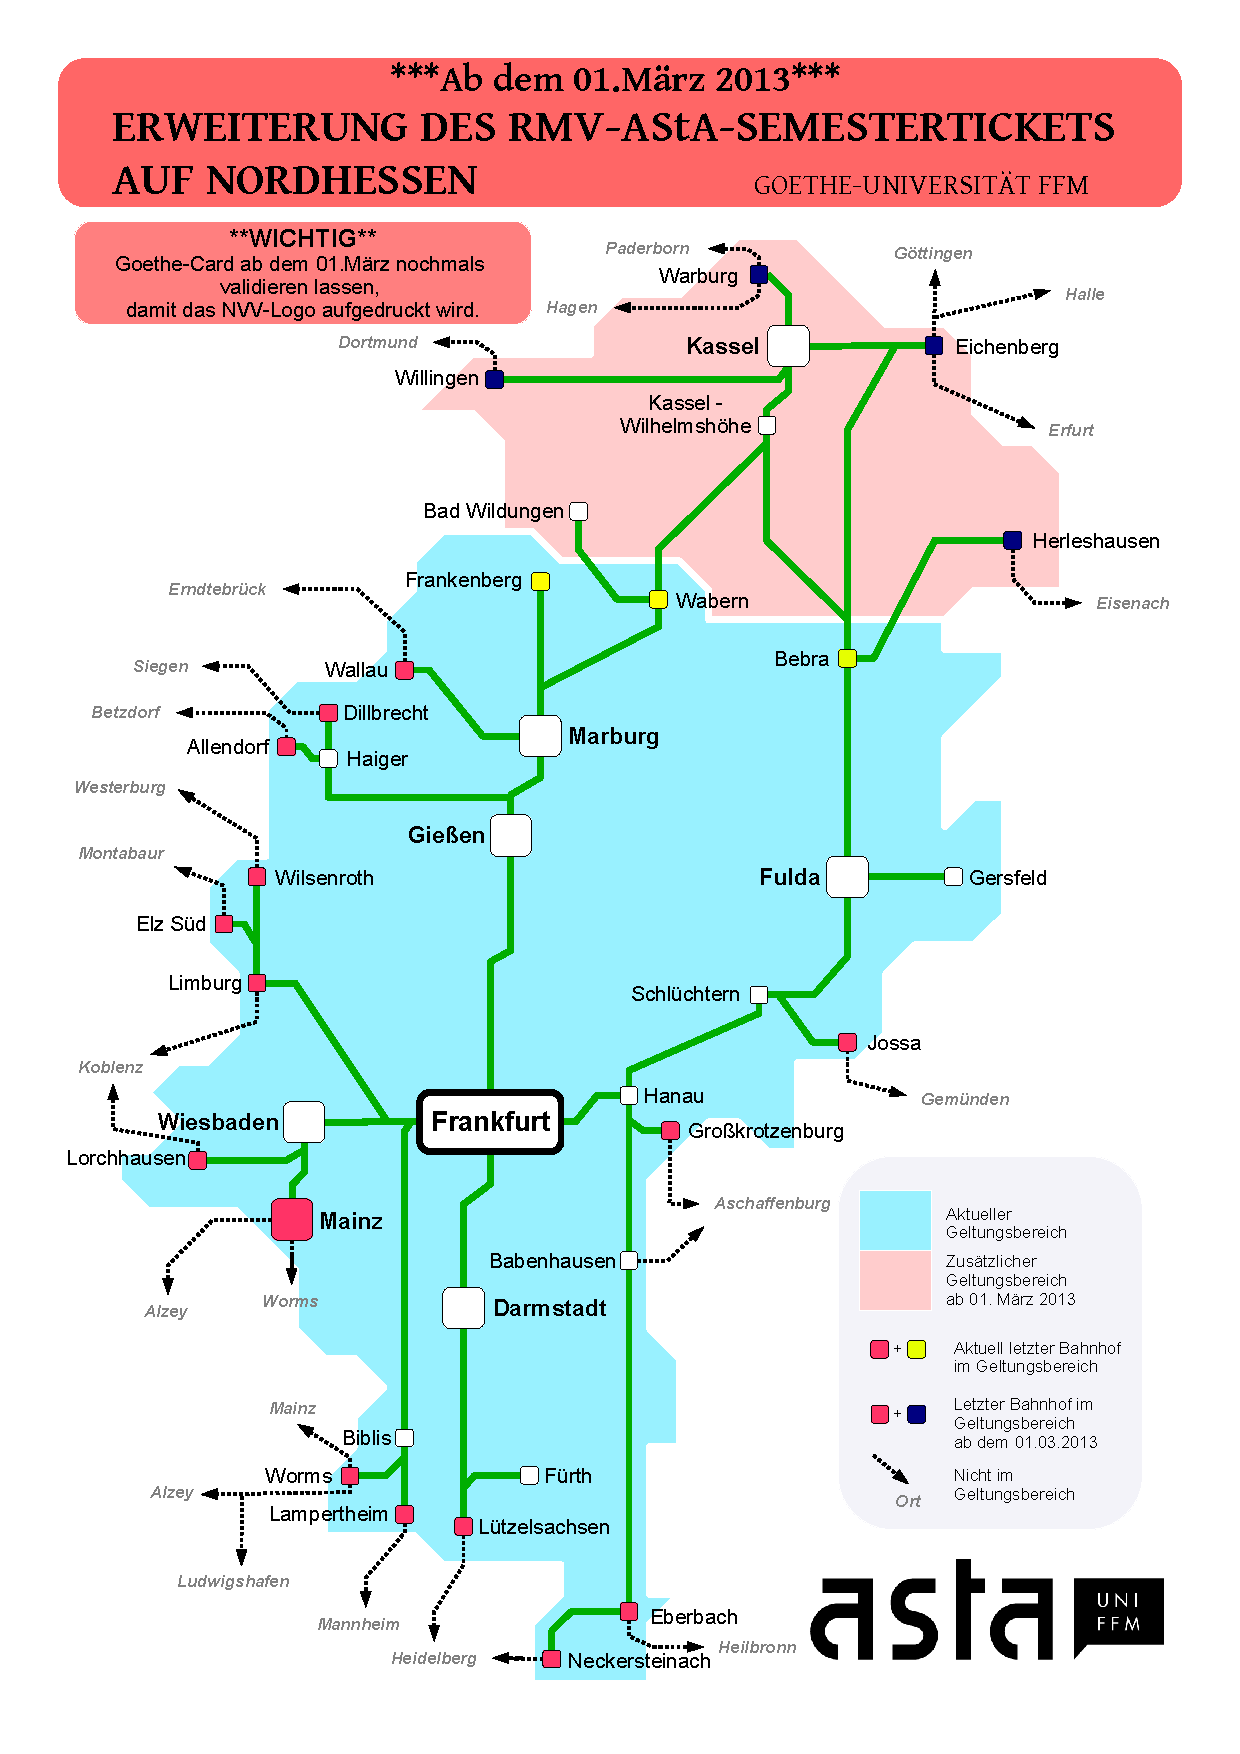
\includegraphics[scale=1.0]{tabellen/geltungsbereichabsose2013-asta-version-bildfuerhp}
%\end{center}

%%%%%%%%%%%%%%%%%%%%%%%%%%%%%%%%%%%%%%%%%%%%%%%%%%%%%%%%%%%%%%%%%%%%%%%%%%%

\newpage
\section{Peer Mentoring}

\spaltenanfang
\spaltenanfang
Die Erste Regel des Mentoring ist: alle reden über das Mentoring.
Die Zweite Regel des Mentoring ist: ALLE reden ÜBER das Mentoring.
Die Mittlere Regel des Mentoring ist: wenn jemand schlappmacht... naja, dafür sind wir ja da.
Die Vorletze Regel des Mentoring ist: was im Mentoring gesagt wird, bleibt im Mentoring.
Die Letzte Regel des Mentoring ist: wer neu ist muss rein... ne, wirklich. Ist so.

Die Veranstaltung ''STO (STudienOrientierung) - Einführung in das Studium'', im Volkmund ''Das Mentoring'' genannt, ist Teil des sogenannten Ergänzungsmoduls und ihr \emph{müsst} es besuchen, um euren Bachelor Informatik zu bekommen. Ihr verdient hier sage und schreibe ganze \emph{2 CP}, wenn ihr es jetzt und sofort, also im \textbf{ersten Semester} besucht. \emph{Nur 1 CP} hingegen bekommt ihr, wenn ihr dieses Modul in einem späteren Semester abschließt. Überdies sind die Informationen, die ihr dort bekommt, vor allem in den ersten Semestern relevant. Weil STO überhaupt nicht anstrengend ist, könnt ihr es problemlos neben all den anderen Dingen besuchen, die euch möglicherweise viel Zeit und viele Nerven rauben. Außerdem soll euch genau jene Veranstaltung gerade ein kleines bisschen ein Führer durch den Informatik-Uni-Dschungel sein und dabei helfen, dass ihr vielleicht nicht ganz so viel Zeit und Nerven verliert. 

Was?: STO besteht aus einer Vorlesung und einem Kleingruppentreffen (mit 5 Terminen, über das Semester verteilt), genannt Peer-Mentoring. 

Warum?: Es geht hier darum, dass ihr den Einstieg in euer Studium besser findet, denn aller Anfang ist schwer. Im Laufe eures Studiums werdet ihr merken, dass an der Uni zu studieren auch bedeutet, eigenverantwortlich zu arbeiten: Ihr habt kaum Anwesenheitspflichten, müsst euch euren Stundenplan (zumindest später) selbst zusammenstellen und könnt selbst entscheiden, wie viel Übungs- und Lernaufwand ihr betreiben wollt. 
Ihr habt also viele Freiheiten, solltet dabei aber nicht den Kopf verlieren. Der Kopf bleibt auf dem Hals und ihr behaltet von dort aus den Überblick, wenn ihr möglichst viel über euer Studium wisst, denn dann könnt ihr anständig planen.
Die STO-Vorlesung und das Mentoring (Kleingruppentreffen) sollen euch dabei helfen, dieses Studienwissen zu erlangen. Alle Fragen die ihr rund um das (Informatik-)Studium habt, sollt ihr im Mentoring stellen. Ihr könnt dort außerdem thematisieren (oder euren Mentor direkt persönlich ansprechen), wenn sich euer Leben durch das Studium verändert hat und ihr an dieser Stelle Ratschläge braucht. Das bedeutet natürlich, dass alles was im Mentoring gesagt wird, auch im Mentoring bleiben soll.

Wie?: Ihr besucht die erste STO-Vorlesung am \textbf{16.04.2015} (Vorlesungsverzeichnis) und erfahrt dort, wie ihr euch in die Mentorings einschreibt.
\spaltenende

\spaltenende


\begin{center}
	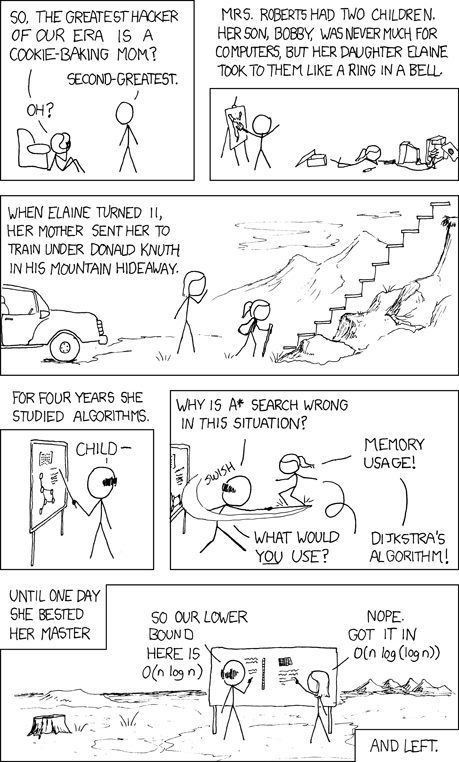
\includegraphics[scale=0.88]{comics/1337_part_2}
\end{center}

%%%%%%%%%%%%%%%%%%%%%%%%%%%%%%%%%%%%%%%%%%%%%%%%%%%%%%%%%%%%%%%%%%%%%%%%%%%

%\newpage
%\section{Von Studien- und Prüfungsleistungen}
%\label{studienleistungen}

%\spaltenanfang
%Damit du dein Studium auch erfolgreich beenden kannst, musst du irgendwann auch Prüfungen ablegen.
Du wirst warscheinlich schon im ersten Semester deine ersten Klausuren schreiben wollen, um die Veranstaltungen abzuschließen.
Im Bachelorstudiengang wird zwischen zwei verschiedenen Prüfungen unterschieden: \emph{Prüfungsleistungen} und \emph{Studienleistungen}.
Die erste Frage, die sich stellt ist, was denn der Unterschied zwischen beidem ist.
Nun, im ersten Semester wirst du den als einzigen Unterschied spüren, dass du für die Studienleistungen kein Formular ausfüllen musst während du für Prüfungsleistungen ins Prüfungsamt rennen musst.
Im zweiten Semester wirst du merken, dass du für \emph{Grundlagen der Programmierung} und die beiden Technikveranstaltungen noch einmal eine mündliche Prüfung ablegen musst.
Warum das?

Nun, wenn du dir die Modulübersicht ansiehst, wirst du merken, dass \emph{PRG-1} und \emph{PRG-2} zusammen ein Modul bilden.
Das gleiche gilt für die Paare \emph{EDGI} und \emph{HWR} sowie \emph{GL-1} und \emph{GL-2}.
In allen Veranstaltungen außer diesen sechs ist die Prüfung am Ende des Semesters eine \emph{Prüfungsleistung}, die auch \emph{Modulabschlussprüfung} genannt wird.
Dieser Name macht deutlicher, was gemeint ist:
Die Prüfung schließt das Modul komplett ab und die Note wird später in deine Bachelornote verrechnet.
In den sechs oben genannten Veranstaltungen ist die Prüfung nicht eine Modulabschlussprüfung, da das Modul ja aus beiden Veranstaltungen besteht.
Mit der Klausur hier zeigst du lediglich, dass du den Stoff aus dem Semester verstanden hast.
Um diese ``Doppelmodule'' abzuschließen musst du eine zusätzliche mündliche Prüfung machen.
Diese mündliche Prüfung ist dann die Modulabschlussprüfung, deren Note in deinen Bachelor zählt.
Um zu der mündlichen Prüfung zugelassen zu sein, musst du aber mindestens eine der Klausuren bestanden haben.

Nun habe ich sehr viele verwirrende Dinge erzählt, die du erst einmal verdauen musst, aber \textbf{Don't Panic}: so schwer, wie es klingt ist das nicht.
Spielen wir mal eine Prüfungsanmeldung durch.
Gehen wir mal davon aus, dass du im ersten Semester zwei Prüfungen machen möchtest - sagen wir einfach mal in Programmieren und Mathe.
Aus der Modulübersicht oder der Liste oben kannst du entnehmen, dass Programmieren eines der Doppelmodule ist, für die du eine Studienleistung schreibst.
Hier brauchst du dich also nicht im Prüfungsamt anzumelden.
Das entsprechende Formular findest du direkt am Eingang ins Prüfungsamt.
Meist möchten die Profs aber wissen, wie viele Studenten zur Klausur zu erwarten sind, also solltest du dich in die Liste eintragen/online eintragen oder welches Verfahren der Prof verwendet, um das herauszufinden.
In Mathe (oder genauer: \emph{Analysis und Lineare Algebra für Informatiker}) wirst du eine Modulabschlussprüfung schreiben, für die du dich rechtzeitig (=mindestens 4 Wochen vorher) im Prüfungsamt anmelden musst.
Du gehst also zum Prüfungsamt, um dich anzumelden. 
Nach einer kleinen Wartezeit bist du dann endlich an der Reihe und betrittst das Prüfungsamt, um dein Formular abzugeben und dein Gewissen beruhigen zu können, dass du eine Sache weniger vergessen kannst.
Dann kommt der Super-Gau:
``Haben sie schon das Prüfungsverfahren eröffnet?'', fragt die Dame im Prüfungsamt.

Jaaa - hier geht es los.
Bevor du dich zu deiner ersten Prüfung anmelden kannst, musst du bereits den Antrag stellen, dass du die Bachelorprüfung machen darfst.
Das entsprechende Formular findest du direkt am Eingang ins Prüfungsamt.
Dort musst du unter anderem angeben, ob du bereits in einem ähnlichen Studiengang immatrikuliert warst und ob du von diesem Studium irgendetwas annerkannt bekommen möchtest.
\textbf{Don't Panic}!
Du kannst das Formular aber auch mit deiner ersten Anmeldung zu Modulprüfungen abgeben und meist nimmt die Dame im Prüfungsamt deine Anmeldungen auch schon entgegen, bevor du dein Prüfungsverfahren eröffnet hast. 
Du musst das nur vor den Prüfungen noch erledigen - frag einfach nach, wenn es hier haken solle.

Springen wir ein paar Wochen in die Zukunft. 
Die Prüfungen sind geschrieben und du erwartest gespannt die Ergebnisse.
Täglich grast du die Homepages ab, die von den Profs extra für die Veranstaltungen eingerichtet wurden und endlich steht das Ergebnis auch online.
Wie zu erwarten hast du in Programmieren gerockt, nur in Mathe hat es nicht ganz so gereicht - verdammt!
Was jetzt?
Zuerst - wie immer: \textbf{Don't Panic}!
Andersherum wäre es zwar etwas weniger schlimm gewesen, da du Studienleistungen ja beliebig oft wiederholen kannst, aber...
Ja, natürlich.
Du hast richtig gehört.
\textbf{Die Studienleistungen} in den sechs oben genannten Vorlesungen \textbf{kannst du so oft wiederholen wie du willst}, ohne dass dir Nachteile entstehen.
Die Modulabschlussprüfungen, wie Mathe eine war, allerdings nicht.
Hier hast du für jedes Modul drei Versuche.
Erst, wenn du beim dritten Versuch (man nennt so etwas eine \emph{finale Prüfung}) durchfällst, dann bekommst du Probleme.
Welche Probleme?
Nun die Studienordnung verbietet dir, diese Prüfung erneut abzulegen.
Wenn du die Prüfung nicht für den Abschluss des Studiums benötigst, wie das zum Beispiel in den Vertiefungsmodulen der Fall ist, dann ist das nicht weiter tragisch.
Du musst lediglich ein anderes Vertiefungsmodul als Ersatz finden und schaffen.
Handelt es sich aber um ein Basismodul, ohne die du den Bachelor ja nicht schaffen kannst, dann ist dein Studium hier zuende.
Da du die Bedingungen zur Bachelorprüfung nicht mehr erfüllen kannst, wirst du automatisch exmatrikuliert.
Aber das heißt nicht, dass dein Studium gefährdet ist, nur weil du einmal Mathe nicht bestanden hast.

Springen wir mal ein halbes Jahr weiter, an das Ende des zweiten Semesters.
Hier hast du Datenstrukturen, Programmieren 2, Hardware und Mathe 2 gehört.
Gehen wir mal davon aus, dass du Programmieren 2 bestanden hast - die anderen Fächer interessieren uns jetzt erstmal nicht.
Nun hast du eine der Studienleistungen in \emph{B-PRG} bestanden und damit die Vorraussetzung, dieses Modul abzuschließen.
Du lässt dir also von einem der Profs, die du in den beiden Programmieren-Vorlesungen gesehen hast, einen Termin für eine mündliche Modulabschlussprüfung geben und meldest dich im Prüfungsamt an.
Ein bitterer Beigeschmack bleibt aber: 
Diese mündliche Prüfung hat beide Veranstaltungen zum Thema - auch die, deren Klausur du nicht bestanden hast.
Dennoch sollte die mündliche Prüfung für dich zu bewältigen sein.

Nun möchte ich noch ein paar Worte über Mathe 2 verlieren.
Außer AnaLinA, welches den Modulnamen \emph{M1} hat, hast du noch vier andere Mathemodule, deren Namen in der Form \emph{M2x} sind, wobei x für einen Buchstaben von a bis d steht.
Mathe 2 ist M2d und eine Einführung in die anderen drei.
Die Regelung für diese Module ist, dass du von den vier angebotenen zwei bestehen musst.
Also auch wenn alle vier als Basismodule zählen, brauchst du nur zwei von ihnen, um deinen Bachelor abschließen zu können.

Zum Schluss noch eine Warnung:
Wenn du nun denkst, du fährst sicherer, wenn du am Anfang keine Prüfungen ablegst (da duch dann auch nicht durchfallen kannst) dann kannst du immernoch Probleme bekommen.
\textbf{Du musst in den ersten drei Semestern mindestens zwei Module aus der folgenden Liste bestanden haben:}
\begin{itemize}
	\item Diskrete Modellierung
	\item Datenstrukturen
	\item Grundlagen der Programmierung
	\item Hardware
	\item Analysis und Lineare Algebra für Informatiker
\end{itemize}
Hast du das nicht, dann wird dir Post ins Haus flattern: 
Du musst eine Studienberatung besuchen, wenn du nicht rausfliegen möchtest.
Die Studienberatung ist ein Gespräch, in dem deine Zukunft in dem Studium besprochen wird. 
Du verlässt die Studienberatung in der Regel mit dem Zwang, bestimmte Prüfungen zu bestehen.
Diese Studienberatung steht auch immer dann an, wenn du vier Semester lang keine einzige Prüfung durchgeführt hast.

\begin{flushright}
	Markus
\end{flushright}
%\spaltenende


%%%%%%%%%%%%%%%%%%%%%%%%%%%%%%%%%%%%%%%%%%%%%%%%%%%%%%%%%%%%%%%%%%%%%%%%%%%

\newpage
\section{Teilzeitstudium}
\spaltenanfang
\label{teilzeitstudium}

Bevor man sich für ein Teilzeitstudium entscheidet, sollte man 3 Dinge tun:
\begin{enumerate}
\setlength{\parskip}{3pt}
	\item Diesen Beitrag lesen, und wenn das Teilzeitstudium dann noch in Frage kommt,
	\item Die betreffenden Stellen in der Teilzeit-Verordnung und 
	\item Studienordnung lesen.
\end{enumerate}

Das Teilzeitstudium an den Hochschulen des Landes Hessen ist zum 01. April 2010 neu geregelt worden. Grundständige Studiengänge können auch im Teilzeitstudium absolviert werden, wenn die Prüfungsordnung des Studiengangs, dies nicht ausschließt und für das entsprechende Fachsemester keine Zulassungsbeschränkungen bestehen.

Diese und teilweise die folgenden Bemerkungen sowie eventuelle Aktualisierungen sind im WWW zu finden.
\footnote{
 Unter:

\url{http://www2.uni-frankfurt.de/35793994/teilzeitstudium}

\url{http://www.cs.uni-frankfurt.de/images/pdf/informatik/bachelor2/bachelorordnung\_neu.pdf}

\url{http://goo.gl/TG0Wb}
}


\textbf{Warum ein Teilzeitstudium?} \newline
Auszug aus einem Informationsblatt der Uni Frankfurt:

\emph{``\ldots
Begründung für ein Teilzeitstudium: \linebreak
- Berufstätigkeit (auch selbständige Tätigkeit) mit einer wöchentlichen durchschnittlichen Arbeitszeit 14-28 Stunden für die Dauer von mind. 2 Semestern an Antragstellung. (Aktuelle Nachweise, wie Arbeitsbescheinigungen, Arbeitsverträge etc.)\linebreak
- Betreuung eines Kindes unter 10 Jahren, das im gleichen Haushalt lebt. (Geburtsbescheinigung.) \linebreak
- Pflege eines nahen Angehörigen. (Bescheinigung über die Pflegebedürftigkeit mit Zuordnung zur Pflegestufe, sowie amtlicher Nachweis über die Bestellung zur/zu Pfleger/in.) \linebreak
- Behinderung oder chronische Erkrankung. (Nachweis)\linebreak
- Zugehörigkeit zu einem A-, B- oder C-Kader oder vergleichbaren Förderstrukturen eines nationalen Spitzensportverbandes in den olympischen oder paralympischen Sportarten (Nachweis)\linebreak
- Aus einem anderen wichtigen Grund. (Bitte auf gesondertem Blatt begründen und ggf. belegen. \ldots{}''}


Wer also aufgrund persönlicher Verpflichtungen daran gehindert wird, ein Vollzeitstudium zu absolvieren, aber die notwendigen Fähigkeiten mitbringt, soll nicht benachteiligt werden und die Möglichkeit erhalten, einen Studienabschluss zu erhalten. Grundsätzlich gilt, dass jeder Grund gegenüber der Universität glaubhaft nachgewiesen werden muss.


\textbf{Fristen} \newline
Gibt es (wie immer) auch hier: Anträge für ein Sommersemester müssen bis 01. Mai, für ein Wintersemester bis zum 01. November eingereicht werden. 


\textbf{Einschränkung} \newline
Bei einem Wiederholungsantrag ist ein angemessener Studienfortschritt nachzuweisen (Bescheinigung Prüfungsamt). Bei modularisierten Studiengängen ist darüber hinaus ein Nachweis (Bescheinigung Prüfungsamt) erforderlich, dass während des vorangegangenen Teilzeitstudiums nicht mehr als 50\% der im Vollzeitstudium vorgesehenen Kreditpunkte oder Leistungsnachweise erworben wurden. 

Was heißt das?
Wenn man als Teilzeitstudent zu schnell studiert (oder aber eigentlich Vollzeitstudent ist) kann der Teilzeitstatus seitens der Uni wieder aberkannt werden. Damit gelten auch wieder kürzere Fristen für zu erbringende Leistungen (siehe unten).

\vspace{5mm}
\textbf{Beantragung} \newline
Ein Teilzeitstudium muss separat im Studentenservicecenter beantragt werden. Es gibt hierfür extra Formulare (entweder vor Ort erhältlich oder im Internet unter der oben angegebenen Adresse), die ausgefüllt und mit den entsprechenden Nachweisen wieder eingereicht werden müssen. Über den Antrag wird dann separat entschieden.

Ein Antrag gilt jeweils für 2 Semester. D.h. wenn man im Wintersemester anfängt und ein Teilzeitstudium beantragt, gilt der Antrag für dieses Wintersemester und das darauf folgende Sommersemester.

Vor der Beantragung ist  eine Fachstudienberatung mit dem zuständigen Professor durchzuführen und nachzuweisen.


\textbf{Studienverlauf} \newline
Aufgrund der persönlichen zeitlichen Beschränkungen können Teilzeitstudenten in der Regel nicht an allen Veranstaltungen teilnehmen.

Das erklärt auch, warum für Teilzeitstudenten andere (= verlängerte) Fristen für Prüfungen gelten.
(Siehe hierzu auch § 29 I Ziffer 5:  'Endgültiges Nichtbestehen der Bachelorprüfung' in der Studienordnung)

Grundlage dafür ist §4 II.  Anbei ein gekürzter Auszug daraus:

\emph{„...werden jeweils zwei im Teilzeitstudium absolvierte Semester bei der Berechnung der Meldefristen für die erstmalige Erbringung einer Prüfungsleistung als ein Fachsemester gezählt.  ...“}

Teilzeitstudenten müssen genau die gleichen Leistungen erbringen wie Vollzeitstudenten. Der wesentliche Unterschied ist aber der verlängerte Zeitraum, in dem diese Leistungen erbracht werden können. 

Das Studium muss nicht komplett als Teilzeitstudium absolviert werden. Während des Studiums kann zwischen Voll- und Teilzeitstudium gewechselt werden.

\paragraph{Pros und Cons}
Vorteile eines Teilzeitstudiums:
\begin{itemize}
	\item Durch die großzügigere zeitliche Gestaltung des Studiums wird es Menschen, die zeitlich stark eingeschränkt sind, ermöglicht, einen Studienabschluss zu erlangen.
\end{itemize}

Nachteile eines Teilzeitstudiums:
\begin{itemize}
	\item Längere Studienzeit
 	\item Durch die Studiengestaltung, müssen Lerngruppen und Kommilitonen, die gerade die gleichen Fächer hören, ca. alle 2 Semester neu gefunden werden (Die Kommilitonen, die man im ersten Semester kennen lernt, überholen einen naturgemäß und diejenigen, die einen während des Studiums einholen, habe evtl. bereits feste Gruppen gebildet, in die es schwerer hineinzukommen sein könnte.)
\end{itemize}


\textbf{Tip:} Organisiert euch in der Fachschaft.

Dort gibt es nicht nur Arbeit, sondern auch wertvolle Infos von erfahrenen Studenten. Da man als Teilzeitstudent immer wieder aus den gebildeten Lerngruppen herausgerissen wird, ist es gut, einen konstanten Bekanntenkreis zu haben. Außerdem wissen die dortigen Kommilitonen (und vielleicht auch bald du?) durch ihre Arbeit in den unterschiedlichen Gremien vielleicht das eine oder andere, das für das Studium nützlich ist. Und vielleicht trifft man dort noch andere Teilzeitstudenten, die gerne einmal ihre  Erfahrungen mit 'gleichgesinnten' austauschen möchten.

Ich wünsche allen einen guten Studienstart und viel Erfolg!
\begin{flushright}
	Michael
\end{flushright} 

\spaltenende

%\vspace{0.1cm}

\begin{center}
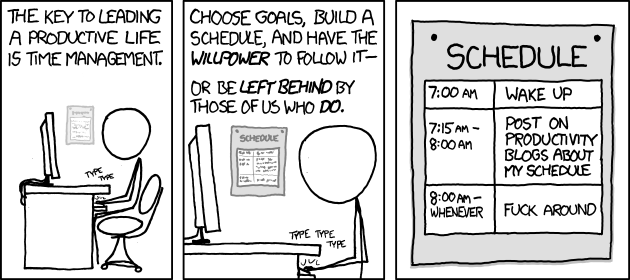
\includegraphics[scale=0.57]{comics/time_management}
\end{center}


%%%%%%%%%%%%%%%%%%%%%%%%%%%%%%%%%%%%%%%%%%%%%%%%%%%%%%%%%%%%%%%%%%%%%%%%%%%

\newpage
\section{Was ist überhaupt Informatik?}
\spaltenanfang
\spaltenanfang
Wie immer gibt es noch mehr Meinungen als unsere und eure zum Thema was Informatik ist.
Und da es an der Uni immer gut ist die Meinungen der Professoren zu wissen, haben wir sie mal dazu gefragt.
(Und mit wir meinen wir Grzegorz, der die Interviews damals gemacht hat. Danke Grzegorz!)

\begin{flushleft}\underline{Interview mit Prof. Schnitger} \end{flushleft}

\begin{description}

\item[Fachschaft] 

Was bedeutet für Sie der Begriff Informatik?

\item[Prof. Schnitger]
 
\textit{Wissenschaft der Information.}

\item[Fachschaft]

Was war Ihre Motivation Mathematik zu studieren?

\item[Prof. Schnitger]

\textit{Es ist immer klar worum es geht: Abenteuer im Kopf.}

\item[Fachschaft]

Was fasziniert Sie heutzutage an der Informatik?

\item[Prof. Schnitger]

\textit{Vieles beruht auf der Verarbeitung von Informationen: physikalische Prozesse, Steuerung durch Genom, ...}

\item[Fachschaft]

Welche Tipps können Sie aus Ihrer eigenen Zeit Erstsemestern für das Studium geben?

\item[Prof. Schnitger]

\textit{Arbeiten, arbeiten, ..., und Spaß haben.}

\end{description}
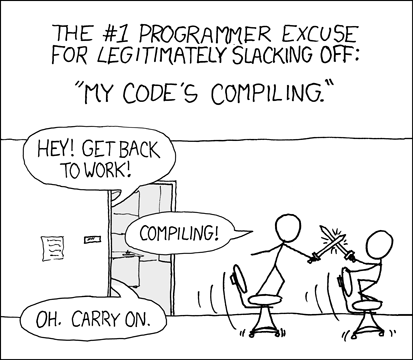
\includegraphics[width=0.95\linewidth]{comics/compiling.png}


\begin{flushleft}\underline{Interview mit Prof. Schmidt-Schauß} \end{flushleft}

\begin{description}

\item[Fachschaft] 

Was bedeutet für Sie der Begriff Informatik?

\item[Prof. Schmidt-Schauß]
 
\textit{Alles was mit  Berechnung, mit Rechnern und Informationsverarbeitung zu tun hat.}

\item[Fachschaft]

Was war Ihre Motivation Mathematik zu studieren?

\item[Prof. Schmidt-Schauß]

\textit{Mathematik war mein Interessengebiet. Mit Computern hatte ich zum ersten mal im vierten Semester zu tun im Numerik Praktikum.}

\item[Fachschaft]

Was fasziniert Sie heutzutage an der Informatik?

\item[Prof. Schmidt-Schauß]

\textit{Informatik bzw. Computer sind relevant in immer mehr Bereichen des Lebens, Technik und Wissenschaft.
Informatik ist eine junge Wissenschaft und es gibt dort noch zahlreiche offene und interessante Probleme zu lösen.}

\item[Fachschaft]

Welche Tipps können Sie aus Ihrer eigenen Zeit Erstsemestern für das Studium geben?

\item[Prof. Schmidt-Schauß]

\textit{Grundlagen der Informatik in jeder Form sind wichtig (nicht beschränkt auf die entsprechende Vorlesung). Später im Berufsleben gibt es so gut wie keine Zeit mehr, die Theorie, die jetzt leicht zu lernen ist, nochmals nachzuholen.}

\end{description}


\begin{flushleft}\underline{Interview mit Prof. Hedrich} \end{flushleft}

\begin{description}

\item[Fachschaft] 

Was bedeutet für Sie der Begriff Informatik?

\item[Prof. Hedrich]
 
\textit{Informatik ist die Wissenschaft der Informationsverarbeitung im Allgemeinen.
Sie ist durch die rasante Entwicklung in der Computertechnik zu einer sehr
bedeutsamen Wissenschaft geworden und weist damit sehr viele unterschiedliche, 
interessante Zweige auf. Von der Robotik bis hin zur Logik und Komplexitätstheorie.}


%\includegraphics[width=\linewidth]{comics/FuturamaComics/Comicsfinal/Studienwahl4voll}

\item[Fachschaft]

Was war Ihre Motivation Elektrotechnik zu studieren?

\item[Prof. Hedrich]

\textit{Während des Studiums konnte ich mein Interesse für die Computer (ich hab
in der Schule mit einem Commodore PET angefangen und mich dann in
die C64 Technik vertieft) mit dem für Elektrotechnik verbinden.
So kam es zu meinem Forschungsinteressen, den rechnergestützten Entwurf von
Schaltungen.}

\item[Fachschaft]

Was fasziniert Sie heutzutage an der Informatik?

\item[Prof. Hedrich]

\textit{Das weite Anwendungsfeld und besonders auch die großen
Gestaltungsmöglichkeiten, da Informatik ja inzwischen fast überall
zu finden ist. Speziell finde ich natürlich die technischen Entwicklungen
spannend z.B. den aktuellen Umstieg von Single-Prozessorsystemen auf
Multi-Cores bis hin zu 800 Prozessoren auf einer Grafikkarte für
jedermann.}

\item[Fachschaft]

Welche Tipps können Sie aus Ihrer eigenen Zeit Erstsemestern für das Studium geben?

\item[Prof. Hedrich]

\textit{Schauen Sie sich die Vorlesungen an. Es kann sowohl fachlich als auch
menschlich interessant sein. Ein guter Studienkommilitone hilft enorm,
sowohl bei der Auswahl der richtigen Veranstaltungen als auch während der
ganzen Lernerei. Und ein bisschen Entspannung bei einer Fete ist am Ende einer Woche
auch nicht verkehrt.}

\end{description}


%\includegraphics[width=\linewidth]{comics/FuturamaComics/Comicsfinal/Studienwahl5voll}

%\begin{flushright} Grzegorz \end{flushright}

\spaltenende




\spaltenende

\vspace{4mm}
\hspace{1cm}
\begin{center}
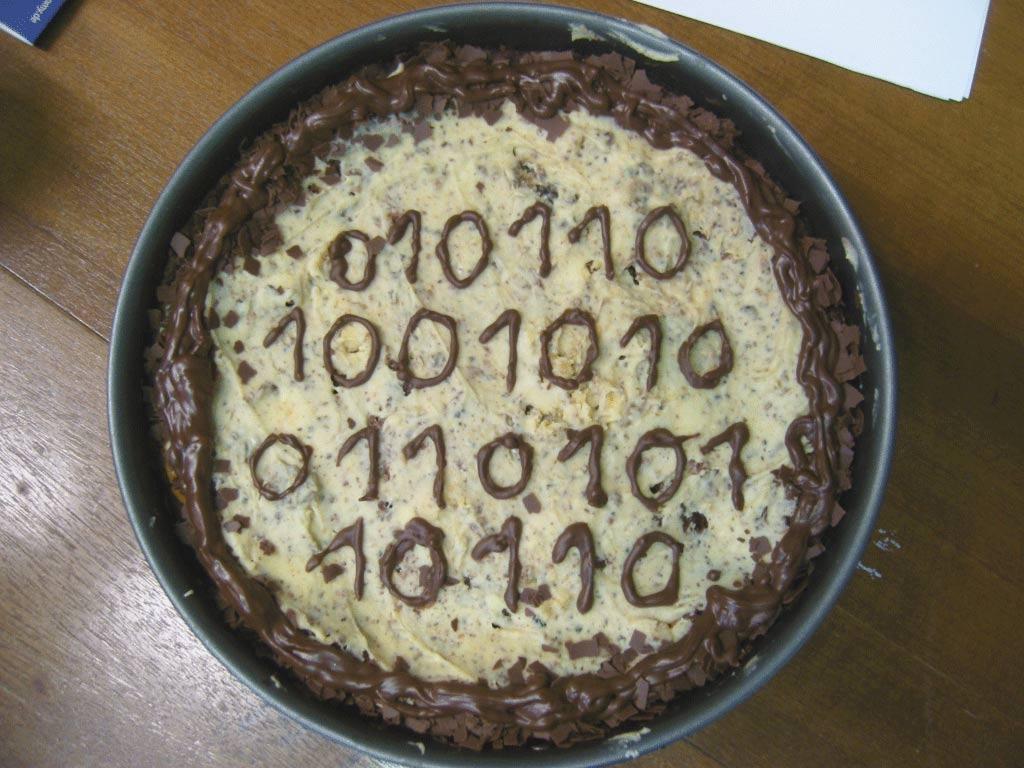
\includegraphics[scale=0.3]{bitmaps/101_kuchen}
\end{center}

%%%%%%%%%%%%%%%%%%%%%%%%%%%%%%%%%%%%%%%%%%%%%%%%%%%%%%%%%%%%%%%%%%%%%%%%%%%

\newpage
\section{Die Bibliothek am Institut für Informatik}
\spaltenanfang
Bibliothek, woran denkt man, wenn man diesen Begriff hört? Vermutlich an einen dunklen großen Raum mit vielen hohen Regalen aus Eichenholz mit einer ganzen Menge verstaubter Bücher darin, kleine Lesepulte mit grünen Lampen, eine alte Bibliothekarin, die am Eingang sitzt und über ihre Lesebrille schaut und an eine Stille, die ruhiger ist als fünf Minuten vor dem Urknall. Nun ja, auf manche Bibliothek mag das vielleicht zutreffen, aber ganz bestimmt nicht auf unsere Institutsbibliothek. Aber werfen wir zunächst einmal einen Blick ins Lexikon:\\

\begin{flushright}
\textit{Bi $\cdot$ bli $\cdot$ o\textasciiacute thek, Bi\textbar bli\textbar o\textbar thek~ \textless f.; -, -en\textgreater}

\textit{[grch. bibliotheke biblion „Buch“ + theke „Behältnis“] Büchersammlung, Bücherei; Raum od. Gebäude, in dem diese aufbewahrt wird. Die ältesten Bibliotheken des abendländischen Kulturkreises sind die babylonischen Sammlungen von Keilschrift-Tontafeln. Im griechischen Altertum dann Buchsammlungen in Alexandria und Pergamon. Im frühen Mittelalter waren Klöster die alleinigen Sammelstätten der Literatur, aus denen sich später dann die Universitätsbibliotheken entwickelten. [\dots]}
\end{flushright}

Und wenn man heute in so manche Unibibliothek geht, hat man immer noch das Gefühl, in einem Kloster zu sein. Aber wie schon gesagt, bei uns sieht das anders aus.\\

Die Bibliothek des Instituts für Informatik befindet sich im ersten Stock des Institutsgebäudes in der Robert-Mayer-Str. 11–15. Durch die große, rote Tür geht man in einen hellen, angenehmen Raum, der in der Regel von 09:00 Uhr bis 18:00 Uhr geöffnet ist. Hier findet man sicher nicht viele verstaubte Bücher (auch keine Tontafeln mehr, und Mönche sieht man auch eher selten), denn hier stehen viele der Bücher, die ihr für euer Studium braucht, und es lohnt sich immer, mal einen Blick hineinzuwerfen. Das sind natürlich vor allem Bücher aus den verschiedenen Bereichen der Informatik, aber auch Mathebücher, ein paar Physik- und Elektrotechnikbücher sowie viele der wichtigsten Fachzeitschriften. In der Regel findet man auch die von den Professoren zu den Veranstaltungen angefertigten Skripte als Kopiervorlage in der Bibliothek (obwohl es die Skripte oft auch im Internet gibt und ihr sie ausdrucken könnt).\\

In der Bibliothek steht Euch eine große Auswahl von Büchern aus allen Teilbereichen der Informatik zur Verfügung. Viele Studenten suchen die Bib auch zum Lernen und Arbeiten auf, wo die passenden Fachbücher sofort greifbar sind. Wenn ihr Euch jedoch in Lerngruppen zusammensetzen und unterhalten wollt, solltet ihr aus Rücksicht auf die anderen Studenten unser \textbf{Lernzentrum} nutzen. Wenn ihr durch den Haupteingang des Informatikgebäudes kommt, findet ihr es gleich links im Erdgeschoss.\\

Außer den Präsenzexemplaren kann man die Bücher auch für zwei Wochen ausleihen und mit nach Hause nehmen. Dazu müsst ihr in der Bibliothek Eure \textit{Goethe-Card} vorlegen (siehe Glossar auf S. \pageref{glossar}).\\

Wenn ein Prof. am Anfang der Vorlesung eine ganze Liste mit Büchern vorschlägt, ist es immer ganz gut, sich nicht gleich alle zu kaufen, sondern sich erstmal die Bücher zu leihen, mal reinzuschauen und damit zu arbeiten. So kann man feststellen, ob man mit dem Buch überhaupt etwas anfangen kann. Es sind zwar nicht immer alle der vorgeschlagenen Bücher in der Bibliothek zu finden und natürlich auch nicht 300 bis 400 Exemplare, so dass jeder eins mit nach Hause nehmen kann, aber meistens findet man ein Buch, das einem weiterhilft.\\

Sollte man mal ein Buch nicht auf Anhieb finden, so kann man im Internet auf der Bibliothekshomepage oder direkt auf den Recherche-Rechnern in der Bibliothek danach suchen, wer lieber mit dem eigenen Notebook sucht, kann auch das hauseigene WLAN nutzen; wenn das auch nicht hilft oder man eigentlich gar nicht so genau weiß, was man sucht, kann man ruhig auch mal einen von den Menschen fragen, die dort arbeiten.\\

Andere Bibliotheken, die noch hilfreich sein könnten:

%%%%%%%%%%
\begin{description}
\item[Die Bereichsbibliothek der Mathematik.] Im Mathegebäude, im obersten, dem vierten, Stock. Hier stehen, welch’ Wunder, vor allem Mathebücher und -skripte. Hat den Charme eines Krankenhausflures, eine der Bibliotheken, in der man besser keine Stecknadel fallen lässt, bestimmt direkt aus einer Klosterbibliothek hervorgegangen (s.o.).

\item[Die Universitätsbibliothek.] Direkt an der U-Bahn-Haltestelle Bockenheimer Warte, nicht zu übersehen. Hier gibt es viele Bücher mit Themen aus anderen Fachbereichen. Die großen Säale sind gut geeignet, um sich zum stillen Lernen zurückzuziehen.

\item[Die Deutsche Bibliothek.] Sie ist die zentrale Archivbibliothek der Bundesrepublik Deutschland. Sie sammelt alle deutschsprachigen Veröffentlichungen des In- und Auslandes seit 1945, ferner Übersetzungen deutscher Werke, fremdsprachige Werke über Deutschland und Exilliteratur der Jahre 1933 -- 1945.

\item[Die Technische Bibliothek.] Zu finden in der Waldschmidtstraße 39, kann man sie von der U-Bahnstation Zoo nach einem dreiminütigen Fußmarsch erreichen. In Sachen Unhöflichkeit ist sie unübertroffen, und die Ausleihbeschränkung auf maximal fünf Medien macht sie auch nicht sympathischer, geschweige denn die Öffnungszeiten (Mo, Do: 13 -- 19 Uhr; Di, Mi, Fr: 13 -- 17 Uhr). Aber man findet dort Bücher, die man in den oben genannten Bibliotheken eventuell nicht findet.

\item[Die Bibliotheken der anderen Fachbereiche.] Wo diese sind und was ihr da so findet, erfahrt ihr am besten von den Angehörigen der entsprechenden Fachbereiche.
\end{description}
%%%%%%%%

\begin{flushright} Björn\end{flushright}
\spaltenende

%\begin{minipage}[t]{\linewidth}
\begin{center}
\vspace{7mm}
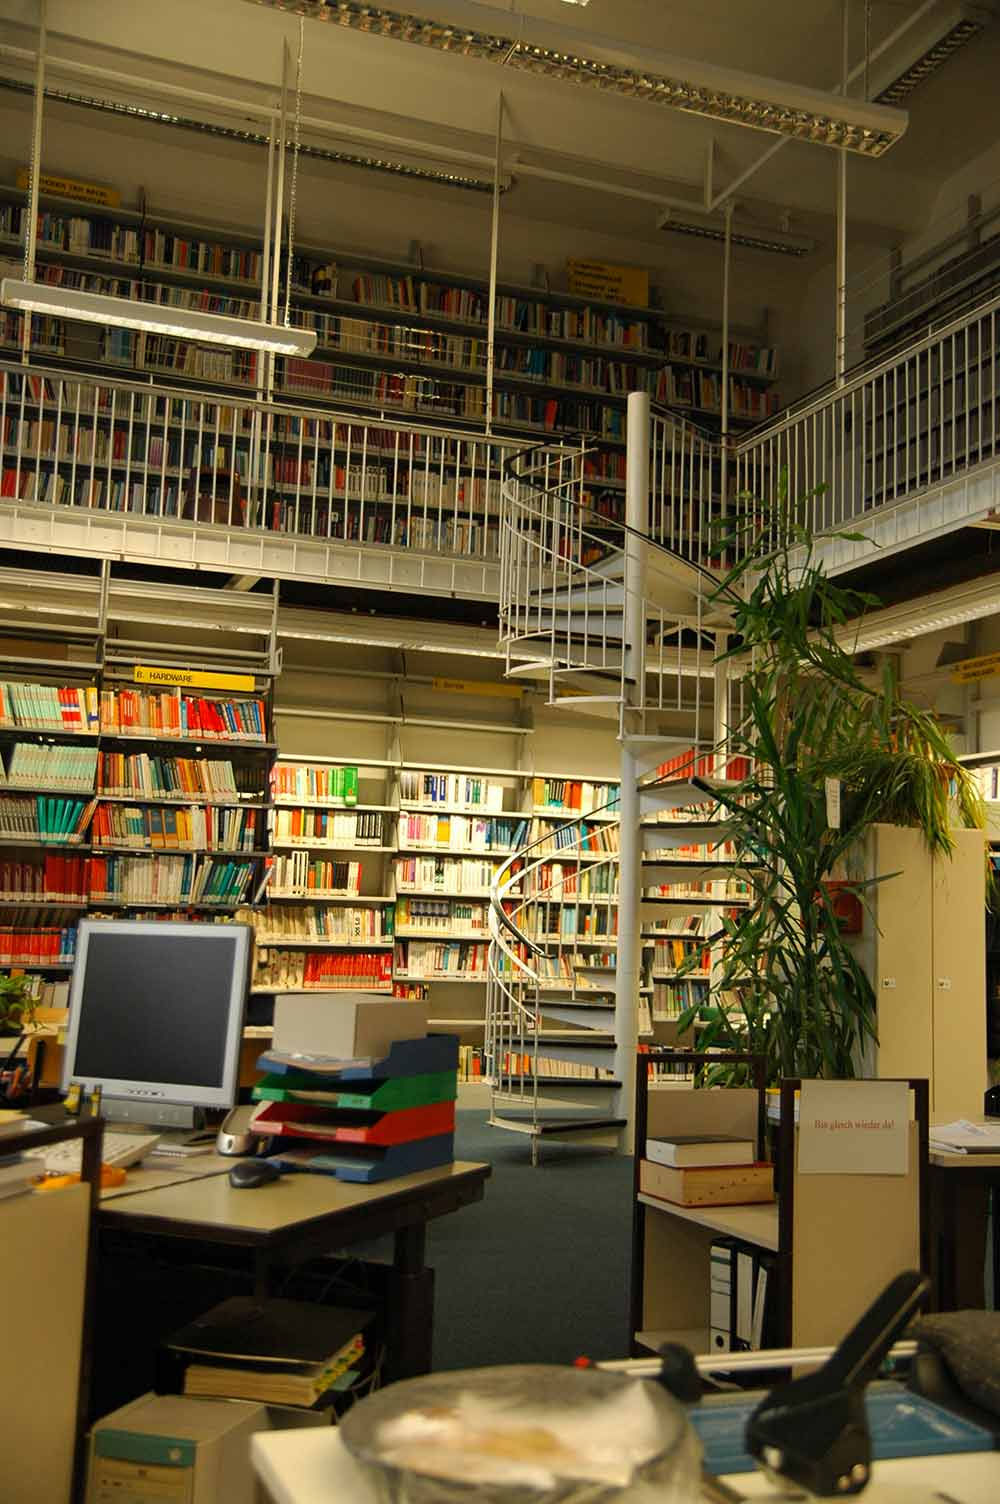
\includegraphics[width=85mm]{fotos/bib}
\end{center}
%\end{minipage}



%%%%%%%%%%%%%%%%%%%%%%%%%%%%%%%%%%%%%%%%%%%%%%%%%%%%%%%%%%%%%%%%%%%%%%%%%%%

\section{Fachschaftsarbeit… was ist das eigentlich?}

%das Label setzen wir
\label{fachschaftsarbeit}

\spaltenanfang
%\includegraphics[width=\linewidth]{comics/FuturamaComics/Comicsfinal/jointheFachschaftfull}
Schaut man in das hessische Hochschulgesetz (HHG), so erfährt man, dass sich „die Fachschaft aus allen Studierenden eines Fachbereichs“ zusammensetzt. Fragt man auf dem Campus rum, so erfährt man vielleicht, dass „Fachschaftler“ Leute sind, die an der Uni (politisch) aktiv sind. Aber was macht so ein „Fachschaftler“ denn nun eigentlich genau? Fangen wir doch einfach mal mit dem an, was du gerade in der Hand hältst:

\begin{itemize}
 \item Irgend jemand hat diese Ausgabe der „Don‘t Panic!“ erstellt, Ideen entwickelt, Bilder gesetzt und Texte geschrieben. Das waren Fachschaftler.

 \item Irgend jemand hat Freiwillige als OE-Tutoren rekrutiert, Frühstück besorgt, sich um Sponsoren bemüht und diese ganze Orientierungseinheit organisiert. Das waren Fachschaftler.
 
 \item Irgend jemand bereitet (teils mit der Hilfe der Professoren) Sommer-, Weihnachts-, Halloween- und sonstige Feste vor und sorgt dafür, dass man Essen und Trinken kaufen kann. Das sind Fachschaftler.

 \item Irgend jemand versucht tagtäglich, deine Interessen gegenüber Professoren und anderen Bösewichten durchzusetzen. Das sind Fachschaftler.

 \item Irgend jemand ist für dich da, wenn es in Veranstaltungen beschissen läuft, unfaire Bedingungen vorhanden sind, du Fragen zu Studium, Prüfungsmodalitäten oder diversen Veranstaltungen hast. Das sind Fachschaftler.

 \item Irgend jemand leiht dir ein Ohr, wenn du eine Studienberatung willst. Das sind Fachschaftler.

 \item Irgend jemand antwortet dir, wenn du Fragen an die E-Mail-Adresse \emailfachschaft schickst. Das sind Fachschaftler.
\end{itemize}

Okay, damit wäre schonmal grob umrissen, was wir Fachschaftler so tun. Aber was heißt das denn nun genau?


Nehmen wir doch mal das Beispiel „nicht geregeltes Anwendungsfach“. Auch wenn Du hoffentlich bald eine recht breite Auswahl an Anwendungsfächern haben wirst, möchtest du vielleicht doch etwas anderes machen. Egal, ob du nun erst zum Prüfungsamt gehst, um dir die Prozedur erklären zu lassen, oder gleich zu uns kommst, früher oder später landet dein Antrag in einem Gremium, genannt „Institutsrat“ oder auch „Direktorium“. In diesem Gremium werden alle informatikspezifischen Angelegenheiten von Professoren, wissenschaftlichen, administrativ-technischen Mitarbeitern und Studierenden, also Fachschaftlern, diskutiert und beschlossen. Im Zweifelsfall erklären also deine Fachschaftler hier den Professoren, warum deine Wahl eines Anwendungsfachs sinnvoll ist.


Ein anderes Beispiel wäre der Lehr- und Studienausschuss (kurz LuSt). In diesem Gremium wird unter anderem das Lehrangebot erstellt. Auch hier sitzen Professoren mit deinen Fachschaftlern zusammen und achten darauf, dass die Professoren auch ihre Lehrverpflichtung erfüllen, dass in den einzelnen Bereichen genug Lehre vorhanden ist, dass es genug Praktika und Seminarplätze gibt, alles in allem also, dass dein Studium halbwegs studierbar bleibt. Fachschaftler schauen sich auch immer wieder um, was außerhalb so alles los ist, und machen Vorschläge, welche Externen man dazu einladen könnte, um bei uns eine Veranstaltung durchzuführen.


Fachschaftler sind es auch, die neue Entwürfe für die Bachelor-Ordnung durchsehen und kommentieren. Denn man muss sowas einfach aus Studierendensicht durchgehen, um zu merken, dass das Ding so nicht studierbar ist.


%\renewcommand{\labelitemi}{\textendash}

Und nicht zu vergessen, sind es auch Fachschaftler, die in den ganzen Gremien deine Beschwerden weitergeben und deine Wünsche vertreten. Wie du siehst, gibt es für Fachschaftler an allen Ecken und Enden etwas zu tun, und um all das zu tun, brauchen wir DICH!

\begin{itemize}

\item Wir brauchen DICH, um uns Bescheid zu geben, wenn in einer Veranstaltung etwas nicht so läuft, wie es sollte.

\item Wir brauchen DICH im nächsten Jahr, um als OE-Tutor die neuen Erstsemester zu betreuen.

\item Wir brauchen DICH, damit du im kommenden Frühjahr zur Wahl gehst.
\item Und wir brauchen DICH, damit einfach mal bei unseren Gremientreffs vorbeikommst, und mal schaust, ob du uns nicht unterstützen willst.
\end{itemize}

Also, wenn du Lust hast, dann schau doch einfach mal donnerstags gegen 16:00 Uhr bei uns vorbei. Und wenn du Fragen hast oder es Probleme gibt, dann zögere nicht, uns anzusprechen. Wenn im neuen Fachschaftsraum (direkt hinter dem Lernzentrum) niemand anzutreffen ist, dann vielleicht in der Bibliothek. Oder einfach per E-Mail: \emailfachschaft

\renewcommand{\labelitemi}{$\bullet$}

\begin{flushright} Alexander \end{flushright}



\spaltenende

\vspace{20mm}
\begin{center}
	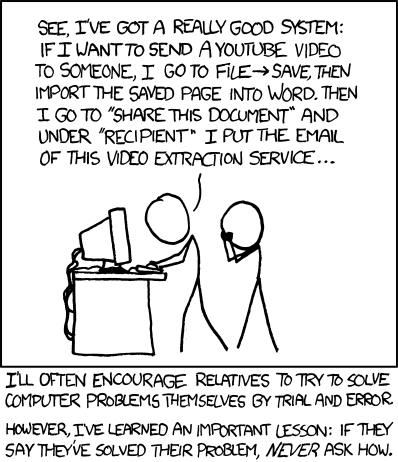
\includegraphics[scale=1.0]{comics/workaround}
\end{center}

\newpage

%%%%%%%%%%%%%%%%%%%%%%%%%%%%%%%%%%%%%%%%%%%%%%%%%%%%%%%%%%%%%%%%%%%%%%%%%%%

%\section{Der 3-Sterne-Koch}

%{
%\setlength{\fboxsep}{0pt}
%\setlength{\fboxrule}{1.25pt}

%\begin{center}
%\vspace{35mm}
%\fbox{\includegraphics[scale=0.6]{comics/3_sterne_koch/01}}\\
%\vspace{5mm}
%\fbox{\includegraphics[scale=0.6]{comics/3_sterne_koch/02}}\\
%\vspace{5mm}
%\fbox{\includegraphics[scale=0.6]{comics/3_sterne_koch/03}}\\
%\vspace{5mm}
%\fbox{\includegraphics[scale=0.6]{comics/3_sterne_koch/04}}\\
%\vspace{5mm}
%\fbox{\includegraphics[scale=0.6]{comics/3_sterne_koch/05}}\\
%\vspace{5mm}
%\fbox{\includegraphics[scale=0.6]{comics/3_sterne_koch/06}}\\
%\vspace{5mm}
%\fbox{\includegraphics[scale=0.6]{comics/3_sterne_koch/07}}\\
%\end{center}

%}

%%%%%%%%%%%%%%%%%%%%%%%%%%%%%%%%%%%%%%%%%%%%%%%%%%%%%%%%%%%%%%%%%%%%%%%%%%%

\section{The Rise of the Robots: die Robocup-AG}

\spaltenanfang
\spaltenanfang
Wir schreiben das Jahr 2050. Im Madison Cube Garden stehen sich 11 menschliche und 10 Roboter-Fußballer gegenüber. Moment, 10? Da fehlt doch einer! Aha, Bender steht rauchend und trinkend auf der VIP-Tribüne und klaut Schmuck und Uhren!
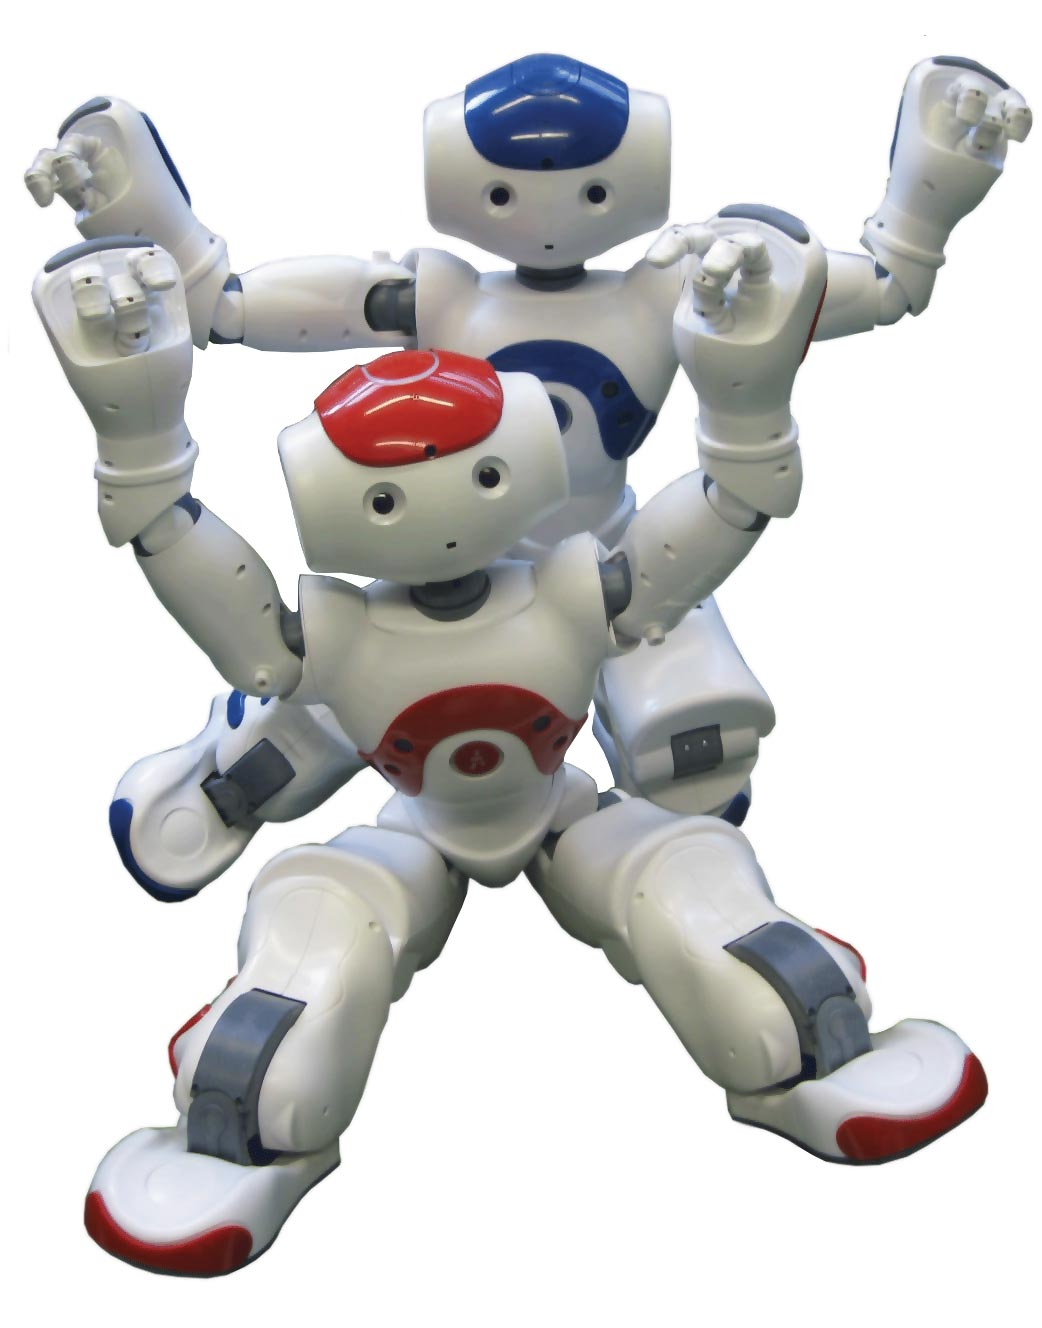
\includegraphics[width=8cm]{bilder/robocup1}

So oder ähnlich oder komplett anders könnte die Zukunft aussehen, wenn DU bei unserem Team mitmachst!

Doch blicken wir zurück ins Jahr 2009, wo alles seinen Anfang fand. Mittlerweile hat schon fast jede Erd-Universität eigene Prototypen, unter anderem auch die Robocup-AG der Universität Frankfurt. Die Vorform von Bender, Nao genannt, hat noch bessere Manieren und sieht relativ harmlos aus, ist aber leider auch noch ziemlich unfähig. Und hier kommt das Team Bembelbots ins Spiel, die Studenten der Robocup-AG, die ihm Leben einhauchen. Unter der Schirmherrschaft des Joint Robotics Lab (JRL) arbeiten wir ständig an der Verbesserung von Naos Fähigkeiten.

Unabhängig vom Kenntnisstand findet sich bei uns für jeden eine Aufgabe, der Robocup bietet für jeden Teilbereich der Informatik spezielle Herausforderungen. So kann man sich entscheiden, ob man mit Hilfe von Bildverarbeitung, Bewegungsoptimierung, Künstlicher Intelligenz oder aber auf einem ganz anderen Weg unseren Robotern zum Erfolg verhilft.

Und mit etwas Glück erfüllen wir das oben aufgeführte Szenario von Professor Farnsworths ``Was wäre, wenn?''-Maschine und lassen unsere Roboter wirklich irgendwann gegen menschliche Gegner antreten. Wenn du interessiert bist, mitmachen oder einfach mal reingucken willst, bist du herzlich eingeladen, in der Robert-Mayer-Straße 8, Raum 09a (im Kellergeschoss) vorbeizukommen, oder du besuchst unsere Internetseite zum Robocup/JRL:
 
\url{http://www.bembelbots.de}

Hier findest du neben Infos zum Robocup auch andere studentische Projekte des Joint Robotics Lab. 
\spaltenende

\includegraphics[width=0.8\textwidth]{bilder/Bembelbots}

\spaltenende
\vspace{4mm}
\begin{center}

\includegraphics[scale=0.25]{bitmaps/Bembelbots}
\end{center}
\newpage

%%%%%%%%%%%%%%%%%%%%%%%%%%%%%%%%%%%%%%%%%%%%%%%%%%%%%%%%%%%%%%%%%%%%%%%%%%%

\section{Internet – LOL – Internet!}

%\spaltenanfang
\subsection*{How to: W-LAN}

Du bist nun stolzes Mitglied der Goethe-Universität Frankfurt oder schlichtweg begeisterter Interessent für unseren
Fachbereich „Informatik“? Jetzt stellt sich dir nach einer Stunde frustriertem Haareraufen die Frage: „Haben die Freaks
hier kein Internet!?“

Doch klar, aber wir wären doch keine Fachidioten, wenn der Zugang jedem benutzerfreundlich
zugeschoben würde. Deshalb haben wir es uns zur Aufgabe gemacht, den Umstand der Router-Suche, das Feilschen um
notwendige Dateien \& die Durchführung einer Serverwartung unangekündigt genau dann zu starten, wenn du es am wenigsten
erwartest; oder zumindest ließen sich so einige unglaubliche Phänomene ansatzweise begründen.

\begin{center}
	
\includegraphics{bitmaps/network-wlan-icon}
\end{center}
\vspace{-5mm}

%%%%%%%%%%%%%%%%%%%%
\subsection*{Minimale Anforderungen}

Ohne dich gleich überfordern zu wollen, musst du dir darüber im Klaren sein, dass du ohne einen Laptop, oder ein „Mobile
Device“ nicht weit kommst. Sollte beides nicht zur Hand sein, ließ erst einmal beim Punkt „W-LAN Versorgung“ weiter.
Falls du die Zeile noch nicht verlassen haben solltest: Um dich mit einem unserer Router zu verbinden, benötigst du
einen HRZ-Account.

\begin{fancyblock}{HRZ?}
	Das Hochschulrechenzentrum stellt euch verschiedene Services zur Verfügung.\\
	Unter anderem den Internetzugang! Mit deiner Erstimmatrikulation hast du deine\\
	HRZ-Login-Daten erhalten, die dir als Identifikationsschlüssel dienen.
\end{fancyblock}

Auf dem Campus müsste dein Rechner verschiedene Netzwerke finden, u.a. FLUGHAFEN, eduroam und FREIFLUG. Was sich auf den
ersten Blick nicht erkennen lässt; hierbei handelt es sich um das gesuchte Angebot an dich eine W-LAN Verbindung
aufzubauen.

Diskutieren wir nicht über die Namen und treffen eine beliebige Wahl. In der unteren, rechten Ecke deines
Bildschirms erscheint nun ein kleines Fenster, in dessen Spalten du dein HRZ-Login und -passwort eintippst (bei FREIFLUG
erfolgt die Authentifizierung über den Browser\footnote{Das Formular erscheint beim Aufruf der ersten Webseite.}).

Das funktioniert sowohl für deinen Laptop, als auch für dein Handy, IPad, etc.

%%%%%%%%%%%%%%%%%%%%
%\subsection*{Hey, ich bin aber kein Student an dieser Uni!}
%
%Ausnahmsweise darfst du trotzdem sitzen bleiben.\\
%Ließ einfach die Erläuterungen zum Vorsemesterkurs.
%
%%%%%%%%%%%%%%%%%%%%
\subsection*{RBI}

Um die Unirechner zu verwenden, die sich in den Fischerräumen finden lassen, benötigst du wiederum andere Login-Daten,
diese werden dir von der RBI zur Verfügung gestellt.

\begin{fancyblock}{RBI?}

Die Rechnerbetriebsgruppe Informatik besteht aus einer Hand voll Linux-Fanatikern, die ihren Sitz
im Keller des Institutsgebäudes beziehen. Solltest du einmal Probleme mit der Internetverbindung haben, folge einfach
der Treppe nach unten ins Dunkel...
\end{fancyblock}

Wenn du am Vorsemesterkurs Informatik teilgenommen hast, wurden dir zu Beginn die entsprechenden Zugangsdaten
ausgeteilt, mit denen du auf die RBI-Rechner zugreifen kannst. Ändere bitte bei der ersten Anmeldung dein Passwort \&
denk nicht einmal darüber nach „Gandalf“ zu verwenden; hier ist ein wenig Kreativität gefordert! Merke: Unsichere Passworte können zur Accountsperrung führen! 

Deinen RBI-Account benötigst du nicht nur für die Unirechner, sondern auch um das RBI-Netzwerk nutzen zu können und
später für das Praktikum. Im Fall, dass du den Vorsemesterkurs verschwitzt hast, begebe dich einfach in den Keller des
Institutsgebäudes und bitte die Mitarbeiter der RBI dir ein Konto zu eröffnen.

\begin{fancyblock}{WARNUNG!}

Bevor dir deine Daten ausgehändigt werden, wirst du dazu angehalten eine entsprechende
Zustimmungserklärung zu unterzeichnen, in der du dich dazu verpflichtest, deine Daten geheim zu halten. Sollte mit
deinem Account Unfug getrieben werden, kommen wir auf dich zurück!
\end{fancyblock}

\begin{fancyblock}{RBI-Netzwerk?}

Parallel zum HRZ bietet die RBI ebenfalls  den WLAN-Zugriff über ein eigenes Netzwerk an.
Sollte irgendwann ein HRZ-Access Point durch 20 andere Studierende überlastet sein, bleibt dir noch
der Ausweg zum OpenVPN Netzwerk der RBI zu wechseln.
\end{fancyblock}

%%%%%%%%%%%%%%%%%%%%
\subsection*{OpenVPN}

Dein RBI-Account ist nicht nur für die Fischerräume notwendig, sondern ermöglicht dir auch innerhalb des
Institutsgebäudes (zzgl. Matheturm) den Zugang zu einem weiteren Netzwerk.

Hier kommst du mit deinen Daten allein leider nicht mehr weiter:
\begin{enumerate}
	\item Wähle das OpenVPN Netzwerk aus, öffne deinen Browser und rufe eine beliebige Seite auf.

	Bevor du die Verbindung im ganzen Ausmaß nutzen kannst, bist du gezwungen dir einige Dateien für dein Betriebssystem herunterzuladen.
	\item Ist dir der Prozess geglückt, starte bitte das beinhaltete OpenVPN GUI Programm mit Administratorrechten (wichtig!).
	\item Vollziehe einen Rechtsklick auf das zugehörige Icon in deiner Taskleiste und wähle „connect“, im Anschluss wirst du dazu aufgefordert
	deine RBI-Daten einzutippen.

	Versuche es erst gar nicht mit den HRZ-Daten. Der RBI-Login beinhaltet deinen Namen (nicht	zu verwechseln)!
	\item  Bei Bedarf bitte nicht verzweifeln, bediene dich des „Reconnect's“!
\end{enumerate}

\begin{fancyblock}{Der OpenVPN-Bonus}

In einigen Stöcken des Matheturms, wo der Signal von HRZ-Netzwerken sehr schwach ist,
lässt sich mit OpenVPN eine Internetverbindung herstellen. Ihr müsst hierzu die IP-Adresse in der Konfigurationsdatei
austauschen. Eine Anleitung findet sich in eurem Browser, wenn ihr versucht auf das Netzwerk zuzugreifen und eine
beliebige Webseite aufzurufen..
\end{fancyblock}

%%%%%%%%%%%%%%%%%%%%
\subsection*{W-LAN Versorgung \& Fehlerbehebung}

\begin{itemize}
	\item \textbf{Ich besitze keinen eigenen Laptop!}

	Nutze bitte einen der lokalen Unirechner in den Fischerräumen.
	
	\item \textbf{Mein Rechner findet einfach kein Netzwerk!}

	\begin{tabular}{p{0.2\linewidth}p{0.77\linewidth}}
\rule{0pt}{2ex} 
	Fischerräume: & Nutze die lokalen Rechner, dafür sind sie da!\\
\rule{0pt}{4ex} 
	Mathe-Turm: & Hier sind nicht alle Stöcke mit dem WLAN versorgt.

	Melde dich mit den Beschwerde, bitte, bei der Mathe-Fachschaft: fachschaft@math.uni-frankfurt.de\\
\rule{0pt}{4ex} 
	Lernzentrum, &  Finde oben ein weißes Access Point.  Sollte darauf ein grünes oder\\
\rule{0pt}{0ex} 
	Student Lounge, & ein blaues LED leuchten, liegt das an deinen WLAN-Einstellungen.\\
\rule{0pt}{0ex} 
	SR11 und SR307: & Sollte das LED rot leuchten, teile das dem HRZ-Team mit:

	wlan-fragen@rz.uni-frankfurt.de\\
\rule{0pt}{4ex} 
	Magnus, SR9: & Melde dich mit deiner Beschwerde bitte bei der RBI.\\
\rule{0pt}{4ex} 
	Weitere Infos: & \url{www.rz.uni-frankfurt.de/campusnetz/wlan/flugplatz/cb.html}
	\end{tabular}
\end{itemize}

\begin{fancyblock}{OpenVPN funktioniert plötzlich nicht mehr!}
Entweder du hast die falsche IP-Adresse in deiner Konfigurationsdatei auskommentiert,
oder bei der letzten Reinigung deines Rechners ging eine wichtige Datei verloren.
In diesem Fall empfiehlt es sich das Paket für dein Betriebssystem erneut downzuloaden.
\end{fancyblock}

\begin{flushright}Sabrina \& Pavel \end{flushright}

%\vspace{3mm}
%\begin{center}
%	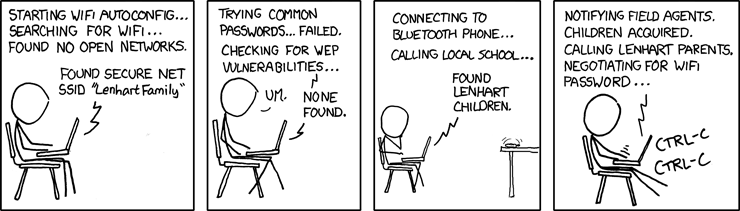
\includegraphics[scale=0.42]{bitmaps/zealous_autoconfig}
%\end{center}

%\spaltenende
\newpage


%%%%%%%%%%%%%%%%%%%%%%%%%%%%%%%%%%%%%%%%%%%%%%%%%%%%%%%%%%%%%%%%%%%%%%%%%%%

\section{Windows Lizenzen + weiteres Software für Informatiker}

Wenn du für dein Studium im Fachbereich 12 Windows oder ein anderes Programm von Microsoft brauchst\footnote{Word, Excel, Access und Spiele von Microsoft sind ausgeschlossen}, aber als ein armer Student dir ein solches Luxusprodukt nicht leisten kannst, habe keine Angst: Wir nehmen an Programm Dreamspark Premium\footnote{Weitere Infos: \url{http://www.microsoft.com/germany/msdn/academic/dreamspark/}} teil, wodurch dieses Software für die Studierenden kostenlos verfügbar ist. % der letzte Satz ist eine Zitat von der offiziellen Webseite von Dreamspark Premium

Die Lizenzen werden von Herrn Plass aus der RBI verwaltet. Man findet ihn im Raum 014a im Keller des Informatik-Gebäudes.
Die Vergabe der Lizenzen erfolgt über zwei unterschiedliche Wege:

\begin{noindItemize}
	\item Web-Portal (ELMS)
	\item Manuelle Verwaltung
\end{noindItemize}

% ### Das würde der Lizensierungsbedingungen von Microsoft widersprechen: ###
%Er würde dir \textbf{die Lizenznummer} für diejenige Windows-Distribution geben, \textbf{die du brauchst} und dementsprechend nachfragst, falls sie bei ihm vorhanden ist.
%Und komme zu ihm, bitte, nicht mit den Wörtern "Geben Sie mir alle Lizenzen, die Sie haben!", da jede Lizenz von der RBI gekauft werden muss, und es kein großer Sinn macht, für diejenige Programme Geld auszugeben, deren Namen du nicht kennst und die du also niemals im Leben tatsächlich benutzen wirst.

\begin{center}
	
\includegraphics[scale=0.35]{bitmaps/win8logo}
\end{center}

\subsection{Web-Portal (ELMS)}

Wenn du beim Herrn Plass nach dem Zugang zum Web-Portal von Dreamspark Premium \textbf{freundlich} nachfragst, wird er dich nach deiner Uni-E-Mail-Adresse nachfragen, wodurch bestätigt werden kann, dass du bei uns studierst.

In Kürze darauf bekommst du eine E-Mail mit den Logindaten zum Portal. Dort kannst du dann sowie die Distributionen der Softwareprodukte herunterladen, als auch die Lizenzen für dich generieren lassen.

Momentan sind im ELMS \textbf{163 (!)} Produkte verfügbar, darunter Windows 8 Professional, Windows~7 Professional, Visual Studio 2012, Visio 2013, Access 2013 usw.

Dieser Verfahren macht das Erhalten von Lizenzen und Distributionen unkompliziert und nach einmaliger persönlicher Meldung bis zum Ende des Studiums von zu Hause möglich.

\subsection{Manuelle Verwaltung}

RBI verwaltet die Lizenzen zu einigen insbesondere populären Produkten auch manuell. Wenn du \textbf{freundlich} nachfragst, gibt Herr Plass dir einen \textbf{Produktschüssel} für eine entsprechende Lizenz, wenn die Lizenz, \textbf{die du brauchst,} da ist.
% Microsoft darf nur die Liste der E-Mails zwecks Kontrolle, dass Lizenzen nicht verkauft werden, einsehen, also ist die Bemerkung irrelevant.
%Außerdem gibt es da alle Lizenzen aus dem Microsoft DreamSpark Premium Programm (ehemaliges MSDN-AA) so anonym wie möglich (Microsoft darf einmal im Jahr die Daten einsehen aber nicht kopieren oder speichern).

Diese Verwaltungsart ist für die Fälle sinnvoll, wo man aus irgendwelchen Gründen mehrere Lizenzen zu einem populären Softwareprodukt studienbedingt braucht (z.B. zwecks Analyse der gleichzeitigen Ausführung zweier Virtuellen PCs).

Dadurch Wer da aber unbedingt mit den Worten "Gib so viele Lizenzen, wie du hast!" 20 Lizenzen auf einmal haben will, sorgt nur dafür, dass solche Angebote in Zukunft nicht mehr von der Uni bezahlt werden und euch kostenlos zur Verfügung gestellt werden. Also nutzt das Angebot, aber nutzt es nicht aus!

Natürlich reicht die Lizenznummer für die Installation nicht. Du brauchst also noch ein \textbf{Installationsmedium}. Bei der RBI werden nicht Hunderte von CDs und DVDs gelagert. Jeder brennt sich eins selbst (das ist auch völlig legal, wen das interessiert ;)).

Die RBI hat normalerweise ein Distributions-CD zu jedem Programm, das du für ein paar Tage zum Kopieren ausleihen könntest.
Als eine Alternative für die Windows-Betriebsysteme, die sonst mehrmals täglich ausgeliehen wären, kannst du die bereits angefertigten Images\footnote{Digitalisierte Versionen der CDs und der DVDs} aus dem RBI-Netzwerk verwenden:
\begin{wrapfigure}[12]{r}{0.5\textwidth}
     \vspace{12mm}
   \begin{center}
     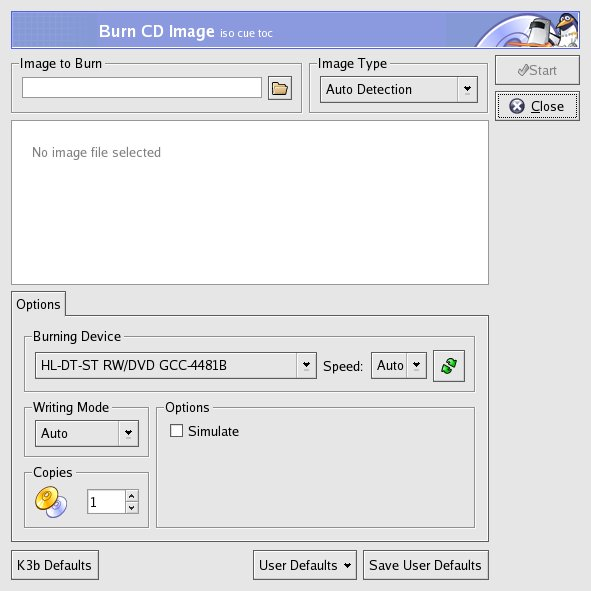
\includegraphics[scale=0.39]{bitmaps/gimp_brennen4}
   \end{center}
\end{wrapfigure}
\begin{enumerate}
\item Hole dir ein [DVD-]Rohling
\item Logge dich an einem der RBI-PCs ein (z.B. in den Fischerräumen)
\item Starte \texttt{k3b} z.B. in der Konsole
\item Gehe im Menü zu\\"Tools"'$\to$"Burn CD Image".

\item Nun muss du dass Image auswählen welches du brennen möchtest:\\
Klicke auf den ''wähle Datei'' Knopf 
\includegraphics[scale=0.5]{bitmaps/gelbe_ordner}, im Bereich ''Image to Burn'' und schau in diesem Ordner nach:

\begin{center}
	\framebox{ \textbf{ \textsf{/opt/rbi/ms\_windows\_iso/} } }
\end{center}
\item Danach wird die Isodatei überprüft. Das wird ein paar Sekunden dauern.

	Sobald dieser Prozess fertig ist, kann man auf den ''Start" Knopf klicken und damit das Brennen starten.

\end{enumerate}

Alternativ kannst du diese Images auf dein USB-Stick kopieren und bequem zu Hause brennen (zum Brennen von Images unter Windows kann man dafür das kostenlose Programm ImgBurn\footnote{\url{http://www.imgburn.com/}} verwenden).

\begin{flushright}Pavel und Jonathan \end{flushright}


\newpage
\begin{center}
	\ThisCenterWallPaper{0.82}{comics/tech_support_cheat_sheet}
\end{center}

%%%%%%%%%%%%%%%%%%%%%%%%%%%%%%%%%%%%%%%%%%%%%%%%%%%%%%%%%%%%%%%%%%%%%%%%%%%

\newpage
\section{Wichtige Adressen und Informationen}

\spaltenanfang
\subsection*{Deine Fachschaft}

\url{http://fs.cs.uni-frankfurt.de/}\\
\url{http://fs.cs.uni-frankfurt.de/forum/}\\
\emailfachschaft

\subsection*{Dein Fachbereich}

Fachbereich Informatik und Mathematik (12)\\
Institut für Informatik\\
Robert-Mayer-Straße 11–15\\
60054 Frankfurt\\

\begin{tabular}{ll}
Institutssekretariat & 798 – 23325 \\
Informatik-Bibliothek: & 798 – 22287\\
Informatik-Prüfungsamt: & 798 – 28279\\
Informatik-Studienberatung: & \\
~~~Prof. G. Schnitger & 798 – 28326\\
%~~~und die Fachschaft & 798 – 23933\\
\end{tabular}

\subsection*{Informationssystem}

Verwaltung Deiner persönlichen Daten rund ums Studium:

\begin{center}\url{http://go.uni-frankfurt.de}\end{center}

Vorlesungsverzeichnis:

\begin{center}\url{http://qis.server.uni-frankfurt.de}\end{center}


\subsection*{Der AStA}

Die Langform lautet Allgemeiner Studenten-Ausschuss; politisch korrekt nennt er sich auch meistens Allgemeiner Studierenden-Ausschuss. Der AStA ist die (leider nur von einer kleinen Minderheit) gewählte studentische Vertretung der gesamten Studierendenschaft, also aller Studierender der Universität. Der AStA hat verschiedene „Referate“, die sich mit speziellen Bedürfnissen von Teilen der Studierendenschaft oder auch besonderen Angeboten für eben selbige beschäftigen.

\paragraph{AStA-Büro}~\\
Studentinnenhaus, Mertonstr. 26–28, Raum B1\\
798 – 23181\\
Öffnungszeiten: Mo - Fr 9:30 -- 13:00 Uhr

\paragraph{Rechts- und BaföG-Beratung}~\\
Raum B7\\
798 – 23175 oder 798-33098\\
Bockenheim:\\
Mo, Di, Fr.: 10.00 - 12.00 Uhr
Mo, Di, Mi und Do : 13.00 - 15.00 Uhr


\paragraph{Sozialreferat}~\\
Raum B7\\
Beratung: Mo 12:00 -- 13:00 Uhr\\
Mi 12:00 -- 13:00 Uhr\\
Fr 13:00 -- 14:00 Uhr


\paragraph{BAföG}~\\
Wer wieviel BAföG bekommt, können wir hier natürlich nicht schreiben, aber durch die letzten Gesetzesänderungen lohnt sich eigentlich für Jeden der Weg ins BAföG-Amt.

\paragraph{Amt für Ausbildungsförderung}~\\
Neue Mensa, 4. Stock, Vorzimmer 410\\
Bockenheimer Landstraße 133\\
60325 Frankfurt\\
Sprechzeiten: Mo Di Fr 10:00 - 12:00 Uhr, Mo Di Mi Do 13:00 - 15:00 Uhr
Telefonsprechzeiten: Mo-Fr 8:00-10:00 Uhr\\

\subsection*{StuGuG}
Referat für Studienguthaben\\
Gräfstraße 39 – 4. Obergeschoss\\
Sprechzeiten: Mo + Di 14:00 - 16:30 Uhr\\
Mi 9:30 - 12:30\\
Do + Fr 14:00 - 16:00 Uhr\\
Telefon: 798-22683/28899/22206/28385\\
\emailstugug

\subsection*{Wohnen}
Wenn ihr einmal Hotel Mama verlassen wollt, könnt ihr versuchen, im Studentenwohnheim einen Platz zu erhalten. Einzige wirkliche Voraussetzung dafür ist, dass ihr immatrikuliert seid. Berücksichtigt werden Bewerber nicht, wenn sie schon älter als 30 Jahre sind, schon länger als 14 Semester studieren, ein abgeschlossenes Hochschulstudium haben.\\
~\\
Studentenwerk Frankfurt/Wohnheimabteilung\\
Bockenheimer Landstr. 133\\
Raum 319 u. 320\\
60325 Frankfurt\\
Telefon: 798 – 23021 Telefax: 798 – 23029\\
\emailwohnen

\paragraph{Allgemeine Informationen}~\\
Telefon: 01801-STUDENTENWERKF\\
\emailinfo\\
Eine sehr umfangreiche Liste mit Kontaktadressen, die euch bei der Wohnungssuche weiterhelfen können, findet ihr unter:
\textbf{http://www.studenten-wg.de}
oder\\
http://www.studentenwerkfrankfurt.de/?id=93

\spaltenende


%%%%%%%%%%%%%%%%%%%%%%%%%%%%%%%%%%%%%%%%%%%%%%%%%%%%%%%%%%%%%%%%%%%%%%%%%%%

%\section{Ja, wo sind denn unsere Vorlesungen hin?}
%\spaltenanfang
%\input{artikel/vorl_aenderung}
%\spaltenende

%%%%%%%%%%%%%%%%%%%%%%%%%%%%%%%%%%%%%%%%%%%%%%%%%%%%%%%%%%%%%%%%%%%%%%%%%%%

%\section{Rettet die Wahlen!}
%\spaltenanfang
%\input{artikel/wahlen}
%\spaltenende

%%%%%%%%%%%%%%%%%%%%%%%%%%%%%%%%%%%%%%%%%%%%%%%%%%%%%%%%%%%%%%%%%%%%%%%%%%%

%\section{Von schwarzen Löchern, Zahlnixen und einem Ort genannt Wiesbaden}
%(Was es mit den Studien-Gebühren auf sich hat)

%\section{Was an Gebühren auf Euch zukommt}

%\label{gebuehren}

%\spaltenanfang
%%Dass die Staatskassen leer sind, hat inzwischen auch die hessische Landesregierung mitbekommen, und hatte im Wintersemester 2006/07 in einer Hau-Ruck-Aktion überraschend und anscheinend ohne weiter darüber nachzudenken allgemeine Studiengebühren eingeführt. Zum Sommersemester 2008 wurden diese zusammen mit den bereits seit 2003 bestehenden Langzeitstudiengebühren wieder abgeschafft. Da dies für euch somit erst mal kein Thema ist, werden wir sie hier auch nicht behandeln. Schauen wir aber mal, was trotzdem an Kosten auf euch zukommt:

%~\newline
Eine genaue Aufschlüsselung der Semester Gebühren findet sich unter: https://www.uni-frankfurt.de/38935069/semesterbeitrag\\
Zum einen gibt es so genannte „Verwaltungsgebühren“ von 50 \euro{}. Diese sind in allen Semestern zu zahlen und werden gleich mit der Rückmeldegebühr berechnet. Von den 344,98 \euro{}, die du bezahlt hast, um hier studieren zu dürfen, sind also 50 \euro{} direkt in ein schwarzes Loch in Wiesbaden gesaugt worden (vom Rest geht der größte Teil übrigens für das Semesterticket drauf). In sozialen Härtefällen kannst du dir diese 50 \euro{}, die eigentlich jeder zu bezahlen hat, (teilweise) erlassen oder \textit{stunden} lassen. Stunden heißt, dass die Gebühren zu einem späteren Zeitpunkt fällig werden. Gleiches gilt auch bei Kindererziehung, Verwandten-Pflege oder als Opfer einer schweren Straftat.

Wenn du (mit Recht) von den ausführlichen und ungenauen Regelungen verwirrt bist, empfehlen wir dir, es im Zweifelsfall nach einer Beratung (zum Beispiel bei der Fachschaft, beim AstA oder im StuGuG-Referat) einfach mal zu probieren und dich vom Ergebnis überraschen zu lassen. Widerspruch einlegen kannst du hinterher immer noch. Um einen solchen eventuellen Nachlass in Anspruch zu nehmen, reicht es einen formlosen Antrag beim Studentensekretariat zu stellen. Wahrscheinlich wird von dir dann auch eine Selbstauskunft über deine finanzielle Situation verlangt. Beispiele für solch eine Selbstauskunft und so einen „formlosen Antrag“ findest du unter: http://www.asta.uni-frankfurt.de/informativ/gebuehrenberatung/

Auch wenn du dir jetzt noch sicher bist, es nicht zu brauchen: Sieh es als eine Versicherung für den Fall der Fälle, dass sich die Dinge nicht so entwickeln, wie du hoffst.


~\newline
Wenn du zwischen 12 und 24 Stunden pro Woche arbeitest, kannst du ein Teilzeitstudium beantragen. Das Studium läuft dann weiter wie gehabt, aber für zwei Semester im Teilzeitstudium wird dir nur ein Semester berechnet. Dies kann sich als nützlich erweisen, wenn eine zeitintensive Arbeit für dich zwingend erforderlich ist. Wichtig ist, dass du das Teilzeitstudium im laufenden Semester beantragst! Beachte jedoch, dass ein Teilzeitstudium Auswirkungen auf Krankenversicherung und BAföG haben kann. Nähere Informationen \textsl{und} ein entsprechendes Antragsformular hierzu findest du unter: http://www.uni-frankfurt.de/studium/verwaltung/teilzeitstudium/


Eine andere Möglichkeit sind Urlaubssemester, in denen aber keinerlei Prüfungsleistungen (auch Studienleistungen) abgelegt werden können. Ein solches Urlaubssemester kannst du zum Beispiel beantragen, wenn du aus gesundheitlichen Gründen nicht studieren kannst. Wieder gilt hier: das muss im laufenden Semester beantragt werden, später geht das in der Regel nicht mehr. Näheres hierzu findest du unter http://www.uni-frankfurt.de/studium/verwaltung/beurlaubung/


Und jetzt noch ein guter Tipp zum Schluss: Die Erfahrung zeigt, dass manch einer feststellen wird, dass Informatik nicht das richtige für ihn ist. Vielleicht ja auch du. Die meisten wechseln dann einfach ihr Fach. Leider merken sie das aber meist erst im dritten oder vierten Semester. Es ist zwar sicherlich sinnvoller, den Studiengang zu wechseln, statt zu versuchen, sich durch das falsche Fach zu quälen. Bitte überlege dir einen Fachwechsel aber sehr gut: so manches Fach, dass zu Studienbeginn noch als unüberwindbare Hürde erscheint, wirkt rückblickend überhaupt nicht mehr schlimm! Solltest du noch irgendwelche Fragen haben, so kannst du uns jederzeit ansprechen oder uns eine Email schicken: \emailfachschaft


\begin{flushright} Alexander, updated by Sebastian \end{flushright}

%\spaltenende


%%%%%%%%%%%%%%%%%%%%%%%%%%%%%%%%%%%%%%%%%%%%%%%%%%%%%%%%%%%%%%%%%%%%%%%%%%%

\section{Das Wörterbuch der bisher unbenannten Dinge}

%%%%%%%%%%%%%%%%%%%%%%%%%%%%

\label{glossar}

\begin{description}

 
\item[AStA] Allgemeiner Studierendenausschuss. Einmal im Jahr wählen
die Studierenden das \textbf{StuPa}, und dieses wählt sich einen
Vorsitz, den AStA. Von dort aus werden beispielsweise eure
studentischen Beiträge, also 9,50 \euro{} von den 344,98 \euro{}, die
ihr zu Anfang des Semesters überwiesen habt, zu einem Teil den
Fachschaften zugeteilt und zu einem anderen, deutlich größeren Teil
für zentrale studentische Aufgaben verwendet.


\item[B.Sc.] Bachelor of Science. Der (Jung-)Geselle der Wissenschaft.
Kleiner Bruder vom Master (siehe \textbf{M.Sc.}).


\item[Bachelorordnung] Die Bachelorordnung legt exakt fest, wie ihr zu eurem
Studienabschluss kommen könnt. Wann ihr das macht hängt allein von eurer eigenen
Motivation ab.  Der Abschnitt zur Studienorganisation soll euch in
halbwegs verständlichem Deutsch klar machen, wie euer Studium aussehen könnte.
Beim Abschnitt Prüfungsorganisation werden mehr die harten Prüfungsregeln
festgelegt. \textbf{Die Bachelorordnung sollte jeder Student im Verlauf seines
Grundstudiums mal zur Hand nehmen und wenigstens lesen,} verstehen
wäre natürlich noch besser! Fragen kann man im \textbf{Prüfungsamt} stellen (oder bei uns). Außnahmen regelt der \textbf{Prüfungsausschuss}.
Die aktuelle Ordnung kann man hier herunterladen:
\url{http://www.cs.uni-frankfurt.de/images/pdf/informatik/bachelor2/bachelorordnung\_neu.pdf}


\item[Bockenheim, Campus] Die Betonwüste, in der du dich gerade
aufhältst. Früher der einzige und zentrale Campus der Frankfurter
Universität, heute nur der Rand. Hier befinden sich neben der Informatik nur noch
Mathematiker, Gesellschaftswissenschaftler
und die Verwaltung der Uni. Bis 2017 soll der Campus aufgegeben werden.
Solltet ihr euer Studium in Regelstudienzeit abschließen, müsst ihr euch aber über den Umzug keine Gedanken machen.


%\item[Burschenschaften] Es gibt sie noch: Studentenverbindungen,
%„schlagend“ oder nicht, „farbentragend“ oder nicht. Wir raten euch
%jedoch zur Vorsicht; das elitäre Gehabe, ihren Mitgliedern Wohnungen,
%Arbeitsstellen und anderes auf vetternwirtschaftliche Weise
%zuzuschanzen und auch die bei diesen Organisationen oft anzutreffende
%Deutschtümelei sind uns höchst suspekt.

\item[CP] Credit Points. Berechnungseinheiten des ECTS (European
Credit Point Transfer System), die hochschulübergreifend angerechnet
werden können sollten. Umrechnung: 1 CP $\approx30$ Stunden
Arbeitsaufwand. 180 CP = 1 Bachelor. Die beste Übersetzung bis jetzt:
Glaubwürdigkeitspunkte.


\item[Dekan] Der Dekan ist ein Professor des Fachbereichs. Er wird vom
Fachbereichsrat gewählt und „leitet die Geschäfte des Fachbereichs“
für einen Zeitraum von drei Jahren, d.h. er vertritt den Fachbereich
nach außen, und er führt auch den Vorsitz im Fachbereichsrat. Er darf
viele Entscheidungen auch selbst treffen, für die früher ein Beschluss
des \textbf{FBR} notwendig war.


\item[Dekanat] siehe \textbf{Dekan}, \textbf{Prodekan} und
\textbf{Studiendekan}. Daneben wird der Begriff „Dekanat“ für das
Sekretariat eines Fachbereichs benutzt, dort wird ein Fachbereich
verwaltet.


\item[Direktorium] Eigentlich der Institutsrat, aber das hört sich
wohl nicht so toll an. Es handelt sich um ein Gremium, das die Belange
eines Instituts behandelt und teilweise, wo nicht der  Fachbereichsrat
gefragt ist, entscheidet.


\item[Direktor, geschäftsführender] Wird auch als GD abgekürzt. GD ist
kürzer als „Der mit dem Institutsrat tanzt“; er hat den Vorsitz im
Direktorium und repräsentiert das Institut nach aussen.


\item[Direktorat] Hierbei handelt es sich um das Pendant zum Dekanat,
nur eben auf Institutsebene. Sämtliche Angelegenheiten der Informatik
kann man zunächst im Direktorat der Informatik regeln. Hier könnt ihr
auch die \textbf{Bachelorordnung} erhalten.


\item[Evaluierung/Evaluation] Studierende müssen per Gesetz in die
Evaluierung, sprich die Reflexion und Bewertung von Lehrveranstaltungen
einbezogen werden. Das ist im Großen und Ganzen auch der einzige
Weg, den Studierende haben, um ihre Meinung zu einer Veranstaltung
kund zu tun. Die Alternativen wären nicht ernstzunehmende Nörgelei
oder die Fachschaft anzusprechen. Dennoch habt ihr dabei eine
einigermaßen anonyme Möglichkeit zu Kritik und Lob und die Professoren
bekommen tolle Statistiken. Wenn ihr also zur Mitte  oder zum Ende
eines Semesters Evaluierungs-Fragebögen bekommt, nehmt sie
ernst und beantwortet die Fragen. Selbst wenn ihr eine Veranstaltung
abgebrochen habt (gerade dann!), ist es wichtig zu wissen, warum und
was besser gemacht werden müsste.


\item[Fachschaftsraum (neuer Fachschaftsraum)]  Der große Raum, den
man erreicht, indem man vom Lernzentrum über eine der Glasgänge geht. 
Hier findet Donnerstag Nachmittag ab etwa 16:00 Uhr das
Gremientreffen statt, und auch sonst kann man hier unter Umständen
einen hilfsbereiten Fachschaftler antreffen. 


\item[Fachschaftstreffen] Das einzige regelmäßige Treffen der
Studierendenvertretung in der Informatik. Er findet jeden Donnerstag
um 16:00 Uhr im \textbf{neuen Fachschaftsraum} der Informatik statt.
Wir besprechen hier alle wichtigen und manchmal auch unwichtigen
Dinge, die am Institut und am Fachbereich geschehen, nicht geschehen,
geschehen sollten oder besser nicht geschehen wären. Wer sich für
Fachschaftsarbeit interessiert, ist beim Gremientreff genau richtig.
Außerdem ist die Fachschaft Informatik natürlich das netteste, was man
überhaupt in der Robert-Mayer-Straße 11–15 finden kann.


%\item[Fakultätentag (Informatik)] Eine bundesweite Konferenz von
%Abgesandten der Informatikfachbereiche und -institute. Hier sitzen
%nicht nur Professoren, sondern auch studentische Vertreter, die
%regelmäßig von der KIF entsandt werden. Hier werden Themen
%debattiert, die später oft zu bundesweiten Übereinkünften erhoben
%werden, wie z.B. Rahmenrichtlinien für Bachelor-/Master-Studiengänge
%und Kreditpunktesysteme für Informatikstudiengänge. Der Fakultätentag
%ist zwar kein gesetzgebendes Organ, aber seine Vorschläge werden oft
%von den jeweiligen Ministerien übernommen oder als Grundlage
%verwendet.


\item[FBR] Der Fachbereichsrat. Es handelt sich um ein Gremium, in dem
7 Professoren, 3 Studierende, 2 Wissenschaftliche Mitarbeiter und 1
Administrativ-technischer Mitarbeiter sitzen. Hier wird von den
gewählten Vertretern aller \textbf{Statusgruppen} über zentrale
Belange wie z.B. die Bachelorordnung, Verwendung von Geldern, das
Lehrangebot und vieles mehr entschieden. Die Studenten wählen dabei ihre Vertreter direkt.


\item[Fischerräume] Die Rechnerräume, deren Eingang sich hinter dem
Magnushörsaal auf der Emil-Sulzbach-Straße versteckt, nennen sich so,
weil dort früher mal eine Firma dieses Namens ansässig war. Hier kann
man Programmieraufgaben lösen, sich mit Linux vertraut machen und sich
mit dem Gedanken anfreunden, dass später vorausgesetzt wird, wie man
mit solchen Kisten umgeht. Ansonsten kann man die Fischerräume im
Sommer auch wunderbar als Backofen verwenden.


\item[FS/FS-Inf] Die Fachschaft bzw. die Fachschaft Informatik. Der
Begriff „Fachschaft“ wird aber auch in einem wesentlich engeren Sinn
für die wenigen Leutchen benutzt, die sich ganz aktiv um die Belange
der Studierenden kümmern. Siehe auch den Artikel
„Fachschaftsarbeit“ (Seite \pageref{fachschaftsarbeit}).

\item[Goethe-Card] Diese kleine Plastikkarte erfüllt gleich mehrere
Aufgaben: sie dient euch als Studierendenausweis, Bibliotheksausweis
und als Semesterticket. Der Zeitraum, für den die Goethe-Card gültig
ist, wird mit Spezialtinte auf die Karte aufgedruckt. Nach der
Rückmeldung könnt Ihr den Aufdruck erneuern, indem ihr einen der dafür
vorgesehenen Automaten verwendet (z.B. im Gebäude \textit{Neue
Mensa}). Durch den enthaltenen Chip werden Informationen zu den von
Euch ausgeliehenen Büchern gespeichert, außerdem könnt ihr sie als
Schlüssel für Schließfächer verwenden. Ihr könnt die Goethe-Card mit
Geld ``aufladen'', und mit diesem Guthaben die von der Uni
aufgestellten Kopierer nutzen, oder in der Mensa bezahlen.
%(falls man keine Scheu vor dem Essen hat!)
Last but not least habt ihr durch die Goethe-Card freien Eintritt im Palmengarten.
Plastikhüllen, um Eure
Karte vor Beschädigungen zu schützen, gibt es im \textit{AStA}-Büro.
Bei Einführung der Goethe-Card gab es erhebliche Kontroversen um die
Sicherheit der persönlichen Daten, die auf der Karte gespeichert sind.
Wer absolut sicher gehen möchte, dass seine Daten nicht ungewollt aus
der Ferne ausgelesen werden, kann beim AStA auch eine Metallhülle
erwerben, die vorgeblich dagegen schützt. Eigentlich sollten aber auch
Aluminiumfolie oder Antistatikfolie gegen RFID schützen.


%\item[HHG] Das Hessische Hochschulgesetz. Es regelt die allgemeinen
%Dinge, die für alle Hochschulen in Hessen gelten. Da Bildung ja
%Ländersache ist, hat jedes Bundesland ein eigenes Hochschulgesetz,
%und diese Gesetze weisen auch gravierende Unterschiede auf, obwohl
%sämtliche Gesetze die Regelungen des \textbf{HRG} nicht verletzen
%dürfen. So gibt es z.B. in Deutschland Landesgesetze, nach denen
%Studiengebühren erhoben werden müssen und andere, die selbige
%verbieten. Ebenso darf man in manchen Ländern nur geringfügig länger
%studieren als die Regelstudienzeit, und in anderen Ländern gibt es
%mehr Freiheit. Auch die Vertretung der Studierenden durch gewählte
%Vertreter ist in einigen Ländern einfach nicht vorgesehen.


\item[HiWis] Hilfswissenschaftler. Das sind eure \textbf{Tutoren} in
den Übungen, die studentischen Mitarbeiter in der Bibliothek oder in
der RBI. Diesen günstigen Arbeiterschwärmen kann man sich meist
schon nach ein paar Semestern anschließen.


%\item[HRG] Das Hochschulrahmengesetz. In ihm sind die Richtlinien
%festgeschrieben, die die Bildungs- und Hochschulpolitik auf
%Bundesebene den Ländern als Rahmen gibt, innerhalb dessen sie agieren
%müssen. Damit das überhaupt möglich ist, bei so verschiedenen
%Auffassungen von Bildungspolitik in den Ländern, kann das HRG nur ein
%sehr grobes Raster vorgeben.


\item[H I– VI, H 1-16, HA, HB, HH] Die Hörsäle. Die römisch
nummerierten sind die moderneren und vor allem größeren im Bauteil E,
dem Hörsaalgebäude, während sich die arabisch nummerierten auf der
anderen Seite des Gebäudeteils E über dem ehemaligen Café
Struwwelpeter befinden. Die Hörsäle HA, HB und HH findet ihr im
Hauptgebäude. Daneben gibt es noch den \textbf{Magnus-Hörsaal} und die
\textbf{NM xxx}.


\item[HRZ-Account] Jeder Studierende erhält vom
\textbf{\underline{H}ochschul\underline{r}echen\underline{z}entrum}
einen Account. Durch diesen lassen sich verschiedene
Dienste der Uni Frankfurt nutzen. Leider sind die Accountnamen
inzwischen pseudonym und schlecht zu merken. Der wichtigste
Nutzungsgrund liegt darin, dass ihr über den Zugang die
persönlichen Daten Eures Studiums verwalten und euch zu Prüfungen
anmelden könnt, siehe dazu auch \textbf{QIS-LSF}. Ansonsten braucht
ihr ihn für WLAN (an fast allen Unis Deutschlands), eventuell E-Mail,
FTP und andere Dinge. Die Zugangsdaten erhaltet ihr zusammen mit der
\textbf{Goethe-Card}. Nicht zu verwechseln mit dem
\textbf{RBI-Account}.

\item[Institutsrat] Das zentrale Gremium, das die institutsinternen
Angelegenheiten der Informatik vorentscheiden darf/soll/kann/muss
(Unzutreffendes wird je nach Gelegenheit gestrichen), wird auch
\textbf{Direktorium} genannt.


%\item[KIF] Nein, hierbei handelt es sich nicht um ein
%fehlgeschlagenes Experiment zur Bewusstseinserweiterung, sondern um
%die Konferenz der Informatik-Fachschaften. Hier treffen sich zweimal
%im Jahr Informatik-Fachschaftler (und auch ehemalige) aller
%deutschsprachigen Hochschulen. Dabei wird miteinander diskutiert, es
%werden gemeinsam Stellungnahmen erarbeitet, und nebenbei wird auch
%mal ein Biergarten besucht. Die KIF wird wechselnd von einer
%Informatik-Fachschaft organisiert und durchgeführt. Von der KIF
%werden auch die studentischen Mitglieder des \textbf{Fakultätentags
%(Informatik)} bestimmt.

\item[Kommilitonen] Das sind die Leute, die mit dir studieren. Ein Kollektiv
voller lernbegeisterter Studenten, die dir dabei helfen all den Stoff, den du
verschlafen hast, mit dir nachzuarbeiten. Und da ihr es als Einzelgänger im
Studium schwer haben werdet, gehören eure Kommilitonen zu euren wichtigsten
Ressourcen.

\item[Lernzentrum] Befindet sich im Erdgeschoss des
Informatikgebäudes, gleich links wenn ihr zum Haupteingang
hineinkommt. Hier könnt ihr versuchen zu lernen, sollte ihr euch
wieder erwarten doch inmitten von Diskussionen konzentrieren können.
Im Lernzentrum sind die Skripte der momentan laufenden Basismodule
vorhanden. Außerdem habt ihr hier die Möglichkeit einen Mitarbeiter
der Uni um Hilfe bei euren Aufgaben zu bitten. Es gibt sogar
Brettspiele zum Ausleihen. An das Lernzentrum sind die
''Student-Lounge'' genannten Räume der Fachschaft angeschlossen.


%\item[LuSt-Ausschuss] Der Ausschuss für Lehr- und
%Studienangelegenheiten am Institut für Informatik hat unter anderem
%die folgenden Aufgaben: Fortschreiben der Studienordnungen, ggfs.
%Erstellen einer neuen Studienordnung; Zuteilung der Tutoren-Stellen;
%Koordination bei der Erstellung des Lehrangebots, Unterbreitung von
%Vorschlägen für Lehraufträge; Erarbeitung und Koordination von
%Anwendungsfachregelungen und das Finden von Lösungen für alle
%Probleme, die Lehre und Studium betreffen.


\item[Magnus-Hörsaal] „Magnus“ kommt aus dem lateinischen und bedeutet
groß. Warum dieser Hörsaal, übrigens der einzige (!) der Informatik,
so heißt, obwohl er euch wohl gerade ziemlich klein vorkommt, weiß
niemand verlässlich. Ein Gerücht erzählt von einem Chemiker dieses
Namens, den die Physikalische Chemie auf diese Weise geehrt hat, als
sie vor der Informatik in diesem Gebäude untergebracht war.

% Mentoren scheint es nicht mehr zu geben...
%\item[Mentoren] Irgendwann demnächst bekommt ihr einen Professor als
%„Mentor“ zugeteilt. Er soll für euch ein Ansprechpartner in allen
%studienrelevanten Fragen sein. Achtet am besten auf die Aushänge vor
%dem \textbf{Direktorat} und bei den jeweiligen Professuren.


\item[Modul] Ein Modul ist eine Lehreinheit, das die fachlich sinnvoll
aus ein bis mehreren Lehrveranstaltungen zusammengesetzt ist. Ein
Modul wird innerhalb eines Semesters oder auch über 2 Semester
veranstaltet.


\item[M. Sc.] Master of Science. Der Meister der Wissenschaft. Großer
Bruder vom Bachelor (siehe \textbf{B.Sc.}).


\item[NM xxx] Das sind die Seminarräume im ersten Stock der
\textbf{Neuen Mensa}, \textsl{xxx} steht hierbei für die jeweilige
Raumnummer.


%\item[Per Anhalter durch die Galaxis (The Hitchhiker's Guide to the
%Galaxy, H2G2)] Vierteilige Trilogie in fünf Bänden von Douglas Adams,
%die nicht nur für Informatikstudierende interessant ist. Leider
%verstarb Douglas Adams 2001; viel zu früh! In jüngster Zeit wurde man
%vielleicht durch die (leider unsägliche) Verfilmung von 2005 auf den
%Titel aufmerksam.


\item[Prodekan] Sowas wie ein stellvertretender Dekan. Der Dekan und
der Prodekan können auch eine Art „Aufgabenteilung“ unter sich
vereinbaren.


\item[Prüfungsamt] Im Prüfungsamt meldet man sich für Klausren, mündliche Prüfungen und Studenleistungen aller Art an.
Zwar geschehen inzwischen die meisten Anmeldungen über das \textbf{QIS-LFS}, aber das ist manchmal unzuverlässig.
% (Wurde ja auch von Informatikern gemacht\dots)


\item[Prüfungsausschuss] Der Prüfungsausschuss ist ein Ausschuss der sich mit
Prüfungen befasst (Sach bloß!). Hier siten Professoren und Studenten, die
Entscheidungen treffen, die das \textbf{Prüfungsamt} nicht treffe darf.  Vor
allem kann man hier Außnhameregelungen formlos beantragen. Dazu schreibt man
einfach einen Brief an den Ausschuss, in dem man kurz sagt was man will, und
wieso. Den kann man dann im \textbf{Prüfungsamt} einwerfen.


\item[Prüfungsprotokoll-Datenbank] Etwas, bei dem dir ruhig mulmig zu
Mute sein darf, ist eine mündliche Prüfung. Doch dem mulmigen Gefühl
kann abgeholfen werden: Schau dir doch einfach mal an, was den anderen
so passiert ist, als sie in ihrer Prüfung waren. Dafür gibt es eine
eigene Datenbank, die ihr unter
\url{http://myexam.gdv.cs.uni-frankfurt.de/} finden könnt. Mitmachen
ist dabei Pflicht, denn ohne Geben gibt es bei dieser Idee auch kein
Nehmen!

% NICHT MEHR AKTUELL \item[Q\&D] Quick \& Dirty, die mehr oder weniger
% regelmäßig erscheinende Zeitschrift über die Welt, unter besonderer
% Rücksichtnahme auf die Universität, den Fachbereich und das
% Institut; hauptsächlich also über euch. Mit viel Arbeit verbunden,
% daher sind freiwillige Mithelfer immer gerne gesehen.


\item[QIS-LSF] Das elektronische Informationssystem der Uni Frankfurt.  Da
''Qualitätssteigerung der Hochschulverwaltung im Internet durch Selbstbedienung
- Lehre Studium Forschung'' offensichtlich zu lang ist, haben viele den Namen
zugunsten des Akronyms längst verdrängt.  Ihr könnt euch das Portal als die
Schaltzentrale Eures Studiums vorstellen. Hier könnt Ihr das
Vorlesungsverzeichnis für das laufende oder auch zukünftige Semester einsehen.
Einige Fachbereiche geben eine kommentierte Liste mit den Veranstaltungen des
Semesters heraus, mit Anforderungen, Anmeldefristen und eventuell sogar schon
Literaturtipps.
%Da ihr als Studenten prinzipiell das Recht habt, an
%allen Veranstaltungen teilzunehmen (von begrenzter Platzzahl und
%Bedingungen zum Scheinerwerb abgesehen), ist es vielleicht mal
%interessant, sich umzusehen, was in anderen Fachbereichen so los ist.
Für das Studium erhaltet Ihr Zugangsdaten für einen
\textbf{HRZ-Account}. Mit diesen könnt ihr Euch einloggen und Eure
ganz persönlichen Daten verwalten. Ihr könnt \textsl{unter anderem}
das Studienguthaben kontrollieren, Stundenpläne zusammenstellen, Euch
online für Seminare anmelden, und nicht zuletzt eure
Studienbescheinigungen/Stammdatenblatt abrufen. Früher bekam man seine
Semesterunterlagen mal per Post zugeschickt, heute ``dürft'' Ihr sie
euch selber ausdrucken, weil die Uni damit Kosten spart. Zum
Vorlesungsverzeichnis gelangt Ihr über
\url{http://qis.server.uni-frankfurt.de/}, zur Verwaltung der
persönlichen Daten geht es am schnellsten über
\url{http://go.uni-frankfurt.de}



\item[RBI] Rechner-Betriebsgruppe Informatik. Und jetzt ist Schluss
mit lustig! In den \textbf{Fischerräumen} gibt es eine ganze Menge
Rechner der RBI, die ihr benutzen dürft. Und es gibt ein paar Geräte,
die zwar nicht an jedem Rechner installiert sind, die ihr aber
trotzdem benutzen dürft: DVD-R-Brenner, Scanner und Drucker. Und zwar
alles für euch noch kostenlos. Das heißt aber, dass ihr die Sachen
auch mit einem großen Maß an Verantwortungsgefühl und einem Auge für
eure Mit-Studis benutzen müsst! Da in früheren Jahren manche Leute
bergeweise Überflüssiges gedruckt haben, wurde die Anzahl der Seiten,
die Ihr pro Semester drucken dürft, von der RBI beschränkt auf 500
Seiten pro Semester. Ebenfalls möchten wir euch ausdrücklich davor
warnen, Internettauschbörsen jeglicher Art in der RBI zu benutzen. Wer
schon glaubt, dass er unbedingt 'vom Laster gefallene' Filme etc.
benötigt, der soll sie sich bitte \textbf{nicht} in der RBI besorgen.
Die Geräte sind dazu da, dass ihr euer Studium betreiben könnt, bitte
geht also sorgfältig mit ihnen um. Wer sich nicht daran hält (und
meint, schlauer zu sein als die Administratoren), dem kann sein
Rechnerzugang auch wieder entzogen werden!% \emph{Big brother is
%watching you!}
%\item[RBI] Rechner-Betriebsgruppe Informatik. In Frankfurt hat die
%Informatik ein eigenes kleines Rechenzentrum, das sich bemüht den
%chaotischen Bedürfnissen der Informatiker nachzukommen. Zwar weiss
%niemand so genau, was die eigendlich machen sollen, aber es gibt eine
%ganze Menge Sachen, für die man an der freundlichen Herren der RBI
%vorbei muss. Als Student ist das für den RBI-Account, Windows-Lizenzen
%oder zur Beamerausleihe. Wenn man später mal im Institut arbeitet, hat
%man eventuell durch die Schlüsselvergabe oder Arbeitsgruppenserver
%mit ihnen zu tun. Mit den Admins lässt sich meistens reden, wenn man
%höflich ist. Leute die am Drucker herumspielen, weil sie glauben das
%Papier sei alle. User, die Hinweise ignorierren, die auf dem Drucker
%sind.  Allgemein wenn Hinweise und die FAQ ignoriert werden oder
%irgendjemand an der Hardware rumpfuscht. Beschuldigungen für
%selbstverursachte Probleme.  Irgendjemand, der meint auf ihre Monitore
%schauen zu dürfen.  Arrogantes Auftreten beim Stellen von Fragen.  Und
%als letztes, wenn Hilfe für Probleme mit privaten Computern verlangt
%wurde, die nicht das geringste mit den Unisystemen zu tun haben.
%Wenn ihr all diese Dinge vermeidet, sollten auch so Sachen wie
%Softwareinstallationen oder das Anheben der Quota, wenn man grade eine
%Bachelor- oder <Masterarbeit schreibt, kein Problem sein.


\item[RBI-Account] Als Informatiker könnt ihr neben eurem
\textbf{HRZ-Account} auch noch einen Account in der \textbf{RBI}
bekommen. Damit habt ihr Zugang zu den Rechnern der Fischerräume und
kommt mit Glück auch in das Informatik-WLAN rein. Im Paket drin sind
eine weitere E-Mail Adresse (mit sinnvollerem Benutzernamen),
Webspace, und 500 Seiten zum drucken.  Außerdem werdet ihr für manche
Praktika einen Zugang brauchen und da der Antrag eine Weile dauert,
solltet ihr ihn möglichst innerhalb der ersten Woche
beantragen.\textbf{WARNUNG:} Hacken, illegales Filesharing und andere
Dinge, die die Admins nerven oder dazu führen, dass sie sich mit
Juristen beschäftigen müssen, haben ernste Konsequenzen.
Bedenkt, dass das ein Rechenzentrum ist, in dem sich
Leute seit über 20 Jahren mit Informatikstudenten herumschlagen und
die dazu noch HiWis aus euren Reihen einstellen.
%Wer Mist macht, kann exmatrikuliert werden.



\item[Riedberg, Campus] Gelegen am Niederurseler Hang, soll er einmal
alle naturwissenschaftlichen Fachbereiche beherbergen -- schon jetzt
ist vieles dort, was vegetiert und stinkt. Zum Beispiel Chemie,
Pharmazie, Geowissenschaften, Physik und alle, die sich nicht wehren
konnten. Teilweise so abgelegen, dass fast jede Art ihn zu erreichen
unangenehm ist (war früher noch schlimmer). Unsere Empfehlung für
Bockenheim-Riedberg: Straßenbahlinie 16 und U-Bahn U9.



%\item[Senat] Der Senat ist das Organ, das – auf Universitätsebene –
%dem Fachbereichsrat entspricht. Er trifft alle Entscheidungen, die
%die Universität im Allgemeinen betreffen. Er besteht aus neun Profs,
%drei Studis, drei WiMis und drei SoMis. Sein Vorsitzender ist der
%Universitäts-Präsident. Aufgrund der Anzahl der Mitglieder können dem
%Senat nicht aus allen Fachgebieten Vertreter angehören. Da ist es
%natürlich schon fraglich, wessen Interessen hier vertreten werden.


\item[Skript] Entweder eine frühere Mitschrift eines fleißigen
Studenten (eher selten anzutreffen) oder die Kopien der vom Professor
benutzten Folien, gelegentlich auch ein extra hierfür entworfener
Text. Ist entweder in der entsprechenden Fachbereichs-Bibliothek, auf
der Internet-Präsenz des jeweiligen Dozenten oder gar nicht zu finden.
Dabei sollte man jedoch zwei Dinge beachten: 1. Das Lesen des Skriptes
ersetzt nur sehr selten die Teilnahme an der Veranstaltung. 2. Wer ein
komplettes Skript auf dem Drucker im RBI ausdruckt, läuft Gefahr, von
vor dem Drucker wartenden Kommilitonen gesteinigt zu werden, oder
zumindest als DAU (Dümmster anzunehmender User) des Monats nominiert
zu werden; vgl. \textbf{RBI}.


\item[SoMis] Sonstige Mitarbeiter. Gemeint ist damit die Statusgruppe
der administrativ-technischen Mitarbeiter, was sich aber immer noch
kein Mensch merken kann. Enthalten ist darin alles, was nicht
Professor, Student oder WiMi ist. Da diese Gruppe früher Sonstige
Mitarbeiter hieß, erklärt sich diese Abkürzung wohl von alleine.


\item[Statusgruppen] Die Statusgruppen der Universität sind
Professoren, Studierende, Wissenschaftliche Mitarbeiter (WiMi) und die
administrativ-technischen Mitarbeiter (SoMis).


\item[Student Lounge] Die \textbf{Fachschaftsräume} hinter dem Lernzentrum, die
normalerweise offen sind und von allen Studierenden als eine Erweiterung vom
\textbf{Lernzentrum} oder auch als ein Platz, wo man sich auf Sofas entspannen
könnte, betrachtet werden kann. Auch hier solltet ihr allgemeine Regeln des sozialen Zusammenlebens beachten.
Also haltet den Raum sauber, entsorgt euren Müll und haltet euch an die Hausordnung.


\item[Studiendekan] Auch ein Mitglied der „Drei Dekane“. Er ist im
Besonderen zuständig für Fragen von Lehre und Studium.


\item[Studien-Service-Center] Gelegen im Gebäude vor der \textit{Neuen
Mensa}. Hier helfen euch nette Mitarbeiter, wenn es bei den
Formalitäten eures Studiums hakt, z.B. bei der Rückmeldung zum
nächsten Semester. Auch alle Arten von Anträgen (z.B. zum
Teilzeitstudium, s.S. \pageref{teilzeitstudium}) können hier gestellt
werden.

%\item[StuGuG] Studienguthaben-Gesetz, \textbf{Studiengebühren}. Ab WS
%06/07 wurden allgemeine Studiengebühren eingeführt, sodass jeder
%Student pro Semester 500 \euro{} zusätzlich zu den Semestergebühren
%löhnen musste. Zum Sommersemester 2008 wurde das Gesetz wieder
%gekippt, und man muss die 500 \euro{} vorerst nicht mehr zahlen. Man
%darf gespannt sein, wie der Rechtsstreit um Studiengebühren letztlich
%ausgeht.


\item[StuPa] Das StuPa ist, wie der Name „Studentenparlament“ ja auch
sagt, das Parlament der Studierenden. Und wie es sich für jedes
ordentliche Parlament gehört, wird auch im StuPa Politik gemacht:
Deshalb hält man die StuPa-Sitzungen auch kaum aus. Studentische
Interessen stehen leider eher selten im Vordergrund. Welche
politischen Hochschulgruppen in das StuPa reingewählt werden, könnt
ihr versuchen in Wahlen zu beeinflussen.


\item[SWS] Abkürzung für Semesterwochenstunde, sprich die Zeit, die
eine Veranstaltung im Verlauf des Semesters wöchentlich dauert. Die
private Vor- bzw. Nacharbeit dauert normalerweise noch das doppelte
dazu. Also: 1 SWS = 3 Stunden fürs Studium wochentlich.


\item[Tutor] Wie vieles andere hat es zwei Seiten, Tutor zu sein.
Zuerst die unangenehme: Der Stundenlohn von 8,50 \euro{} und 10
\euro{} falls ihr eine Bachelor habt, ist bundesweit festgeschrieben,
so gut wie unveränderbar und eine bodenlose Unverschämtheit. Jetzt die
angenehme: Durch die intensivere und etwas anders motivierte
Herangehensweise kannst du den Stoff nochmal vertiefen; auch wenn die
entsprechende Basismodulprüfung bereits vorbei sein sollte, ist das
nicht zu unterschätzen! Dein Arbeitsplatz ist direkt an der Uni: kein
elendes Pendeln mehr! Weiterhin hast du jetzt die Möglichkeit,
Studierenden die Hilfe zurückzugeben, die du von deinen Tutoren
bekommen hast – oder sogar noch bessere! Du erhältst die Möglichkeit,
durch die Tutorentätigkeit direkten Einblick in eine Professur zu
gewinnen, und die Chance, einen Gedanken daran zu verschwenden, die
wissenschaftliche Karriere als beruflichen Weg ins Auge zu fassen. Und
nicht zuletzt macht es auch eine Menge Spaß, Tutor zu sein. Wirklich!


\item[Umzug] Die Universität plant, den Standort Bockenheim
aufzugeben. Aktuell ist vorgesehen, dass die Informatik quasi ''das
Licht ausmacht'' und 2017 als letzter Fachbereich den Campus
Bockenheim verlässt. (Genaues weiß man aber nicht, da schon in der 3. Sitzung der FBR (in den 80ern) über den ''Umzug an den Niederurseler Hang'' geschprochen wurde.)
Danach soll sie am \textbf{Campus Riedberg}
residieren.% Wo wir dann genau hinkommen weiß noch keiner so genau.
Wer nicht gerade Mathematik oder ein sogenanntes
gesellschaftswissenschaftliches Fach als Anwendungsfach studieren
möchte, wird schon jetzt in den Genuss des Reisens kommen: die anderen
Fächer sitzen mittlerweile am \textbf{Campus Westend} oder am
\textbf{Campus Riedberg}.
%Wer sein Studium zügig betreibt, wird den
%Umzug aber aller Voraussicht nach nicht mehr miterleben.


\item[Verwaltungsgebühren] Nach Verkündigung durch den hessischen
Ministerpräsidenten wurde ''Verwaltungskostenbeitrag'' in Höhe von 50,00
\euro{} pro Student eingeführt.
% Leider kommt das Geld nicht den Universitäten zu gute.
%; für dieses und das nächste Jahr sindStellenkürzungen so gut wie
%sicher.

\item[Wahlen] Irgendwann wird ein Brief zu euch nach hause kommen, in dem ihr
ein paar Kreuze machen könnt, um ihn danach wieder in einem Briefkasten zu
werfen. Und wenn ihr das gemacht habt, habt ihr gewählt. Denn damit wir uns auch
weiterhin für euch mit Ämtern ärgern, mit Professoren prügeln und mit Dekanen
duellieren können, brauchen wir den Rückhalt der Studenten. Dazu könnt ihr uns
in verschiedene Räte wählen, in denen wir eure Interessen vertreten. Ihr könnt
euch natürlich auch selber wählen lassen. Wenn ihr Fragen dazu habt, kommt
einfach zu uns.


%\item[VV] Vollversammlung. VV ist, wenn der AStA oder die Fachschaft
%einlädt, um über besonders wichtige Dinge zu diskutieren und
%Entscheidungen zu treffen. Zur Teilnehmerrate sei kurz erwähnt, dass
%zur letzten vom AStA einberufenen VV mit dem Thema
%„Studiengebühren/Streik“ zwar mehr als 40 000 Studierende eingeladen
%waren, sie dann aber trotzdem auf dem Campus stattfinden konnte.


\item[Westend, Campus] Ein jüngerer Campus der Frankfurter
Universität. Im früheren Gebäude der IG-Farben (Poelzig-Bau) sind die
Sprach- und Geisteswissenschaftler untergebracht. In den jüngst
entstandenen, protzigen Neubauten residieren seit 2008 die
Wirtschaftswissenschaftler und Juristen. Außerdem findet man hier
neben Bäumen und diversen Grünflächen auch die bessere Mensa. Zu
erreichen von Bockenheim aus per Bus mit Linie 36 oder 75, oder mit
zusätzlichem 5-minütigen Fußmarsch durch die U-Bahn-Linien 1, 2, 3 und
8 (Station \textit{Holzhausenstraße}).


\item[WiMis] Wissenschaftliche Mitarbeiter. Sie sind an einer
Professur angestellt, um dort zu promovieren, also um irgendwann
einmal einen Doktortitel zu erhalten. Bis dahin forschen sie fleissig
und unterstützen den Professor bei Lehrveranstaltungen. Gerade in
Übungen werdet ihr ab und zu mit einem WiMi zu tun haben.

\end{description}

\begin{flushright}Überarbeitung des Glossars durch folgende Fachschaftler: Sebastian, 
Pavel, Jonathan und Johannes\end{flushright}



%\vspace{5mm}
%\begin{center}
%	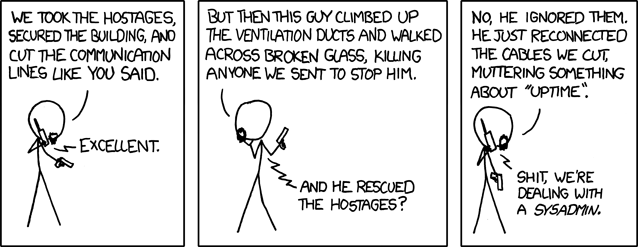
\includegraphics[scale=0.8]{comics/devotion_to_duty}
%\end{center}


%%%%%%%%%%%%%%%%%%%%%%%%%%%%%%%%%%%%%%%%%%%%%%%%%%%%%%%%%%%%%%%%%%%%%%%%%%%
\newpage
\section{Informatiker-Witze}
Warum ist ein Informatiker besser als ein Mathematiker? \\
Dank dem binären Zahlensystem kann er mit den Fingern weiter rechnen!\\


***\\


Ein Physiker, ein Mathematiker und ein  Informatiker bekommen die Aufgabe gestellt, herauszufinden wie viel 1+1 ist.\\
\newline
Als erster versucht sich der Physiker. Er zieht sich in sein Labor zurück und  stöpselt  aufwendige Apparaturen zusammen. Nach doch schon zwei Monaten kommt er zurück und sagt: ''Also genau habe ich’s nicht rausgefunden. Aber das Ergebnis liegt irgendwo zwischen 1,9 und 2,1.'' Naja, das ist ja schon ganz gut. \\
\newline
Als nächster macht sich der Mathematiker an die Arbeit. Er rennt in seinen Raum, wälzt  tonnenweise Fachliteratur und stellt  aufwendige Gleichungssysteme  auf. Nach zwei Wochen verkündet er  schließlich  sein Ergebnis: ''Die gesuchte Zahl liegt im Intervall von 1,99 bis 2,01.'' Ja, schon besser. \\
\newline
Aber jetzt ist der Informatiker an der Reihe. Er geht ins Nebenzimmer und kommt schon nach 2 Minuten zurück. ''Das Ergebnis lautet 2.'' Die beiden anderen sind komplett von den Socken und fragen den Informatiker, wie er denn so schnell auf das Ergebnis gekommen ist. Darauf antwortet der freudestrahlend: “Ist doch ganz einfach! Ich hab in Wikipedia nachgesehen!“\\


***\\


Unterhalten sich ein Mediziner, Ingenieur und ein Informatiker, wer wohl zuerst da war. \\
\newline
Mediziner: Also das war ja wohl ein Mediziner. Denn schon in der Bibel steht, Gott schuf Eva aus der Rippe von Adam. Das ist eindeutig ein chirurgischer Eingriff. \\
\newline
Ingenieur: In der Bibel steht aber, am Anfang war das Chaos. Und man braucht einen Ingenieur, um das aufzuräumen. Daher muss ein Ingenieur der erste gewesen sein. \\
\newline
Da lehnt sich der Informatiker zurück: Und wer, meint Ihr, hat das Chaos erzeugt?\\


***\\


Woran erkennt man einen extrovertierten Informatiker? Er schaut beim Reden auf \textbf{Deine} Schuhe.\\


***\\


Mit Computern hat man Zeit, Dinge zu tun, die man ohne sie nicht tun müsste...\\


***\\


Drei männliche Programmierer im Bad vor den Urinalen: \\
\newline
Der erste ist fertig und geht zum Waschbecken, um sich die Hände zu waschen. Dann trocknet er sich die Hände und ist dabei äußerst gründlich und benutzt ein Papierhandtuch nach dem anderen dabei - streng darauf bedacht, nicht das kleinste Wassertröpfchen auszulassen. Als er fertig ist, sagt er zu den anderen beiden: ''Bei MICROSOFT achten wir darauf, extrem gründlich zu sein.'' \\
\newline
Der zweite ist fertig und geht zum Waschbecken, um sich die Hände zu waschen. Dann trocknet er sich die Hände ab und ist dabei nicht nur gründlich, sondern er benutzt nur ein Blatt Papier, aber davon auch jedes noch so kleine Fitzelchen. Als er fertig ist, sagt er zu den anderen beiden: ''Bei INTEL achten wir nicht nur darauf extrem gründlich zu sein, wir sind auch sehr sparsam.'' \\
\newline
Der dritte ist fertig, geht und ruft: ''Bei APPLE pissen wir uns nicht auf die Hände ...''\\


***\\


Ein Informatiker geht durch den Park (wahrscheinlich hatte der Pizzabringservice Ruhetag und er musste selbst gehen).\\
\newline
Dabei spricht ihn ein Frosch an: ''Ich bin eine verwunschene Prinzessin. Wenn Du mich küsst und heiratest verwandle ich mich zurück und bin für immer Dein!''.\\
\newline
Der Informatiker steckt den Frosch in die Jackentasche und geht weiter. Den Protest aus seiner Jackentasche ignoriert er.\\
\newline
Nach einer Weile nimmt der Protest zu. ''Warum küsst und heiratest Du mich nicht? Ich bin schließlich eine Prinzessin. Wenn auch verwunschen!''\\
\newline
Daraufhin nimmt er den Frosch auf die Hand und sagt: ''Ich bin Informatiker. An einer Freundin habe ich kein Interesse, aber ein sprechender Frosch ist irgendwie cool!''\\


***\\


Zwei Informatiker treffen sich im Park, der eine hat ein neues Fahrrad.\\
\newline
Meint der andere: \\
- Tolles Fahrrad, was hast´n gekostet?\\
- War kostenlos.\\
- Erzähl mal!\\
- Naja, gestern bin ich hier durch den Park gegangen, da kommt ´ne Frau auf ´nem Fahrrad vorbei, hält an, zieht sich die Kleider aus, und meint, ich könnte alles von ihr haben, was ich will.\\
- Hey echt gute Wahl, die Kleider hätten Dir nicht gepasst...\\


***\\


Auf einer Wetterstation musste die tägliche Niederschlagshöhe von Hand in den Computer eingegeben werden.\\
\newline
Irgendwann einmal vertippte sich dabei einer, statt 8,54 cm gab er 8,54 m ein. Die Programmierer hatten aber wohl für diesen Fall vorgesorgt, denn der Computer gab folgende Fehlermeldung aus:\\
''Baue ein Boot! Nimm von jeder Tierart zwei, ein männliches und ein weibliches...''\\


***\\


Sie brauchen einen Computer nicht einzuschalten um festzustellen, ob Windows installiert ist. \\
Sehen Sie einfach nach, ob die Aufschrift auf der Reset-Taste noch lesbar ist.\\


***\\


Die amerikanische Post hat die Verdienste Bill Gates gewürdigt, sein Konterfei ziert eine Briefmarke. Im täglichen Betrieb zeigte sich jedoch, dass diese Briefmarke nicht auf den Briefen hielt. \\
Die eingesetzte Untersuchungskommission kam nach wenigen Monaten zu folgendem Ergebnis:\\
\newline
1. Die Briefmarke ist völlig korrekt.\\
2. Der Kleber ist ebenfalls nicht zu beanstanden.\\
3. Die Kunden spucken nur auf die falsche Seite...\\


***\\


Wissenschaftler wollten wissen, ob Computerstrahlung schädlich ist.\\
Sie sperrten drei Ratten mit einem angeschalteten Computer in einen Käfig, gaben Futter und Wasser zu und ließen das Ganze für eine Woche so stehen.\\
\newline
- Und, sind die Ratten krank geworden?\\
- Nein, aber sie haben drei neue UNIX-Versionen programmiert!\\


***\\


Bill Gates kommt in den Himmel... \\
Da Fragt der Liebe Gott: ''Na mein Sohn, was kann ich für dich tun?'' \\
Darauf antwortet Bill Gates: ''Erstens, ich bin nicht dein Sohn! Und zweitens, runter von meinem Stuhl!''\\


***\\


\textbf{Programmierer und der Prostituierte.}  \\
\newline
Du hast bizarre Arbeitszeiten. \\
- wie die Prostituierten \\
\newline
Du wirst bezahlt, um Deinen Kunden glücklich zu machen. \\
- wie die Prostituierten \\
\newline
Dein Kunde bezahlt viel, aber Dein Chef kassiert das Geld .. \\
- wie bei den Prostituierten \\
\newline
Du hast einen Stundenlohn aber Deine Arbeitszeit endet wenn die Arbeit erledigt ist. \\
- wie bei den Prostituierten \\
\newline
Auch wenn Du gut bist, bist Du nie stolz auf Deine Arbeit .. \\
- wie die Prostituierten \\
\newline
Du wirst bezahlt, um Fantasien Deines Kunden zu befriedigen. \\
- wie die Prostituierten \\
\newline
Es ist schwierig für Dich eine Familie zu haben und zu halten. \\
- wie bei den Prostituierten \\
\newline
Wenn Du gefragt wirst, worin Deine Arbeit besteht, kannst Du es nicht richtig erklären. \\
- wie die Prostituierten \\
\newline
Deine Freunde verlassen Dich und Du bleibst zurück mit Typen wie Dir... \\
- wie die Prostituierten \\
\newline
Der Kunde bezahlt das Hotel und die Arbeitszeit\\
- wie bei den Prostituierten \\
\newline
Dein Boss hat ein wunderschönes Auto. \\
- wie bei den Prostituierten \\
\newline
Wenn Du zu einem Kunden auf ''Mission'' gehst, kommst Du mit einem großen Lächeln an. \\
- wie die Prostituierten \\
\newline
Aber wenn Du deine Arbeit erledigt hast, bist Du schlecht gelaunt .. \\
- wie die Prostituierten \\
\newline
Um Deine Fähigkeiten zu beweisen, musst Du grauenvolle Tests bestehen. \\
- wie die Prostituierten \\
\newline
Der Kunde möchte immer weniger bezahlen und Du muss trotzdem Wunder vollbringen. \\
- wie die Prostituierten \\
\newline
Wenn Du morgens aufstehst, denkst Du: „Ich kanndas nicht ein Leben lang machen“. \\
- wie die Prostituierten\\


***\\


UNIX ist das Betriebssystem der Zukunft. \\
Und das schon seit 30 Jahren.\\


***\\


Ein Apotheker bekam mit den Rechnungen für Arzneimittel auch Bestellformulare.\\
\newline
Als er zweimal keine bekam, legte er einer Bestellung folgende Mitteilung bei:\\
''Ich habe Verständigungsschwierigkeiten mit Ihrem Computer. Wenn Sie keine Bestellformulare mehr versenden, lassen Sie es mich wissen - vorausgesetzt, dass Sie noch Menschen aus Fleisch und Blut beschäftigen.''\\
\newline
Mit der nächsten Lieferung kam die Antwort: ''Beiliegend sechs Bestellformulare. Entschuldigen Sie das Versehen. Wir beschäftigen übrigens noch Menschen, aber das ist eben das Problem. Gezeichnet, IBM 402.''\\


***\\


Bill Gates tippt in seinen Computer: ''Gibt es einen Gott?''\\
Antwort: ''Zu wenig Rechenkapazität.''\\
\newline
Er lässt alle Computer bei Klein und Weich einschließlich des gesamten MSN zusammenschalten und tippt erneut seine Frage ein.\\
Antwort: ''Zu wenig Rechenkapazität.''\\
\newline
Er ruft alle Bekannten bei Cray, Sun, etc. an. Auch diese Computer werden zu einem gigantischen Netzwerk zusammengeschaltet. Erneut tippt er seine Frage ein.\\
Antwort: ''Jetzt ja!...''\\


***\\


Woran erkennt man einen Informatiker? \\
An den roten Augen!\\


***\\


Ein Beweis für Programmierer:\\
- Jedes Programm lässt sich um mindestens eine Anweisung kürzen.\\
- Jedes Programm hat mindestens einen Fehler.\\
\newline
Durch Induktion können wir schließen:\\
- Jedes Programm ist reduzierbar auf eine Anweisung, die nicht funktioniert...\\


***\\


Ein Arzt, ein Anwalt und ein Microsoft-Programmierer streiten sich, ob eine Freundin einer Frau vorzuziehen wäre. \\
\newline
Der Anwalt: ''Klar gibt am wenigsten Probleme bei der Trennung.'' \\
\newline
Daraufhin der Arzt: ''Also ich brauche die Geborgenheit einer Frau.'' \\
\newline
Der Programmier dann: ''Also ich habe beides, denn wenn ich weg bin denkt meine Frau ich bin bei meiner Freundin, und meine Freundin denkt ich bin bei meiner Frau, und ich kann in Ruhe programmieren.''\\


***\\


Anwender1: ''Mein Win Vista ist in 6 Monaten noch nie abgestürzt.''\\
\newline
Anwender2: ''Ein halbes Jahr ohne Strom - das ist hart!''\\


***\\


Streiten sich drei über den besten Computer.\\
\newline
Meint der Erste: ''Echte Männer arbeiten mit einem PC und lassen ihre Kinder mit einem Amiga spielen.''\\
\newline
Darauf der Zweite: ''Echte Männer arbeiten mit einer SUN und geben den PC den Kindern zum spielen.''\\
\newline
Schließlich der Dritte: ''Echte Männer spielen mit ihren Kindern und lassen den MAC für sich arbeiten!''\\


***\\


Eines Tages kam ein Apple-Fanatiker in das Dojo eines Linux Meisters.
Um ihn herum sah er die wild tippenden Schüler und auf allen Bildschirmen waren nur Buchstaben zu sehen.
Da fagte er den Meister:\\
\newline
''Warum benutzt ihr nur die Konsole? Warum benutzt ihr keine Maus?
Ein Bild sagt mehr als tausend Worte. Nutzt doch Icons!
Seht die Funktionalität des iPhone! Es ist einfach und bequem, so dass jeder damit umgehen kann.''\\
\newline
Der Meister sagte nichts und zeigte auf seinen Schüler. Dann zeigte er auf einen Bildschirm, auf seinen Kopf, auf den Fanatiker, auf den Himmel und auf seine Hand.\\
\newline
Der Fanatiker sagte: ''Was willst du mir damit sagen? Ich verstehe nicht.''\\
\newline
Daraufhin sagte der Meister ''Siehst du es nun?'' und der Fanatiker wurde erleuchtet.\\




\begin{flushright} Pavel \end{flushright} 


%\vspace{3cm}
%\begin{minipage}[t]{.4\linewidth}
%\begin{center}
%\includegraphics[scale=0.65]{fotos/fachschaftsraumtuer}
%\end{center}
%\end{minipage}

%%%%%%%%%%%%%%%%%%%%%%%%%%%%%%%%%%%%%%%%%%%%%%%%%%%%%%%%%%%%%%%%%%%%%%%%%%%

\newpage
\section{Ein kleines Nachwort}
%\spaltenanfang
Nun, ihr ahnt es wohl schon. 
Das große Abenteuer OE SS 2014 neigt sich dem Ende zu, und ihr steuert direkt auf einen völlig neuen Abschnitt in eurem Leben zu.


Wir hoffen, dass wir an alle Informationen, die ihr braucht, um ab dem ersten Tag richtig loszulegen zu können, gedacht haben und sie halbwegs verständlich weitergegeben haben. 
Falls dennoch etwas fehlt oder irgendwelche Fragen unbeantwortet geblieben sind, sind wir ja nicht aus der Welt. 
Und wir als Fachschaft sehen mit dem Ende der OE unsere Aufgabe auch keineswegs als beendet an.


Man findet uns manchmal im Lernzentrum, auch in der Student Lounge hat man immer eine gewisse Chance, jemanden zu treffen, der Rat weiß oder jemanden weiß, der Rat weiß, oder jemanden weiß, der einen kennt, der \dots


Lange Rede, kurzer Sinn, wer es mit einer gewissen Ernsthaftigkeit versucht, wird im Allgemeinen keine Probleme haben, jemanden von uns zu finden. 
Wenn wirklich mal überhaupt niemand aufzustöbern sein sollte, so kann man durch das Schicken einer e-Mail an \emailfachschaft\\ oder das Posten in unserem Forum \textbf{\url{http://fsinf-forum.de}} Kontakt aufnehmen. 
Besucht auch unsere Internetpräsenz: \textbf{
\url{http://www.fsinf-frankfurt.de}
}.
Die allersicherste Methode, uns zu finden, ist und bleibt jedoch das Fachschaftstreffen.

\begin{center}
Fachschaftstreffen\\
Am 1. Donnerstag jeden Monats, um 16:00 Uhr\\
in der Student Lounge (Raum hinter dem Lernzentrum)\\
\end{center}


Wir würden uns unheimlich freuen, wenn ihr Lust hättet, uns in unserer Fachschaftsarbeit zu unterstützen. 
Also, einfach mal vorbeischauen! 
Man erfährt meist recht nützliche Dinge über den Fachbereich und hat Gelegenheit, alle Themen, die das Studium betreffen, zur Sprache zu bringen.

%\spaltenende


%%%%%%%%%%%%%%%%%%%%%%%%%%%%%%%%%%%%%%%%%%%%%%%%%%%%%%%%%%%%%%%%%%%%%%%%%%%

\section*{Ende! :-)}

Wir verabschieden uns von euch, wünschen Euch ein erfolgreiches Studium und eine schöne Zeit an der Uni!

%\begin{center}
%	\includegraphics[scale=0.42]{bitmaps/OE2011_tshirt}
%\end{center}
\newpage

%\begin{center}
%\vspace{1cm}
%\includegraphics[scale=0.8]{comics/single/student_verschleiss}
%\end{center}


%%%%%%%%%%%%%%%%%%%%%%%%%%%%%%%%%%%%%%%%%%%%%%%%%%%%%%%%%%%%%%%%%%%%%%%%%%%
%\begin{center}
%\includegraphics[scale=1.0]{comics/single/gluecklich}
%\end{center}
%\vspace{3cm}

\section{Übersicht über den Campus Bockenheim}


%Auf der folgenden Seite findet Ihr abschließend noch einen Lageplan vom Campus Bockenheim. Dieser wird anfangs der Dreh- und Angelpunkt eures Studiums sein.
Hier findet Ihr abschließend noch einen Lageplan vom Campus Bockenheim. Dieser wird anfangs der Dreh- und Angelpunkt eures Studiums sein.


%\newpage
~
\thispagestyle{empty}
%\begin{addmargin}[-12mm]{0mm}
\begin{center}
%\includegraphics[width=0.85\textheight, angle=90]{bitmaps/plan_gross}
%\includegraphics[width=0.9\textwidth]{bitmaps/uni-plan_01_ohne_afe}
%\includegraphics[width=0.9\textwidth]{bitmaps/uni-plan_02_ohne_afe}
\includegraphics[width=0.85\textwidth]{bitmaps/KarteB}
\end{center}
%\end{addmargin}
\newpage



\end{document}
